%%%%%%%%%%%%%%%%%%%%%%%%%%%%%%%%%%%%%%%%%%%%%%%%%%%%%%%%%%%%%%%%%%%%%%%%%%%%
%DIF LATEXDIFF DIFFERENCE FILE
%DIF DEL owp_fim4_expanded_original.tex   Fri Sep 16 22:13:08 2022
%DIF ADD owp_fim4_expanded.tex            Mon Sep 19 13:10:47 2022
% AGUJournalTemplate.tex: this template file is for articles formatted with LaTeX
%
% This file includes commands and instructions
% given in the order necessary to produce a final output that will
% satisfy AGU requirements, including customized APA reference formatting.
%
% You may copy this file and give it your
% article name, and enter your text.
%
%
% Step 1: Set the \documentclass
%
%

%% To submit your paper:
\documentclass[draft]{dependencies/agujournal2019}
\usepackage{url} %this package should fix any errors with URLs in refs.
\usepackage{lineno}
\usepackage[inline]{dependencies/trackchanges} %for better track changes. finalnew option will compile document with changes incorporated.
\usepackage{soul}
%DIF 22a22
\usepackage{rotating} %DIF > 
%DIF -------

%% added
\usepackage{multirow}
\usepackage{amsmath}
%DIF 26a27
\usepackage{float} %DIF > 
%DIF -------

\linenumbers

%%%%%%%
% As of 2018 we recommend use of the TrackChanges package to mark revisions.
% Add track changes editors
\addeditor{Fernando Aristizabal}

% The trackchanges package adds five new LaTeX commands:
%
%  \note[editor]{The note}
%  \annote[editor]{Text to annotate}{The note}
%  \add[editor]{Text to add}
%  \remove[editor]{Text to remove}
%  \change[editor]{Text to remove}{Text to add}
%
% complete documentation is here: http://trackchanges.sourceforge.net/
%%%%%%%

\drafttrue

%% Enter journal name below.
%% Choose from this list of Journals:
%
% JGR: Atmospheres
% JGR: Biogeosciences
% JGR: Earth Surface
% JGR: Oceans
% JGR: Planets
% JGR: Solid Earth
% JGR: Space Physics
% Global Biogeochemical Cycles
% Geophysical Research Letters
% Paleoceanography and Paleoclimatology
% Radio Science
% Reviews of Geophysics
% Tectonics
% Space Weather
% Water Resources Research
% Geochemistry, Geophysics, Geosystems
% Journal of Advances in Modeling Earth Systems (JAMES)
% Earth's Future
% Earth and Space Science
% Geohealth
%
% ie, \journalname{Water Resources Research}

\journalname{Water Resources Research}


% starts document
%DIF PREAMBLE EXTENSION ADDED BY LATEXDIFF
%DIF UNDERLINE PREAMBLE %DIF PREAMBLE
\RequirePackage[normalem]{ulem} %DIF PREAMBLE
\RequirePackage{color}\definecolor{RED}{rgb}{1,0,0}\definecolor{BLUE}{rgb}{0,0,1} %DIF PREAMBLE
\providecommand{\DIFadd}[1]{{\protect\color{blue}\uwave{#1}}} %DIF PREAMBLE
\providecommand{\DIFdel}[1]{{\protect\color{red}\sout{#1}}}                      %DIF PREAMBLE
%DIF SAFE PREAMBLE %DIF PREAMBLE
\providecommand{\DIFaddbegin}{} %DIF PREAMBLE
\providecommand{\DIFaddend}{} %DIF PREAMBLE
\providecommand{\DIFdelbegin}{} %DIF PREAMBLE
\providecommand{\DIFdelend}{} %DIF PREAMBLE
\providecommand{\DIFmodbegin}{} %DIF PREAMBLE
\providecommand{\DIFmodend}{} %DIF PREAMBLE
%DIF FLOATSAFE PREAMBLE %DIF PREAMBLE
\providecommand{\DIFaddFL}[1]{\DIFadd{#1}} %DIF PREAMBLE
\providecommand{\DIFdelFL}[1]{\DIFdel{#1}} %DIF PREAMBLE
\providecommand{\DIFaddbeginFL}{} %DIF PREAMBLE
\providecommand{\DIFaddendFL}{} %DIF PREAMBLE
\providecommand{\DIFdelbeginFL}{} %DIF PREAMBLE
\providecommand{\DIFdelendFL}{} %DIF PREAMBLE
%DIF COLORLISTINGS PREAMBLE %DIF PREAMBLE
\RequirePackage{listings} %DIF PREAMBLE
\RequirePackage{color} %DIF PREAMBLE
\lstdefinelanguage{DIFcode}{ %DIF PREAMBLE
%DIF DIFCODE_UNDERLINE %DIF PREAMBLE
  moredelim=[il][\color{red}\sout]{\%DIF\ <\ }, %DIF PREAMBLE
  moredelim=[il][\color{blue}\uwave]{\%DIF\ >\ } %DIF PREAMBLE
} %DIF PREAMBLE
\lstdefinestyle{DIFverbatimstyle}{ %DIF PREAMBLE
	language=DIFcode, %DIF PREAMBLE
	basicstyle=\ttfamily, %DIF PREAMBLE
	columns=fullflexible, %DIF PREAMBLE
	keepspaces=true %DIF PREAMBLE
} %DIF PREAMBLE
\lstnewenvironment{DIFverbatim}{\lstset{style=DIFverbatimstyle}}{} %DIF PREAMBLE
\lstnewenvironment{DIFverbatim*}{\lstset{style=DIFverbatimstyle,showspaces=true}}{} %DIF PREAMBLE
%DIF END PREAMBLE EXTENSION ADDED BY LATEXDIFF

\begin{document}


%% Title and Authors
%% ------------------------------------------------------------------------ %%
%  Title
%
% (A title should be specific, informative, and brief. Use
% abbreviations only if they are defined in the abstract. Titles that
% start with general keywords then specific terms are optimized in
% searches)
%
%% ------------------------------------------------------------------------ %%

% Example: \title{This is a test title}
%
%DIF > \title{Reducing Horton-Strahler Stream Order Can Enhance Flood Inundation Mapping Skill with Applications for the U.S. National Water Model}
\title{\DIFdelbegin \DIFdel{Reducing Horton-Strahler Stream Order Can Enhance }\DIFdelend \DIFaddbegin \DIFadd{Extending Height Above Nearest Drainage to Model Multiple Fluvial Sources in }\DIFaddend Flood Inundation Mapping \DIFdelbegin \DIFdel{Skill with }\DIFdelend Applications for the U.S. National Water Model}
%
%% ------------------------------------------------------------------------ %%
%
%  AUTHORS AND AFFILIATIONS
%
%% ------------------------------------------------------------------------ %%

% Authors are individuals who have significantly contributed to the
% research and preparation of the article. Group authors are allowed, if
% each author in the group is separately identified in an appendix.)

% List authors by first name or initial followed by last name and
% separated by commas. Use \affil{} to number affiliations, and
% \thanks{} for author notes.
% Additional author notes should be indicated with \thanks{} (for
% example, for current addresses).

% Example: \authors{A. B. Author\affil{1}\thanks{Current address, Antartica}, B. C. Author\affil{2,3}, and D. E.
% Author\affil{3,4}\thanks{Also funded by Monsanto.}}
%
%
\authors{Fernando Aristizabal\affil{1,2,3}, Fernando Salas\affil{3}, Gregory Petrochenkov\affil{4}, Trevor Grout\affil{1,3}, Brian Avant\affil{1,3}, Bradford Bates\affil{1,3}, Ryan Spies\affil{1,3}, Nick Chadwick\affil{3}, Zachary Wills\affil{3,5}, Jasmeet Judge\affil{2}}
%
%
\affiliation{1}{Lynker, Leesburg, VA, USA}
\affiliation{2}{Center for Remote Sensing, Agricultural and Biological Engineering Department, University of Florida, Gainesville, FL, USA}
\affiliation{3}{National Water Center, Office of Water Prediction, National Weather Service, National Oceanic and Atmospheric Administration, Tuscaloosa, AL, USA}
\DIFdelbegin %DIFDELCMD < \affiliation{4}{New York Water Science Center, Hydrologic Applied Innovations Lab, United States Geological Survey, Troy, NY, USA}
%DIFDELCMD < %%%
\DIFdelend \DIFaddbegin \affiliation{4}{Hydrologic Applied Innovations Lab, New York Water Science Center, United States Geological Survey, Troy, NY, USA}
\DIFaddend \affiliation{5}{Cooperative Institute for Satellite Earth System Studies, University of Maryland, College Park, MD, USA}
%
%(repeat as many times as is necessary)
%
%% Corresponding Author:
% Corresponding author mailing address and e-mail address:

% (include name and email addresses of the corresponding author.  More
% than one corresponding author is allowed in this LaTeX file and for
% publication; but only one corresponding author is allowed in our
% editorial system.)
%
% Example: \correspondingauthor{First and Last Name}{email@address.edu}
%
\correspondingauthor{Fernando Aristizabal}{fernando.aristizabal@noaa.gov}


%% Keypoints
%% Keypoints, final entry on title page.

%  List up to three key points (at least one is required)
%  Key Points summarize the main points and conclusions of the article
%  Each must be 140 characters or fewer with no special characters or punctuation and must be complete sentences

% Example:
% \begin{keypoints}
% \item	List up to three key points (at least one is required)
% \item	Key Points summarize the main points and conclusions of the article
% \item	Each must be 140 characters or fewer with no special characters or punctuation and must be complete sentences
% \end{keypoints}
%
\begin{keypoints}
\item Flood \DIFdelbegin \DIFdel{inundation }\DIFdelend maps derived from Height Above Nearest Drainage (HAND) are subject to \DIFdelbegin \DIFdel{limitations at river junctions}\DIFdelend \DIFaddbegin \DIFadd{nearest drainage line limitations that affect inundation skill}\DIFaddend .
\item A means of resolving this limitation is provided by reducing HAND processing units to level paths \DIFdelbegin \DIFdel{of }\DIFdelend \DIFaddbegin \DIFadd{with effective }\DIFaddend unit stream order.
\item \DIFdelbegin \DIFdel{Changing the scale of the }\DIFdelend \DIFaddbegin \DIFadd{Discretizing the }\DIFaddend stream network for HAND \DIFdelbegin \DIFdel{processing }\DIFdelend \DIFaddbegin \DIFadd{computation }\DIFaddend affects the stage-discharge relationship and leads to higher skill inundation.
\end{keypoints}
%


%% Abstract
% ------------------------------------------------------------------------ %%
%
%  ABSTRACT and PLAIN LANGUAGE SUMMARY
%
% A good Abstract will begin with a short description of the problem
% being addressed, briefly describe the new data or analyses, then
% briefly states the main conclusion(s) and how they are supported and
% uncertainties.

% The Plain Language Summary should be written for a broad audience,
% including journalists and the science-interested public, that will not have 
% a background in your field.
%
% A Plain Language Summary is required in GRL, JGR: Planets, JGR: Biogeosciences,
% JGR: Oceans, G-Cubed, Reviews of Geophysics, and JAMES.
% see http://sharingscience.agu.org/creating-plain-language-summary/)
%
%% ------------------------------------------------------------------------ %%

%% \begin{abstract} starts the second page

\begin{abstract}
\DIFdelbegin \DIFdel{The National Water Model (NWM) currently requires the post-processing of forecast discharges to produce forecast flood inundation maps (FIM) for protecting life and property. 
}\DIFdelend Height Above Nearest Drainage (HAND), a drainage normalizing terrain index, is \DIFdelbegin \DIFdel{worthy of producing high-resolution FIMsat large spatial scales and frequent time steps }\DIFdelend \DIFaddbegin \DIFadd{a means able of producing high resolution flood inundation maps (FIMs) from the National Water Model (NWM) at large scales and high resolutions }\DIFaddend using reach-averaged synthetic rating curves. 
\DIFdelbegin \DIFdel{However, HAND based FIMs suffer from a known limitation caused by independent catchments that lack }\DIFdelend \DIFaddbegin \DIFadd{We highlight here that HAND is limited to producing inundation only when sourced from its nearest drainage line, thus lacks }\DIFaddend the ability to \DIFdelbegin \DIFdel{cross catchment boundaries and ridgelines.
To counter this constraint, a }\DIFdelend \DIFaddbegin \DIFadd{source inundation from multiple fluvial sources.
A }\DIFaddend version of HAND\DIFaddbegin \DIFadd{, }\DIFaddend known as Generalized Mainstems (GMS)\DIFaddbegin \DIFadd{, }\DIFaddend is proposed that \DIFdelbegin \DIFdel{reduces the Horton-Strahler stream order of the stream network .
GMS contains all segments within the NWM stream network but instead of deriving HAND by accounting for all river segments at once, it is derived independently at the level path }\DIFdelend \DIFaddbegin \DIFadd{discretizes a target stream network into segments of unit Horton-Strahler stream order known as level paths }\DIFaddend (LP)\DIFdelbegin \DIFdel{scale.
LPs are unique identifiers propagated upstream from a sub-basin’s outlet along the direction of maximum flow distance and repeated recursively until all segments are assigned LP identifiers.
These FIMs }\DIFdelend \DIFaddbegin \DIFadd{.
The FIMs associated with each independent LP }\DIFaddend are then mosaiced together, effectively turning the stream network into discrete groups of \DIFdelbegin \DIFdel{homogenous }\DIFdelend \DIFaddbegin \DIFadd{homogeneous }\DIFaddend unit stream order by removing the influence of neighboring tributaries.
Improvement in mapping skill is observed \DIFdelbegin \DIFdel{when compared to HEC-RAS 1D models }\DIFdelend by significantly reducing false negatives at river junctions \DIFaddbegin \DIFadd{when the inundation extents are compared to FIMs from that of benchmarks}\DIFaddend .
A more marginal reduction in the false alarm rate is also observed due to a \DIFdelbegin \DIFdel{bias }\DIFdelend \DIFaddbegin \DIFadd{shift }\DIFaddend introduced in the stage-discharge relationship by increasing the size of the catchments.
\DIFaddbegin \DIFadd{We observe that the improvement of this method applied at 4-5\% of the entire stream network to 100\% of the network is about the same magnitude improvement as going from no drainage order reduction to 4-5\% of the network.
This novel contribution is framed in a new open-source implementation that utilizes the latest combination of hydro-conditioning techniques to enforce drainage and counter limitations in the input data.
}\DIFaddend \end{abstract}
%
\section*{Plain Language Summary}
Flooding is one of the most impactful natural disasters on life and property.
The United States National Water Model (NWM) provides flood forecasts for the entire country so that adequate warnings can be raised to the public to enable safe evacuations and protective measures.
In order to convert \DIFdelbegin \DIFdel{forecasted }\DIFdelend flow rates from the NWM to flood inundation maps (FIM), a model\DIFaddbegin \DIFadd{, known as Height Above Nearest Drainage (HAND), }\DIFaddend is used that converts elevation data from height above mean sea-level to height above the nearest river bottom.
This model \DIFdelbegin \DIFdel{known as Height Above Nearest Drainage (HAND) }\DIFdelend suffers from issues in mapping performance \DIFdelbegin \DIFdel{where rivers converge}\DIFdelend \DIFaddbegin \DIFadd{because inundation sourced from rivers is only considered from the nearest river line}\DIFaddend .
We developed a technique that mitigates these errors by removing consideration for neighboring tributaries in the relative elevation computation process.
\DIFaddbegin \DIFadd{This is done by splitting the stream network into continuous river segments known as level paths (LPs).
These LPs have no tributaries, thus are known to be stream lines with a unit stream order indicating no branching.
HAND is computed independently for each LP and the resulting FIMs are mosaiced together to form one seamless map.
}\DIFaddend We compared these HAND derived FIMs to maps from \DIFdelbegin \DIFdel{more realistic }\DIFdelend \DIFaddbegin \DIFadd{physically-based }\DIFaddend models and found improvement in mapping performance.
%


%%% Suggested section heads:
% \section{Introduction}
%
% The main text should start with an introduction. Except for short
% manuscripts (such as comments and replies), the text should be divided
% into sections, each with its own heading.

% Headings should be sentence fragments and do not begin with a
% lowercase letter or number. Examples of good headings are:

% \section{Materials and Methods}
% Here is text on Materials and Methods.
%
% \subsection{A descriptive heading about methods}
% More about Methods.
%
% \section{Data} (Or section title might be a descriptive heading about data)
%
% \section{Results} (Or section title might be a descriptive heading about the
% results)
%
% \section{Conclusions}

% Introduction
%%%%%%%%%%%%%%%%%%%%%%%%%%%%%%%%%%%%%%%%%%%%%%%%%%%%%%%%
\section{Introduction}
%%%%%%%%%%%%%%%%%%%%%%%%%%%%%%%%%%%%%%%%%%%%%%%%%%%%%%%%
%
Flooding is one of the most significant natural disasters in the United States (US) affecting both the loss of life and property. 
In 2017 and 2019, river and flash flooding combined represented the leading cause of death and the second leading cause in 2018 among all natural disasters in the US \cite{national_weather_service_2020,national_weather_service_2019,national_weather_service_2018}. 
More than an average of 104 deaths per year are attributed to flood events from the 10 year period ending in 2019 \cite{us_department_of_commerce_2020}. 
With respect to property damages, river and flash flooding have contributed to 60.7, 1.6, and 3.7 billion non-inflation adjusted US dollars in the annual periods of 2017 to 2019, respectively \cite{national_weather_service_2020,national_weather_service_2019,national_weather_service_2018}\DIFaddbegin \DIFadd{, }\DIFaddend with the large spike in 2017 attributed to the Hurricane Harvey event along the Gulf \DIFdelbegin \DIFdel{coast}\DIFdelend \DIFaddbegin \DIFadd{Coast}\DIFaddend . 
Trends related to flood damages and fatalities have been steadily increasing over recent decades \DIFdelbegin \DIFdel{. }\DIFdelend \cite{mallakpour2015changing,downton2005reanalysis,kunkel1999temporal,pielke2000precipitation,corringham2019effect}. 
Some are expecting that the hydrologic cycle will intensify \DIFaddbegin \DIFadd{due to climate change }\DIFaddend which will lead to more extreme precipitation in some areas along with a greater risk of flooding \cite{tabari2020climate,milly2002increasing,wing2018estimates}. 
Increasing trends in frequency and risk are not uniform across spatial regions with work by \citeA{slater2016recent} indicating that trends are increasing across the US Midwest \DIFdelbegin \DIFdel{/Great Lakes region }\DIFdelend \DIFaddbegin \DIFadd{and Great Lakes regions }\DIFaddend while decreasing in \DIFaddbegin \DIFadd{the }\DIFaddend coastal Southeast, Southwest\DIFaddbegin \DIFadd{, }\DIFaddend and California.
%
%%%%%%%%%%%%%%%%%%%%%%%%%%%%%%%%%%%%%%%%%%%%%%%%%%%%%%%%
\subsection{Operational Forecasting}
%%%%%%%%%%%%%%%%%%%%%%%%%%%%%%%%%%%%%%%%%%%%%%%%%%%%%%%%
%
Operational flood forecasting systems are primary tools in developing accurate forecasts for public awareness prior to life \DIFdelbegin \DIFdel{or }\DIFdelend \DIFaddbegin \DIFadd{threatening and }\DIFaddend property damaging events\DIFdelbegin \DIFdel{occur}\DIFdelend . 
One of these operational systems is the Advanced Hydrologic Prediction System (AHPS) maintained by the National Oceanic Atmospheric Administration (NOAA) National Weather Service (NWS) with thousands of forecasting points across the US at typically short forecast horizons of 24 or 72 hours \cite{mcenery2005noaa}.
AHPS provides forecasting services in the form of ensemble \DIFdelbegin \DIFdel{stream flows }\DIFdelend \DIFaddbegin \DIFadd{streamflows }\DIFaddend at more than 3,600 locations and flood inundation maps (FIM) at more than 150 of those points shown in Figure \ref{fig:forecast_points}.
Additionally, two forecasting networks\DIFaddbegin \DIFadd{, Full Resolution (FR) and Mainstems (MS) stream networks, }\DIFaddend relevant to the National Water Model (NWM) \DIFdelbegin \DIFdel{which will be introduced in Section \ref{ssec:national_water_model}}\DIFdelend \DIFaddbegin \DIFadd{(see Section \ref{ssec:national_water_model}) }\DIFaddend are rendered in Figure \ref{fig:forecast_points}.
\DIFdelbegin \DIFdel{AHPS implements a series of advances including model calibration techniques \mbox{%DIFAUXCMD
\cite{zhang2003hydrologic,hogue2003multi,duan2003global,gupta2003advances,parada2003multi}}\hskip0pt%DIFAUXCMD
, distributed modeling approaches \mbox{%DIFAUXCMD
\cite{reed2004overall,koren2004hydrology,duan2002results}}\hskip0pt%DIFAUXCMD
, ensemble forecasting \mbox{%DIFAUXCMD
\cite{day1985extended,seo2000simulation,mullusky2002simplified,herr2002simplified}}\hskip0pt%DIFAUXCMD
, enhanced data analysis procedures \mbox{%DIFAUXCMD
\cite{mcenery2005noaa}}\hskip0pt%DIFAUXCMD
, flood-forecasting inundation maps \mbox{%DIFAUXCMD
\cite{cajina2002fldview}}\hskip0pt%DIFAUXCMD
, hydraulic routing models \mbox{%DIFAUXCMD
\cite{fread1973technique,cajina2002fldview}}\hskip0pt%DIFAUXCMD
, and multi-sensor precipitation techniques \mbox{%DIFAUXCMD
\cite{breidenbach1999accounting,kondragunta2001outlier,seo2002real,bonnin1996noaa}}\hskip0pt%DIFAUXCMD
}\DIFdelend \DIFaddbegin \DIFadd{The FR network refers to the entire NWM forecasting domain while MS refers to the subset of the FR network that is at or downstream of AHPS forecasting points (see Section \ref{ssec:national_water_model})}\DIFaddend .
On an approximate basis, there is only one forecast point every 1,450 km of river \DIFaddbegin \DIFadd{(FR) }\DIFaddend and one forecast point with FIM every 29,000 km \DIFaddbegin \DIFadd{of river (FR)}\DIFaddend .
Despite the AHPS advances in operational flood forecasting, it lacks sufficient \DIFdelbegin \DIFdel{spatial coverage}\DIFdelend \DIFaddbegin \DIFadd{domain coverage, spatial resolution, }\DIFaddend and long-range forecast horizons to address the increasingly complex water challenges facing the US.
%
\DIFdelbegin %DIFDELCMD < \begin{figure}[h!]
%DIFDELCMD < %%%
\DIFdelendFL \DIFaddbeginFL \begin{figure}[H]
\DIFaddendFL \centering
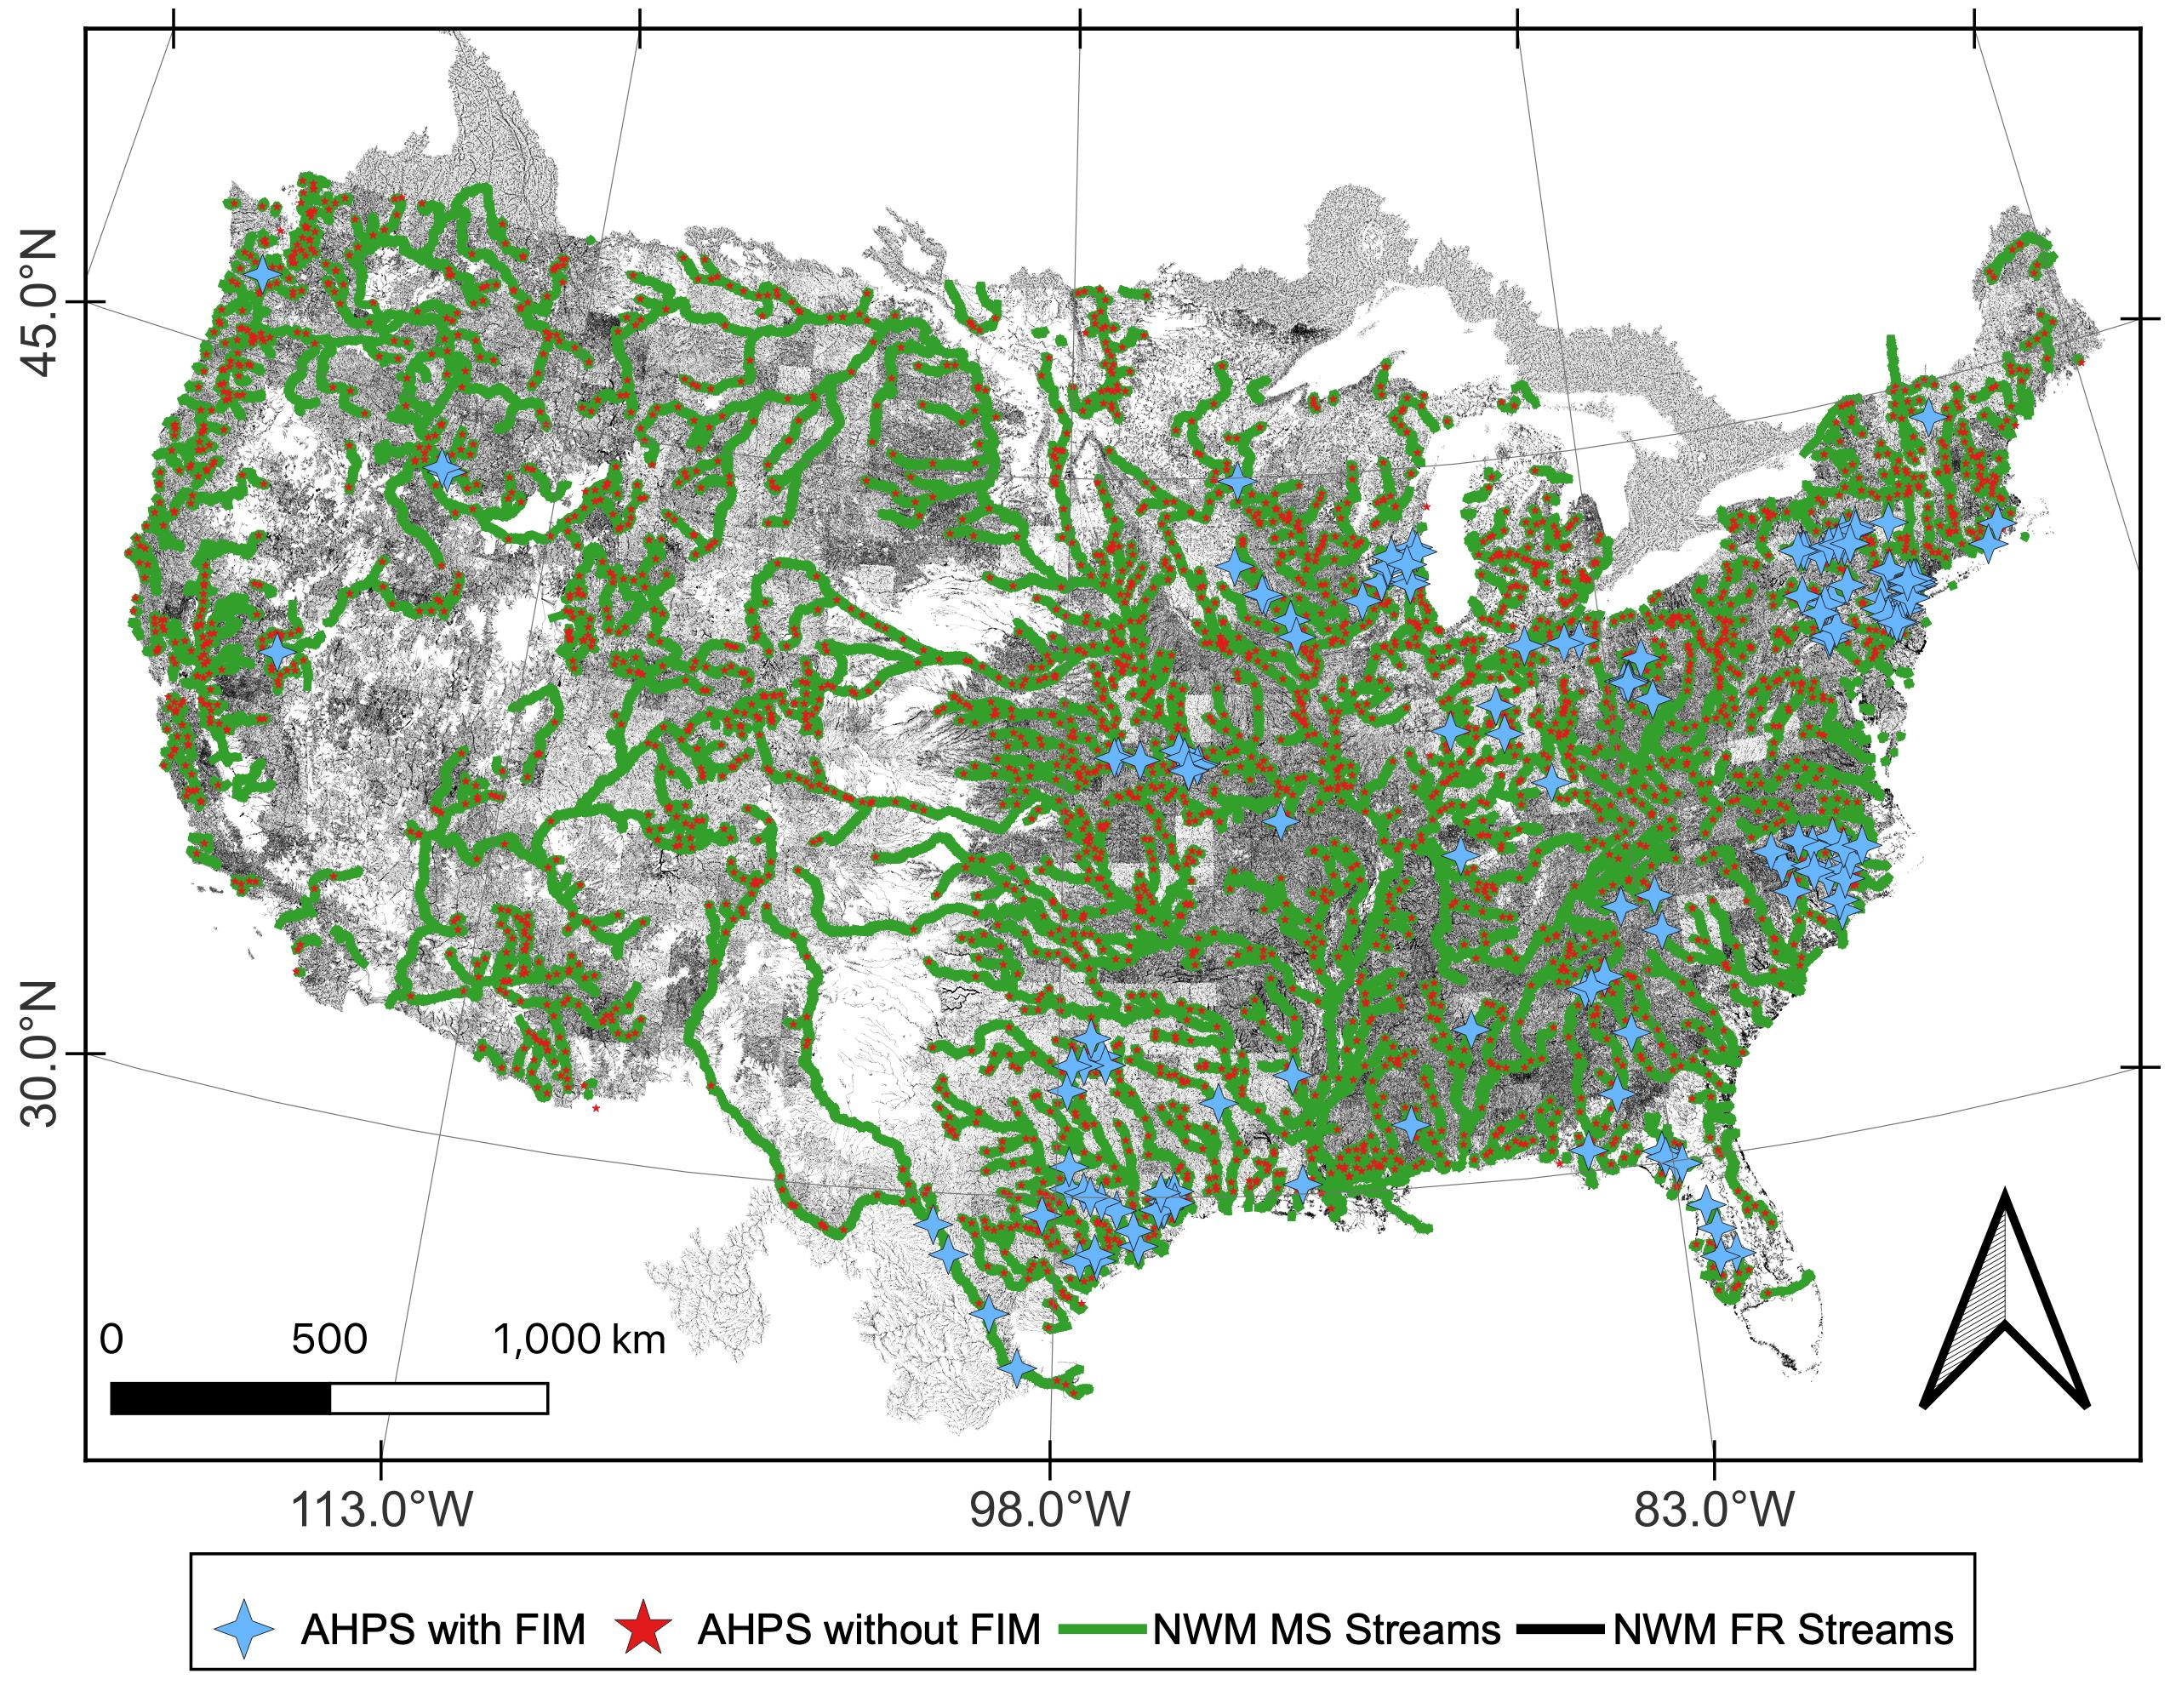
\includegraphics[scale=1.0]{figures/forecast_points.jpg}
\caption{Forecast points with and without \DIFaddbeginFL \DIFaddFL{Flood Inundation Maps (}\DIFaddendFL FIM\DIFaddbeginFL \DIFaddFL{) }\DIFaddendFL in United States' Advanced Hydrologic Prediction System \DIFaddbeginFL \DIFaddFL{(AHPS)}\DIFaddendFL .
\DIFaddbeginFL \DIFaddFL{Note that only a small fraction of the AHPS forecast points have existing FIM.
}\DIFaddendFL Also \DIFdelbeginFL \DIFdelFL{show }\DIFdelendFL \DIFaddbeginFL \DIFaddFL{shown }\DIFaddendFL are the National Water Model \DIFaddbeginFL \DIFaddFL{(NWM) }\DIFaddendFL stream networks at the \DIFdelbeginFL \DIFdelFL{full resolution }\DIFdelendFL \DIFaddbeginFL \DIFaddFL{Full Resolution }\DIFaddendFL (FR) and Mainstems (MS) resolution.
\DIFaddbeginFL \DIFaddFL{The FR network constitutes the entire NWM stream network while the MS resolution network is the FR network at or downstream of the AHPS forecast points shown.
}\DIFaddendFL }
\label{fig:forecast_points}
\end{figure}
%
%%%%%%%%%%%%%%%%%%%%%%%%%%%%%%%%%%%%%%%%%%%%%%%%%%%%%%%%
\subsection{National Water Model}
\label{ssec:national_water_model}
%%%%%%%%%%%%%%%%%%%%%%%%%%%%%%%%%%%%%%%%%%%%%%%%%%%%%%%%
%
Additional work is required to \DIFdelbegin \DIFdel{fill-in }\DIFdelend \DIFaddbegin \DIFadd{address }\DIFaddend the gaps that the AHPS leaves in terms of spatial \DIFdelbegin \DIFdel{and temporal coverage}\DIFdelend \DIFaddbegin \DIFadd{resolution, spatial coverage, and temporal forecast horizons}\DIFaddend .
In response to growing stakeholder demand for enhanced and integrated water resource forecasts, the Office of Water Prediction (OWP) at the National Water Center (NWC) along with its partners \DIFdelbegin \DIFdel{has }\DIFdelend \DIFaddbegin \DIFadd{at the National Center for Atmospheric Research (NCAR) have }\DIFaddend developed and implemented operationally the \DIFdelbegin \DIFdel{National Water Model (NWM ) }\DIFdelend \DIFaddbegin \DIFadd{NWM }\DIFaddend which is a \DIFdelbegin \DIFdel{version }\DIFdelend \DIFaddbegin \DIFadd{configuration }\DIFaddend of the Weather Research and \DIFdelbegin \DIFdel{Forecast }\DIFdelend \DIFaddbegin \DIFadd{Forecasting }\DIFaddend Hydrologic Model (WRF-Hydro) \DIFdelbegin \DIFdel{\mbox{%DIFAUXCMD
\cite{gochis2018wrf,cosgrove2019evolution}}\hskip0pt%DIFAUXCMD
}\DIFdelend \DIFaddbegin \DIFadd{\mbox{%DIFAUXCMD
\cite{salas2018towards,gochis2021wrf,cosgrove2019evolution}}\hskip0pt%DIFAUXCMD
}\DIFaddend . 
The NWM forecasts river discharges at more than 2.7 million forecast points at a variety of time horizons including \DIFdelbegin \DIFdel{some medium (}\DIFdelend \DIFaddbegin \DIFadd{lookback-range (3-28 hrs), short-range (18 hr), medium-range (}\DIFaddend 10 day) and \DIFdelbegin \DIFdel{long }\DIFdelend \DIFaddbegin \DIFadd{long-range }\DIFaddend (30 day) \DIFdelbegin \DIFdel{range }\DIFdelend forecast horizons.
The NWM enhances the spatial and temporal domain of the current AHPS capabilities operated at the 13 River Forecast Centers (RFC) in areas known as `hydro-blind'.
As a complement to the operational NWM, \DIFdelbegin \DIFdel{OWP has also developed a configuration of the NWM that extends RFC forecasts downstream by assimilating and routing forecast streamflows }\DIFdelend \DIFaddbegin \DIFadd{RFC forecasts from AHPS forecast points are assimilated in the NWM and routed downstream }\DIFaddend to the next downstream AHPS forecast point \DIFdelbegin \DIFdel{.
This configuration of }\DIFdelend \DIFaddbegin \DIFadd{where the process iterates again.
This assimilation into }\DIFaddend the NWM is used to enhance forecasting skill by leveraging best available regional-scale \DIFdelbegin \DIFdel{data}\DIFdelend \DIFaddbegin \DIFadd{forecasts}\DIFaddend .
The river network upon which this special \DIFdelbegin \DIFdel{configuration operates }\DIFdelend \DIFaddbegin \DIFadd{assimilation technique operates on }\DIFaddend is herein referred to as the \DIFdelbegin \DIFdel{Main-Stem }\DIFdelend \DIFaddbegin \DIFadd{Mainstem }\DIFaddend (MS) \DIFdelbegin \DIFdel{modeling }\DIFdelend stream network.
Figure \DIFdelbegin \DIFdel{\ref{ssec:national_water_model} shows the Full-Resolution (FR ) modeling }\DIFdelend \DIFaddbegin \DIFadd{\ref{fig:forecast_points} shows the NWM V2.1 FR }\DIFaddend stream network as well as the \DIFaddbegin \DIFadd{NWM V2.1 }\DIFaddend MS network.
The MS network contains roughly 120 thousand forecasting points or roughly 4.4\% of the reaches of the FR stream network.

The National Hydrography Dataset Plus (NHDPlus) V2.1 is the basis for the \DIFdelbegin \DIFdel{hydrofabric }\DIFdelend \DIFaddbegin \DIFadd{``hydrofabric'' }\DIFaddend in the NWM due to its comprehensive use with the hydrologic communities' stakeholders \DIFdelbegin \DIFdel{\mbox{%DIFAUXCMD
\cite{mckay2012nhdplus}}\hskip0pt%DIFAUXCMD
}\DIFdelend \DIFaddbegin \DIFadd{\mbox{%DIFAUXCMD
\cite{mckay2012nhdplus,nhdplus2022vectors}}\hskip0pt%DIFAUXCMD
}\DIFaddend . 
The term \DIFdelbegin \DIFdel{hydrofabric }\DIFdelend \DIFaddbegin \DIFadd{``hydrofabric'' }\DIFaddend is used within the NWM jargon to describe the subset of hydrography composed of the geospatial datasets required for hydrologic modeling including but not limited to stream networks, catchments, channel properties, and elevation data. 
The \DIFdelbegin \DIFdel{Muskingam-Cunge routing method is used within the NWM }\DIFdelend \DIFaddbegin \DIFadd{NWM provides stream forecasts at these hydrofabric segments using the Muskingum-Cunge method }\DIFaddend to reduce computational requirements of a continental scale model \DIFdelbegin \DIFdel{\mbox{%DIFAUXCMD
\cite{bedient2008hydrology,ponce1994variable,gochis2018wrf}}\hskip0pt%DIFAUXCMD
.
Muskingam-Cunge routing scheme has been demonstrated by \mbox{%DIFAUXCMD
\citeA{cunge1969subject} }\hskip0pt%DIFAUXCMD
to be equivalent to the convective-diffusive wave method without consideration to wave dampening.
As a result of high computational costs and large spatial domains, the need for high-resolution }\DIFdelend \DIFaddbegin \DIFadd{but fails to consider backwater dynamics \mbox{%DIFAUXCMD
\cite{bedient2008hydrology,ponce1994variable,gochis2021wrf}}\hskip0pt%DIFAUXCMD
.
The need for high resolution }\DIFaddend FIM at 10 m or better requires additional post-processing from the principal output of the NWM which is forecast river discharges at the reach scale.
The \DIFaddbegin \DIFadd{use of a 2-dimensional (2D) hydrodynamic model across a continental-scale and high spatial resolutions is very cost prohibitive especially in an operational setting.
The }\DIFaddend Height Above Nearest Drainage (HAND) terrain model is one such technique that can be used, along with synthetic rating curves (SRC), to convert \DIFaddbegin \DIFadd{1-dimensional (1D) }\DIFaddend riverine discharges to stages\DIFdelbegin \DIFdel{then }\DIFdelend \DIFaddbegin \DIFadd{, and }\DIFaddend finally to inundation extents \DIFaddbegin \DIFadd{and depths}\DIFaddend .
%
%%%%%%%%%%%%%%%%%%%%%%%%%%%%%%%%%%%%%%%%%%%%%%%%%%%%%%%%
\subsection{Height Above Nearest Drainage}
%%%%%%%%%%%%%%%%%%%%%%%%%%%%%%%%%%%%%%%%%%%%%%%%%%%%%%%%
%
HAND normalizes topography along the nearest drainage path and \DIFdelbegin \DIFdel{its }\DIFdelend \DIFaddbegin \DIFadd{it has }\DIFaddend been demonstrated to be a good proxy and indicator of a series of important environmental conditions including soil environments, landscape classes, soil gravitational potentials, geomorphologies, soil moisture, and groundwater dynamics \cite{renno2008hand,nobre2011height}. 
\citeA{nobre2016hand} showed evidence for utilizing the drainage normalizing HAND dataset as a proxy for flood potential to make static flood inundation maps from known stages.
\DIFdelbegin \DIFdel{A core assumption made for HAND based FIM is enforcing drainage across the entire area of interest which requires significant digital elevation maps (DEM) manipulations to make a reality.
}\DIFdelend The terrain index \DIFdelbegin \DIFdel{has even gone on to provide }\DIFdelend \DIFaddbegin \DIFadd{also provides }\DIFaddend additional utility in the observation of riverine flood inundation mapping from remote sensing especially in areas of high electromagnetic interference such as vegetated and anthropogenic areas \DIFdelbegin \DIFdel{\mbox{%DIFAUXCMD
\cite{aristizabal2020high,shastry2019using,huang2017comparison,twele2016sentinel}}\hskip0pt%DIFAUXCMD
}\DIFdelend \DIFaddbegin \DIFadd{\mbox{%DIFAUXCMD
\cite{aristizabal2020high,shastry2019using,huang2017comparison,twele2016sentinel,aristizabal2021mapping}}\hskip0pt%DIFAUXCMD
}\DIFaddend .
\citeA{zheng2018river} developed a methodology for determining stage-discharge relationships known as \DIFdelbegin \DIFdel{synthetic rating curves (SRC) }\DIFdelend \DIFaddbegin \DIFadd{SRCs }\DIFaddend by sampling reach-averaged parameters from HAND datasets and inputting into the Manning's equation \cite{gauckler1867etudes,manning1890flow}.
This collection of methods, coupling HAND with SRCs, have been experimented with and compared to other sources of FIM including engineering scale models, in-situ observation, and remote sensing based observation with solid results in large spatial scale applications \cite{godbout2019error,johnson2019integrated,garousi2019terrain,nobre2016hand,afshari2018comparison,zheng2018geoflood,teng2015rapid,teng2017flood,zhang2018comparative}.
%
%%%%%%%%%%%%%%%%%%%%%%%%%%%%%%%%%%%%%%%%%%%%%%%%%%%%%%%%
\DIFaddbegin \subsection{\DIFadd{HAND's Assumptions and Limitations}}
\label{sssec:hand_assumptions_limitations}
%DIF > %%%%%%%%%%%%%%%%%%%%%%%%%%%%%%%%%%%%%%%%%%%%%%%%%%%%%%%
%DIF > 
\DIFadd{HAND operates on many underlying assumptions since it can only be used as an inundation proxy or no physics model and thus, not a true hydrodynamic inundation model \mbox{%DIFAUXCMD
\cite{nobre2016hand,liu2016cybergis,liu2020height}}\hskip0pt%DIFAUXCMD
.
HAND, to our knowledge, has only been applied to natural, inland, and riverine inundation applications thus it is also missing pluvial, coastal, ground water, and dam break components among other possible sources of flooding.
Additionally, in order to flood an area, HAND assumes all areas eligible for inundation must drain to some nearest stream line which is used for catchment allocation and relative elevation calculation \mbox{%DIFAUXCMD
\cite{nobre2016hand,nobre2011height,liu2016cybergis,liu2020height,maidment2017conceptual,garousi2019terrain,zheng2018river,zheng2018geoflood,johnson2019integrated,renno2008hand}}\hskip0pt%DIFAUXCMD
.
Stream thalweg networks must also collectively drain to a singular outlet point for a given processing region \mbox{%DIFAUXCMD
\cite{nobre2016hand,zheng2018geoflood,renno2008hand}}\hskip0pt%DIFAUXCMD
.
Since elevations don't naturally do this, they must undergo a long series of hydro-conditioning processes to enforce monotonically decreasing elevations across an entire processing unit along with hydrologically correct directions of flow \mbox{%DIFAUXCMD
\cite{nobre2016hand,nobre2011height,liu2016cybergis,liu2020height,donchyts2016global,renno2008hand}}\hskip0pt%DIFAUXCMD
.
The level of digital elevation map (DEM) manipulation required to enforce this assumption can be substantial depending on the region and can be a significant source of error.
The drainage enforcing assumption also interacts with an inability to properly account for fluvial inundation in regions of DEM depressions that lack natural drainage to riverine areas \mbox{%DIFAUXCMD
\cite{nobre2016hand,renno2008hand}}\hskip0pt%DIFAUXCMD
.
}

\DIFadd{When used for FIM applications, HAND assumes only fluvial inundation sourced from its nearest drainage line is accounted for \mbox{%DIFAUXCMD
\cite{nobre2016hand,mcgehee2016modified}}\hskip0pt%DIFAUXCMD
.
Catchments are independent of one another for FIM purposes meaning a reaches' stage value is only used to threshold the HAND values within its respective catchment \mbox{%DIFAUXCMD
\cite{liu2016cybergis,zheng2018river,zheng2018geoflood}}\hskip0pt%DIFAUXCMD
.
This assumption plays to the ``Nearest Drainage'' term in HAND and creates a significant limitation within HAND for FIM applications \mbox{%DIFAUXCMD
\cite{zhang2018comparative,mcgehee2016modified,li2020evaluation,nobre2016hand}}\hskip0pt%DIFAUXCMD
.
At the junction of high stream order and high flow rivers with lower flow tributaries, there can be a lack of inundation extents exhibited which is known colloquially in the forecasting community as the ``catchment boundary problem''.
The academic community has somewhat referenced this issue before but it has been characterized more as a problem with the stream delineation process that comes from thresholding the drainage accumulation maps \mbox{%DIFAUXCMD
\cite{nobre2016hand,li2020evaluation}}\hskip0pt%DIFAUXCMD
.
Later in this study, we will re-introduce this problem and demonstrate how we initialize with a stream network (that of the NWM's) and thus avoid having to threshold accumulations to some arbitrary value to define stream networks.
We illustrate how computing HAND independently for stream lines of unit stream order can significantly enhance FIM performance by accounting for multiple sources of fluvial inundation that may exist in certain regions and flow scenarios.
%DIF > 
%DIF > %%%%%%%%%%%%%%%%%%%%%%%%%%%%%%%%%%%%%%%%%%%%%%%%%%%%%%%
}\DIFaddend \subsection{HAND Implementations}
%%%%%%%%%%%%%%%%%%%%%%%%%%%%%%%%%%%%%%%%%%%%%%%%%%%%%%%%
%
Due to significant advances in \DIFdelbegin \DIFdel{high-performance }\DIFdelend \DIFaddbegin \DIFadd{high performance }\DIFaddend computing (HPC) and large scale \DIFdelbegin \DIFdel{high-resolution }\DIFdelend \DIFaddbegin \DIFadd{high resolution }\DIFaddend DEMs such as the 3D Elevation Program (3DEP) seamless at the 1/3 arc-second (\DIFaddbegin \DIFadd{approximately }\DIFaddend 10 m \DIFaddbegin \DIFadd{depending on latitude}\DIFaddend ) scale, HAND has been implemented into software for large-scale, continental computation. 
As part of the OWP's Innovators Program and NWC's Summer Institute, the National Flood Interoperability Experiment (NFIE) generated FIM hydrofabric (will be used interchangeably with the datasets produced by HAND) rapidly on a \DIFdelbegin \DIFdel{high-performance computer (HPC ) }\DIFdelend \DIFaddbegin \DIFadd{HPC }\DIFaddend \cite{maidment2017conceptual,liu2016cybergis}. 
NFIE used open-source dependencies including the Terrain Analysis Using Digital Elevation Models (TauDEM) \cite{tarboton2005terrain} and the Geospatial Data Abstraction Library (GDAL) \cite{warmerdam2008geospatial} to compute HAND for the Continental United States (CONUS) at 331 Hydrologic Unit Code (HUC) 6 processing units in 1.34 \DIFdelbegin \DIFdel{CPU }\DIFdelend \DIFaddbegin \DIFadd{central processing unit (CPU) }\DIFaddend years.
By allocating 31 nodes at 20 cores per \DIFaddbegin \DIFadd{node }\DIFaddend for a total of 620 available cores to the overall operation, it enabled the production to finish up in 36 hours consuming 3.2 \DIFdelbegin \DIFdel{TB }\DIFdelend \DIFaddbegin \DIFadd{terrabyte (TB) }\DIFaddend of peak memory and \DIFdelbegin \DIFdel{5TB }\DIFdelend \DIFaddbegin \DIFadd{5 TB }\DIFaddend of total disk space.
Originally, NFIE utilized the NHD Medium Resolution (MR) to etch or burn flowlines prior to further conditioning but more recent work has advanced this to the more current NHDPlus High Resolution (\DIFdelbegin \DIFdel{HR) }\DIFdelend \DIFaddbegin \DIFadd{NHDPlusHR) which better agrees with the 10 m DEM from the NHDPlusHR program }\DIFaddend \cite{liu2020height}. 
The original NFIE dataset was employed by the NWC as an unofficial \DIFdelbegin \DIFdel{demonstrations }\DIFdelend \DIFaddbegin \DIFadd{demonstration }\DIFaddend to produce forecast FIM from the NWM for additional guidance in hydro-blind regions.
Further work by \citeA{djokic2019arc}, implemented a series of improvements to HAND including equidistant reaches, updates to use with NHDPlusHR hydrography, and \DIFdelbegin \DIFdel{AGREE-DEM }\DIFdelend \DIFaddbegin \DIFadd{AGREE DEM }\DIFaddend reconditioning \cite{hellweger1997agree} into an ESRI Arc-Hydro workflow with use in ArcGIS. 
More notably the software added the ability to derive \DIFdelbegin \DIFdel{drainage potentials }\DIFdelend \DIFaddbegin \DIFadd{HAND }\DIFaddend on both the NWM FR and MS stream networks \DIFdelbegin \DIFdel{which leverages the lower drainage density and Horton-Strahler stream order of the MS network}\DIFdelend \DIFaddbegin \DIFadd{to consider multiple sources of fluvial inundation along high impact rivers of primary forecasting concern}\DIFaddend .

Related to these efforts, the \DIFdelbegin \DIFdel{USGS }\DIFdelend \DIFaddbegin \DIFadd{United States Geological Survey (USGS) }\DIFaddend has invested in relative elevation HAND-like methods via work in the GIS Flood Tool (GFT) that also uses \DIFdelbegin \DIFdel{synthetic rating curves }\DIFdelend \DIFaddbegin \DIFadd{SRCs }\DIFaddend with cross-sections for stage-discharge relationships \cite{verdin2016software}.
Additional investment by \citeA{petrochenkov2020pygft} was able to successfully scale this approach by transitioning the method to open-source Python source code (PyGFT) and implementing novel interpolation methods to help address some of the catchment boundary discontinuities discussed more in this paper.
In addition to the domestic work done in the US, some studies have expanded upon HAND to cover global domains at 30 m resolutions \cite{yamazaki2019merit,donchyts2016global}.
%
%%%%%%%%%%%%%%%%%%%%%%%%%%%%%%%%%%%%%%%%%%%%%%%%%%%%%%%%
\subsection{\DIFdelbegin \DIFdel{OWP FIM}\DIFdelend \DIFaddbegin \DIFadd{Office of Water Prediction Flood Inundation Mapping}\DIFaddend }
%%%%%%%%%%%%%%%%%%%%%%%%%%%%%%%%%%%%%%%%%%%%%%%%%%%%%%%%
%
\DIFdelbegin \DIFdel{Many of those in the academic community assessing HAND's efficacy for producing FIM have noted opportunities for improvement. 
\mbox{%DIFAUXCMD
\citeA{godbout2019error} }\hskip0pt%DIFAUXCMD
found how reach length and slope are important parameters for maximizing mapping skill with the moderate values performing best. 
The co-linearity of reach length and slope led \mbox{%DIFAUXCMD
\citeA{godbout2019error} }\hskip0pt%DIFAUXCMD
to propose that reaches of extreme lengths performed worse because of the extreme slope values, a parameter directly represented in Manning's equation. 
Issues with the reach-average approaches have been documented in \mbox{%DIFAUXCMD
\citeA{tuozzolo2019impact} }\hskip0pt%DIFAUXCMD
where large within reach variance of the roughness Manning's n coefficient have been observed.
Furthermore, \mbox{%DIFAUXCMD
\citeA{garousi2019terrain} }\hskip0pt%DIFAUXCMD
noted improvements to mapping efficacy by conditioning monotonically decreasing thalweg elevations, adjusting the Manning's n roughness coefficient, and using higher resolution (3 m) Digital Elevation Model's (DEM) derived from light detection and ranging (Lidar).
The use of higher resolution DEMs in that study was motivated by previous work with Lidar DEMs and least-cost thalweg derivations \mbox{%DIFAUXCMD
\cite{zheng2018geoflood}}\hskip0pt%DIFAUXCMD
.
Further work by \mbox{%DIFAUXCMD
\citeA{johnson2019integrated} }\hskip0pt%DIFAUXCMD
noted the general under-prediction of HAND and suggested tuning the Manning's n parameter to better align SRC's with observations. 
Additionally, the sensitivity to low topographic relief and channel slope have been observed \mbox{%DIFAUXCMD
\cite{johnson2019integrated,godbout2019error}}\hskip0pt%DIFAUXCMD
. 
Most notably, HAND has been shown to demonstrate sensitivity to drainage network density known colloquially as the catchment boundary problem \mbox{%DIFAUXCMD
\cite{zhang2018comparative,mcgehee2016modified,li2020evaluation,nobre2016hand}}\hskip0pt%DIFAUXCMD
.
This sensitivity is noted at higher order streams with large flows and low Froude numbers and is manifested by a constriction in the inundation extentsat the junction location.
These findings suggest improvements to HAND are required that utilize advanced computational algorithms and software to compute a FIM hydrofabric required for producing continental-scale FIM.
}%DIFDELCMD < 

%DIFDELCMD < %%%
\DIFdel{With all of the latest developments in the realm of continental FIM (CFIM) noted in the previous paragraph, a fast, open-source framework for accelerating the research to operations pipeline is required}\DIFdelend \DIFaddbegin \DIFadd{In order to mitigate the ever increasing threat of flooding to life and property, an operational capability is required to extend NWM streamflow forecasts to river stages, inundation extents, and inundation depths.
OWP FIM is introduced here as a continental scale capability that generates these products at high spatial and temporal resolutions}\DIFaddend .
Here we introduce OWP FIM that utilizes a few of the latest techniques in HAND based FIM oriented for use with the NWM in continental scale operational forecasting settings. 
\DIFdelbegin \DIFdel{This framework is open-source and modular enabling and accelerating the research to operations development pipeline.
Automated evaluation tools and processed test case data enable the rapid testing and evaluation of new techniques in consistent contexts.
In addition to developed tooling}\DIFdelend \DIFaddbegin \DIFadd{Within the operational framework of OWP FIM}\DIFaddend , we introduce research demonstrating how FIM performance skill with HAND can be improved by \DIFdelbegin \DIFdel{reducing }\DIFdelend \DIFaddbegin \DIFadd{discretizing stream networks into units of an effective unit }\DIFaddend Horton-Strahler stream \DIFdelbegin \DIFdel{orders \mbox{%DIFAUXCMD
\cite{horton1945erosional,strahler1952hypsometric,strahler1952hypsometric} }\hskip0pt%DIFAUXCMD
of the stream networks}\DIFdelend \DIFaddbegin \DIFadd{order \mbox{%DIFAUXCMD
\cite{horton1945erosional,strahler1952hypsometric,strahler1952hypsometric} }\hskip0pt%DIFAUXCMD
for HAND computation contexts}\DIFaddend .
Previous authors dating back to the first HAND for FIM work by \citeA{nobre2016hand} have noted a sensitivity of mapping skill to \DIFaddbegin \DIFadd{the stream accumulation threshold which is closely related to }\DIFaddend stream \DIFdelbegin \DIFdel{threshold which serves as a proxy for stream }\DIFdelend density and the maximum Horton-Strahler stream order (or simply stream order) of the processing unit employed \cite{zhang2018comparative,mcgehee2016modified,li2020evaluation}.
Here we demonstrate how reducing a HAND processing unit's stream network \DIFdelbegin \DIFdel{to a singularstream order discretized by level paths}\DIFdelend \DIFaddbegin \DIFadd{into discrete level paths (LPs) of singular, effective stream order}\DIFaddend , can enhance FIM skill \DIFaddbegin \DIFadd{by accounting for multiple possible sources of fluvial inundation}\DIFaddend .
This capability \DIFdelbegin \DIFdel{will be referred to as }\DIFdelend \DIFaddbegin \DIFadd{is introduced progressively as MS (whose network represents about 4\% of FR network) and to a higher degree }\DIFaddend Generalized Mainstems (GMS) \DIFaddbegin \DIFadd{(covers entire FR network) which will be explained later on}\DIFaddend .
The following methods and results describe the work in more detail and demonstrate its efficacy in producing enhanced FIM for the NWM\DIFdelbegin \DIFdel{with applications}\DIFdelend .
%
 %
% Materials and Methods
\clearpage % this clears figures before references
%%%%%%%%%%%%%%%%%%%%%%%%%%%%%%%%%%%%%%%%%%%%%%%%%%%%%%%%
\DIFdelbegin %DIFDELCMD < 

%DIFDELCMD < %%%
\DIFdelend %%%%%%%%%%%%%%%%%%%%%%%%%%%%%%%%%%%%%%%%%%%%%%%%%%%%%%%%
\section{Materials and Methods}
\DIFaddbegin \label{sec:materials_and_methods}
\DIFaddend %%%%%%%%%%%%%%%%%%%%%%%%%%%%%%%%%%%%%%%%%%%%%%%%%%%%%%%%
%%%%%%%%%%%%%%%%%%%%%%%%%%%%%%%%%%%%%%%%%%%%%%%%%%%%%%%%
%
OWP FIM is a fully operational pipeline of software tools to help acquire datasets, cache hydrofabrics, produce FIMs, and evaluate results.
\DIFaddbegin \DIFadd{Figure \ref{fig:methods_overview} gives a high level overview of the methodology used in OWP FIM and in this study.
Input data from multiple sources are preprocessed (not illustrated) and then subset to processing areas based on the model used, FR, MS, or GMS.
The standard processing unit of OWP FIM is a HUC8 and the entire NWM FR stream network is used for enforcment.
Later, we explain how only the NWM MS stream network is used for the MS version of HAND, while for GMS, the FR stream network is discretized into LPs before computing HAND.
A series of hydro-conditioning steps enforces the location of stream lines, monotonically decreasing elevations, excavated bathymetry, stream thalweg breaching, and levee enforcement.
After a DEM suitable for HAND's assumptions is conditioned, the FIM hydrofabric is generated including stream network, catchments, HAND, SRCs, and cross-walk table.
The FIM hydrofabric is defined as the datasets required to make an inundation map from discharges including the relative elevation model (REM) or HAND grid, the catchments in vector and raster form, and the hydro-table (contains SRC and cross-walk information).
In operational circumstances, the NWM streamflows are used in conjunction with the FIM hydrofabric to derive forecast FIMs.
However for evaluation purposes, we use the streamflows from the cross-sections of our benchmark model.
As later discussed in Section \ref{ssec:inundation_mapping}, independent FIMs from multiple fluvial sources are mosaiced together.
For the case of MS, two sources are mosaiced together (FR and MS) while for GMS the inundation from every LP is composited together.
The evaluation FIM extents are compared to the extents of the benchmark model and metrics are computed.
}\DIFaddend %
\DIFaddbegin \begin{figure}[H]
\centering
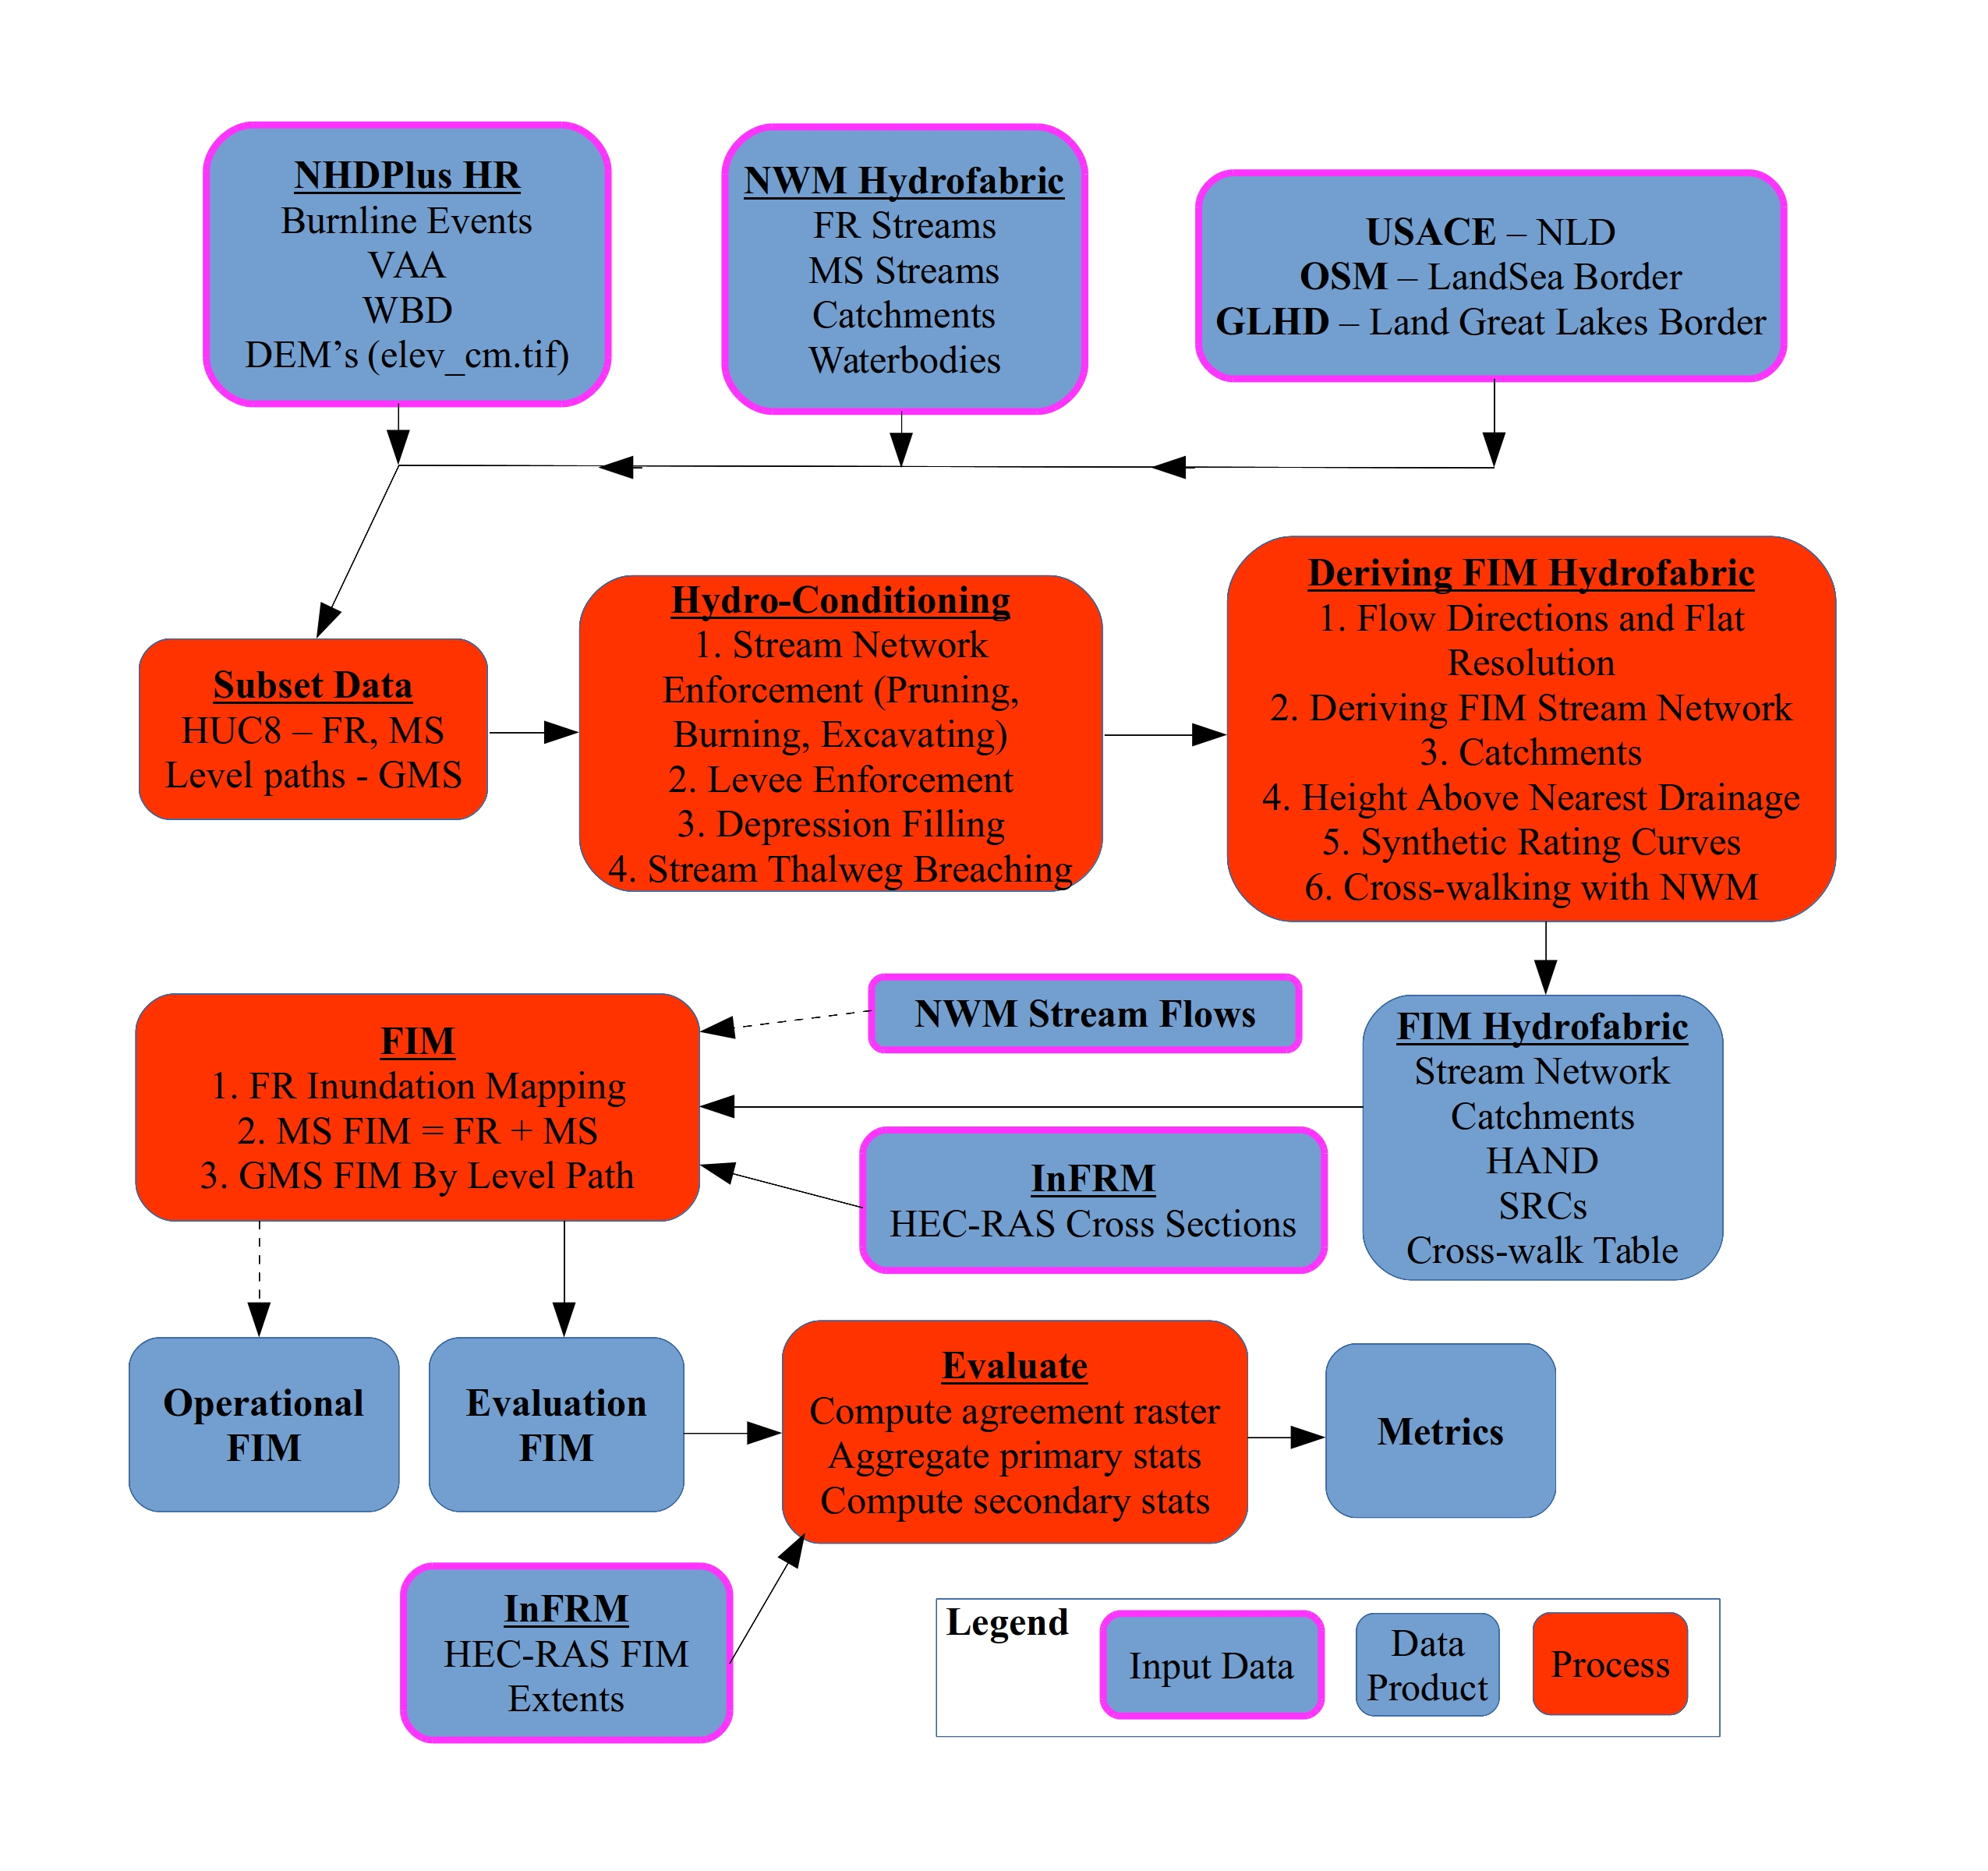
\includegraphics[scale=6.0]{figures/methods_overview.jpg}
\caption{
\DIFaddFL{Methodology overview detailing high level steps followed in the study.
The flow chart begins with the input data organized by source.
Subsetting the data into processing units depends on which model is being considered.
FR utilizes the entire NWM stream network processed at HUC8 processing areas.
MS only computes HAND using the NWM stream at or downstream of legacy forecasting points.
The resulting inundation from the MS HAND is eventually layered with the FIM from FR HAND to account for high levels of inundation contributed by the mainstem.
Generalized Mainstem (GMS) discretized NWM streams into level paths (LP) then computes HAND and the FIMs independently only to mosaic them later. 
This better accounts for multiple possible sources of fluvial inundation.
The dotted lines denote the use of NWM streamflow forecasts to produce operational FIM but not used in this study.
All acronyms used in the figure are defined in the paper.
}}
\label{fig:methods_overview}
\end{figure}
%DIF > 
%DIF > 
\DIFaddend %%%%%%%%%%%%%%%%%%%%%%%%%%%%%%%%%%%%%%%%%%%%%%%%%%%%%%%%
\subsection{Software Dependencies and Architecture}
\DIFaddbegin \label{ssec:software}
\DIFaddend %%%%%%%%%%%%%%%%%%%%%%%%%%%%%%%%%%%%%%%%%%%%%%%%%%%%%%%%
%
OWP FIM exclusively utilizes free and open source software dependencies including Python 3, GDAL, TauDEM, Geographic Resource Analysis Support System (GRASS), GNU Parallel, and MPICH \cite{python382,gdal2020,tarboton2005terrain,grass2020,tange2015gnu,amer2021mpich}.
Within the Python 3 ecosystem, many common packages are employed including but not limited to RichDEM, GeoPandas, Rasterio, Rasterstats, and Numba \cite{barnes2018richdem,jordahl2014geopandas,lam2015numba}. 
To simplify setup and enhance portability across host operating systems\DIFaddbegin \DIFadd{, }\DIFaddend OWP FIM packages all dependencies up in a Docker image \DIFdelbegin \DIFdel{(}%DIFDELCMD < \url{https://docs.docker.com/engine/install/}%%%
\DIFdel{)}\DIFdelend \DIFaddbegin \DIFadd{\mbox{%DIFAUXCMD
\cite{merkel2014docker}}\hskip0pt%DIFAUXCMD
}\DIFaddend . 
A user only needs to install Docker on their host machine and build the image from the provided recipe. 
Source code is made available for this project on GitHub \DIFdelbegin \DIFdel{\mbox{%DIFAUXCMD
\cite{inundationMapping2022}}\hskip0pt%DIFAUXCMD
. 
}%DIFDELCMD < 

%DIFDELCMD < %%%
\DIFdel{The pipeline is discretized into key areas that a user can interact with to reproduce the results of this study. 
Preprocessing acquires and prepares datasets for production of the FIM hydrofabric. 
The FIM hydrofabric is defined as the datasets required to make an inundation map from discharges including the relative elevation model (REM) or HAND grid, the catchments in vector and raster form, and the hydro-table (contains synthetic rating curves and cross-walk information).
Functionality is included to turn FIM hydrofabric and streamflows into inundation maps represented in both binary and depths.
Lastly, a test suite includes means of calculating evaluation metrics compared to a variety of preprocessed test case data.
A user should visit the }\DIFdelend \DIFaddbegin \DIFadd{where a user could consult the }\DIFaddend Readme.md page \DIFdelbegin \DIFdel{on GitHub }\DIFdelend for more information on how to acquire the datasets and reproduce the pipeline \DIFaddbegin \DIFadd{\mbox{%DIFAUXCMD
\cite{inundationMapping2022}}\hskip0pt%DIFAUXCMD
}\DIFaddend .
%
%%%%%%%%%%%%%%%%%%%%%%%%%%%%%%%%%%%%%%%%%%%%%%%%%%%%%%%%
\subsection{Datasets}
\label{ssec:datasets}
%%%%%%%%%%%%%%%%%%%%%%%%%%%%%%%%%%%%%%%%%%%%%%%%%%%%%%%%
%
Data sources used within OWP FIM are publicly available from a variety of government sources including the USGS, NWC, Federal Emergency Management Agency (FEMA), and US Army Core of Engineers (USACE) to enhance reproducibility and collaboration among government, academia, and industry.
Instructions for accessing data \DIFaddbegin \DIFadd{processed for OWP FIM }\DIFaddend are provided on the project's GitHub page via an Amazon Web Services (AWS) S3 bucket furnished by \DIFaddbegin \DIFadd{the }\DIFaddend Earth Science Information Partners (ESIP) \cite{esipData2022}.
The National Hydrography Dataset Plus High Resolution (NHDPlusHR) Beta Version is the latest hydrography dataset used for land surface hydrologic modeling in the US \cite{moore2019user}.
\DIFdelbegin \DIFdel{It is }\DIFdelend \DIFaddbegin \DIFadd{We utilized a series of data products from the NHDPlusHR including the BurnLineEvents \mbox{%DIFAUXCMD
\cite{nhdplus2022vectors}}\hskip0pt%DIFAUXCMD
, Value Added Attributes (VAA) \mbox{%DIFAUXCMD
\cite{nhdplus2022vectors}}\hskip0pt%DIFAUXCMD
, Water Boundaries (WBD) or HUC Layers \mbox{%DIFAUXCMD
\cite{nhdplus2022wbd}}\hskip0pt%DIFAUXCMD
, and the DEM elevation rasters \mbox{%DIFAUXCMD
\cite{nhdplus2022dems}}\hskip0pt%DIFAUXCMD
.
These BurnLines }\DIFaddend used in conjunction with the hydrofabric of the NWM V2.1 to help define flowlines for OWP FIM while the NWM hydrofabric is also used to define reservoirs for exclusion and catchments to cross-walk \DIFdelbegin \DIFdel{to }\DIFdelend \DIFaddbegin \DIFadd{against }\DIFaddend for forecasting purposes \DIFaddbegin \DIFadd{\mbox{%DIFAUXCMD
\cite{nwm2022hydrofabric}}\hskip0pt%DIFAUXCMD
}\DIFaddend .
For enforcing levee data\DIFdelbegin \DIFdel{into the DEMs}\DIFdelend , the USACE \DIFdelbegin \DIFdel{National Levee Database (NLD ) }\DIFdelend \DIFaddbegin \DIFadd{NLD }\DIFaddend is used to burn feature elevations \DIFaddbegin \DIFadd{into DEMs }\DIFaddend \cite{engineers2016national}.
Since NHDPlusHR datasets extend beyond land borders into sea and Great Lake regions, we used the land-sea border from OpenStreetMap (OSM) \DIFaddbegin \DIFadd{\mbox{%DIFAUXCMD
\cite{osm2021landsea} }\hskip0pt%DIFAUXCMD
}\DIFaddend and the land-lake border from Great Lakes Hydrography Dataset (GLHD) \DIFaddbegin \DIFadd{\mbox{%DIFAUXCMD
\cite{GreatLakesHydrographyDataset} }\hskip0pt%DIFAUXCMD
}\DIFaddend to exclude those areas from production of FIMs\DIFdelbegin \DIFdel{\mbox{%DIFAUXCMD
\cite{OpenStreetMap,GreatLakesHydrographyDataset}}\hskip0pt%DIFAUXCMD
}\DIFdelend .
Additionally, the Base Level Engineering (BLE) datasets within FEMA Region 6 spanning parts of \DIFdelbegin \DIFdel{9 }\DIFdelend \DIFaddbegin \DIFadd{nine }\DIFaddend states including Colorado, New Mexico, Texas, Oklahoma, Kansas, Arkansas, Louisiana, Missouri and Mississippi at two recurrence intervals, 1\% (100 year \DIFaddbegin \DIFadd{or yr}\DIFaddend ) and 0.2\% (500 year \DIFaddbegin \DIFadd{or yr}\DIFaddend ), are used \DIFdelbegin \DIFdel{as }\DIFdelend \DIFaddbegin \DIFadd{for }\DIFaddend validation in this study and furnished by the Interagency Flood Risk Management (InFRM) consortium \cite{fema2021base,fema2021estimated}. 
These BLE datasets are provided at the watershed scale (HUC8) utilizing best available \DIFdelbegin \DIFdel{simulations and DEMs }\DIFdelend \DIFaddbegin \DIFadd{DEMs and simulations from the Hydrologic Engineering Center's River Analysis System (HEC-RAS) model \mbox{%DIFAUXCMD
\cite{us2022hydrologic}}\hskip0pt%DIFAUXCMD
}\DIFaddend .
The full input datasets presented by source are listed in Table \ref{tab:data}.
%
\DIFdelbegin %DIFDELCMD < \begin{table}
%DIFDELCMD < %%%
\DIFdelendFL \DIFaddbeginFL \begin{sidewaystable}
\DIFaddendFL \caption{Data sources, names, \DIFdelbeginFL \DIFdelFL{and }\DIFdelendFL descriptions\DIFaddbeginFL \DIFaddFL{, and citations}\DIFaddendFL .}
\label{tab:data}
\centering
\DIFdelbeginFL %DIFDELCMD < \begin{tabular}{|p{2cm}|p{4cm}|p{8cm}|}
%DIFDELCMD < %%%
\DIFdelendFL \DIFaddbeginFL \begin{tabular}{|p{1.75cm}|p{4cm}|p{11cm}|p{5cm}|}
\DIFaddendFL %\begin{tabular}{l c c}
\hline
Source & Name & Description \DIFaddbeginFL & \DIFaddFL{Citations}\DIFaddendFL \\
\hline
USGS & NHDPlusHR BurnLineEvents & Stream lines used by \DIFdelbeginFL \DIFdelFL{NHDPlus HR }\DIFdelendFL \DIFaddbeginFL \DIFaddFL{NHDPlusHR }\DIFaddendFL for hydro-enforcement\DIFaddbeginFL \DIFaddFL{. }& \DIFaddFL{\mbox{%DIFAUXCMD
\cite{nhdplus2022vectors} }\hskip0pt%DIFAUXCMD
}\DIFaddendFL \\
\hline
USGS & NHDPlusHR Value-Added Attributes & Database of additional attributes associated with the BurnLineEvents that enhance navigation, analysis, and display\DIFaddbeginFL \DIFaddFL{. }& \DIFaddFL{\mbox{%DIFAUXCMD
\cite{nhdplus2022vectors} }\hskip0pt%DIFAUXCMD
}\DIFaddendFL \\
\hline
USGS & NHDPlusHR DEM & DEM used for \DIFdelbeginFL \DIFdelFL{NHDPlus HR }\DIFdelendFL \DIFaddbeginFL \DIFaddFL{NHDPlusHR }\DIFaddendFL at 1/3 arc-second (10 m) spatial resolution and vertical units in centimeters\DIFaddbeginFL \DIFaddFL{. }& \DIFaddFL{\mbox{%DIFAUXCMD
\cite{nhdplus2022dems} }\hskip0pt%DIFAUXCMD
}\DIFaddendFL \\
\hline
\DIFaddbeginFL \DIFaddFL{USGS }& \DIFaddFL{NHDPlusHR WBD }& \DIFaddFL{Water Boundaries (WBD) or HUCs used for spatial processing units. }& \DIFaddFL{\mbox{%DIFAUXCMD
\cite{nhdplus2022wbd} }\hskip0pt%DIFAUXCMD
}\\
\hline
\DIFaddendFL NOAA-OWP & NWM Streams & Stream network center lines used by NWM for routing and forecasting \DIFdelbeginFL \DIFdelFL{. }\DIFdelendFL \DIFaddbeginFL \DIFaddFL{adapted from NHDPlus V2 NHDFlowline\_Network feature class. }& \DIFaddFL{\mbox{%DIFAUXCMD
\cite{nwm2022hydrofabric} }\hskip0pt%DIFAUXCMD
}\DIFaddendFL \\
\hline
NOAA-OWP & NWM Catchments & Surface drainage area corresponding to each reach in the NWM \DIFdelbeginFL \DIFdelFL{. }\DIFdelendFL \DIFaddbeginFL \DIFaddFL{adapted from NHDPlus V2 Catchment feature class. }& \DIFaddFL{\mbox{%DIFAUXCMD
\cite{nwm2022hydrofabric} }\hskip0pt%DIFAUXCMD
}\DIFaddendFL \\
\hline
NOAA-OWP & NWM Waterbodies & Waterbodies considered by the NWM as reservoirs or lakes \DIFdelbeginFL \DIFdelFL{. }\DIFdelendFL \DIFaddbeginFL \DIFaddFL{adapted from NHDPlus V2 NHDWaterbody feature class. }& \DIFaddFL{\mbox{%DIFAUXCMD
\cite{nwm2022hydrofabric} }\hskip0pt%DIFAUXCMD
}\DIFaddendFL \\
\hline
USACE & NLD & Levee database of locations and elevations\DIFaddbeginFL \DIFaddFL{. }& \DIFaddFL{\mbox{%DIFAUXCMD
\cite{engineers2016national} }\hskip0pt%DIFAUXCMD
}\DIFaddendFL \\
\hline
OSM & Land-Sea Border & Border of land and sea. \DIFaddbeginFL & \DIFaddFL{\mbox{%DIFAUXCMD
\cite{osm2021landsea} }\hskip0pt%DIFAUXCMD
}\DIFaddendFL \\
\hline
GLHD & Land-Great Lakes Border & Border of land and Great Lakes. \DIFaddbeginFL & \DIFaddFL{\mbox{%DIFAUXCMD
\cite{GreatLakesHydrographyDataset} }\hskip0pt%DIFAUXCMD
}\DIFaddendFL \\
\hline
InFRM & Cross-Sections & HEC-RAS \DIFdelbeginFL \DIFdelFL{1-D }\DIFdelendFL \DIFaddbeginFL \DIFaddFL{1D }\DIFaddendFL cross-sections used for modeling in BLE datasets. Includes discharges for 1\% and 0.2\% recurrence interval events. \DIFaddbeginFL & \DIFaddFL{\mbox{%DIFAUXCMD
\cite{fema2021estimated} }\hskip0pt%DIFAUXCMD
}\DIFaddendFL \\
\hline
InFRM & Flood Inundation Extents & Inundation depths produced by InFRM BLE HEC-RAS 1D for 1\% and 0.2\% recurrence interval events. \DIFaddbeginFL & \DIFaddFL{\mbox{%DIFAUXCMD
\cite{fema2021estimated} }\hskip0pt%DIFAUXCMD
}\DIFaddendFL \\
\hline
\end{tabular}
\DIFdelbeginFL %DIFDELCMD < \end{table}
%DIFDELCMD < %%%
\DIFdelend %DIF > \end{table}
\DIFaddbegin \end{sidewaystable}
\DIFaddend %
Areas with all the required data (from the NWM and the USGS) are labeled as the FIM domain which includes 2,188 HUC8s for the FR and GMS networks and 1,604 HUC8s for the MS method. 
These methods will be explained \DIFdelbegin \DIFdel{more }\DIFdelend \DIFaddbegin \DIFadd{in more detail }\DIFaddend later.
An enhancement of OWP FIM over previous HAND based FIM versions is the support for Hawaii and Puerto Rico which \DIFaddbegin \DIFadd{are expansion domains in }\DIFaddend the NWM V2\DIFaddbegin \DIFadd{.0 and V2}\DIFaddend .1\DIFdelbegin \DIFdel{will cover}\DIFdelend \DIFaddbegin \DIFadd{, respectively}\DIFaddend .
%
%%%%%%%%%%%%%%%%%%%%%%%%%%%%%%%%%%%%%%%%%%%%%%%%%%%%%%%%
\subsection{Hydro-conditioning}
\label{ssec:hydro_conditioning}
%%%%%%%%%%%%%%%%%%%%%%%%%%%%%%%%%%%%%%%%%%%%%%%%%%%%%%%%
%
The DEM is subject to a series of hydro-conditioning procedures to enhance its suitability for riverine flood inundation mapping \DIFaddbegin \DIFadd{with HAND}\DIFaddend . 
These techniques are specific for making OWP FIM and differ from the conditioning methods used by the NHDPlusHR Beta \cite{moore2019user}.
HAND inherently requires all areas eligible for inundation to drain to the designated drainage network\DIFdelbegin \DIFdel{so }\DIFdelend \DIFaddbegin \DIFadd{.
So to satisfy this requirment, }\DIFaddend DEMs must undergo significant manipulation\DIFdelbegin \DIFdel{to make this the case}\DIFdelend .
In other words, all areas within a given processing unit for HAND must have monotonically decreasing elevations \DIFdelbegin \DIFdel{if we wish to have them be eligble }\DIFdelend \DIFaddbegin \DIFadd{to enable eligiblity }\DIFaddend for flooding.
Hydro-conditioning is implemented to obtain many objectives including enforcing the location of hydrologically relevant features such as flowlines, lakes, or drainage divides whether natural or anthropogenic. 
It can also be used to simulate more accurate bathymetry which is not accounted for in the 10 m DEM \cite{gesch2002national}.

Specifically within the context of OWP FIM, the hydro-conditioning operations that take place in sequential order are presented. 
Prior to any hydro-conditioning, all input datasets must be subset from their original spatial domain scales into the processing units of size HUC8. 
The subsetting is done by spatial query for the cases of the levees, DEM, and NWM hydrofabric while the NHDPlusHR BurnLineEvents are subset via attribute query for the given reach code's membership in the processing unit.
Hydro-conditioning raster operations take place on buffered boundary definitions to avoid edge contamination and effects \cite{lindsay2013measuring}. 
%
%%%%%%%%%%%%%%%%%%%%%%%%%%%%%%%%%%%%%%%%%%%%%%%%%%%%%%%%
\subsubsection{Stream Network Enforcement} 
\label{ssec:stream_network_enforcment}
%
The location of the stream network is enforced to ensure general agreement with \DIFdelbegin \DIFdel{established stream networks}\DIFdelend \DIFaddbegin \DIFadd{the NWM network which is used for forecasting the streamflow inputs}\DIFaddend .
The NHDPlusHR Beta \DIFdelbegin \DIFdel{Burnline Event }\DIFdelend \DIFaddbegin \DIFadd{BurnLineEvent }\DIFaddend layer is used to enforce stream locations in the NHDPlusHR workflow \DIFaddbegin \DIFadd{and best agrees with thalweg locations in the DEM used }\DIFaddend so it is also used here for hydro-enforcement \cite{moore2019user}. 
\DIFaddbegin 

\DIFaddend However, to better match the drainage density of the NWM \DIFaddbegin \DIFadd{FR }\DIFaddend V2.1 stream network\DIFaddbegin \DIFadd{, }\DIFaddend which is based on the NHDPlus \DIFdelbegin \DIFdel{Medium Resolution, the Burnline Events }\DIFdelend \DIFaddbegin \DIFadd{V2, the BurnlineEvents }\DIFaddend are pruned utilizing a nearest neighbor search around the NWM flowlines.
\DIFaddbegin \DIFadd{Headwater points are first derived for the NWM FR V2.1.
}\DIFaddend For every NWM headwater \DIFdelbegin \DIFdel{segment a headwater pointis derived and linearly interpolated to the nearest Burnline Event segment.
Burnline Event headwater segments are split at the adjusted headwater point to match NWM flowlines}\DIFdelend \DIFaddbegin \DIFadd{point, the nearest NHDPlusHR point is selected and placed into a set while those excluded are discarded.
Only the nearest point on the NHDPlusHR is used so any portion of the NHDPlusHR network upstream of this nearest point is discarded to avoid extending inundation too far above the modeling domain.
The points in this nearest neighbor set are then traversed downstream.
Any headwater portion in the NHDPlusHR or any other stream not traversed are pruned away to better match the resolution and spatial locations of the NWM stream network and its headwater points}\DIFaddend .
The resulting pruned \DIFdelbegin \DIFdel{NHD stream network is what }\DIFdelend \DIFaddbegin \DIFadd{NHDPlusHR stream network }\DIFaddend gets hydro-enforced in subsequent operations.
This procedure is best illustrated in Figure \ref{fig:stream_density_pruning} which shows that the pruned \DIFdelbegin \DIFdel{NHD }\DIFdelend \DIFaddbegin \DIFadd{NHDPlusHR }\DIFaddend network corresponds to the \DIFdelbegin \DIFdel{full density NHD network at }\DIFdelend \DIFaddbegin \DIFadd{NHDPlusHR network at or downstream of }\DIFaddend NWM V2.1 headwater locations only. 
Additionally, the NHDPlusHR pruned headwaters are later used for seeding a new FIM drainage network that best agrees with the DEM after all hydro-conditioning takes place.
%DIF < 
\DIFdelbegin %DIFDELCMD < \begin{figure}[h!]
%DIFDELCMD < \centering
%DIFDELCMD < 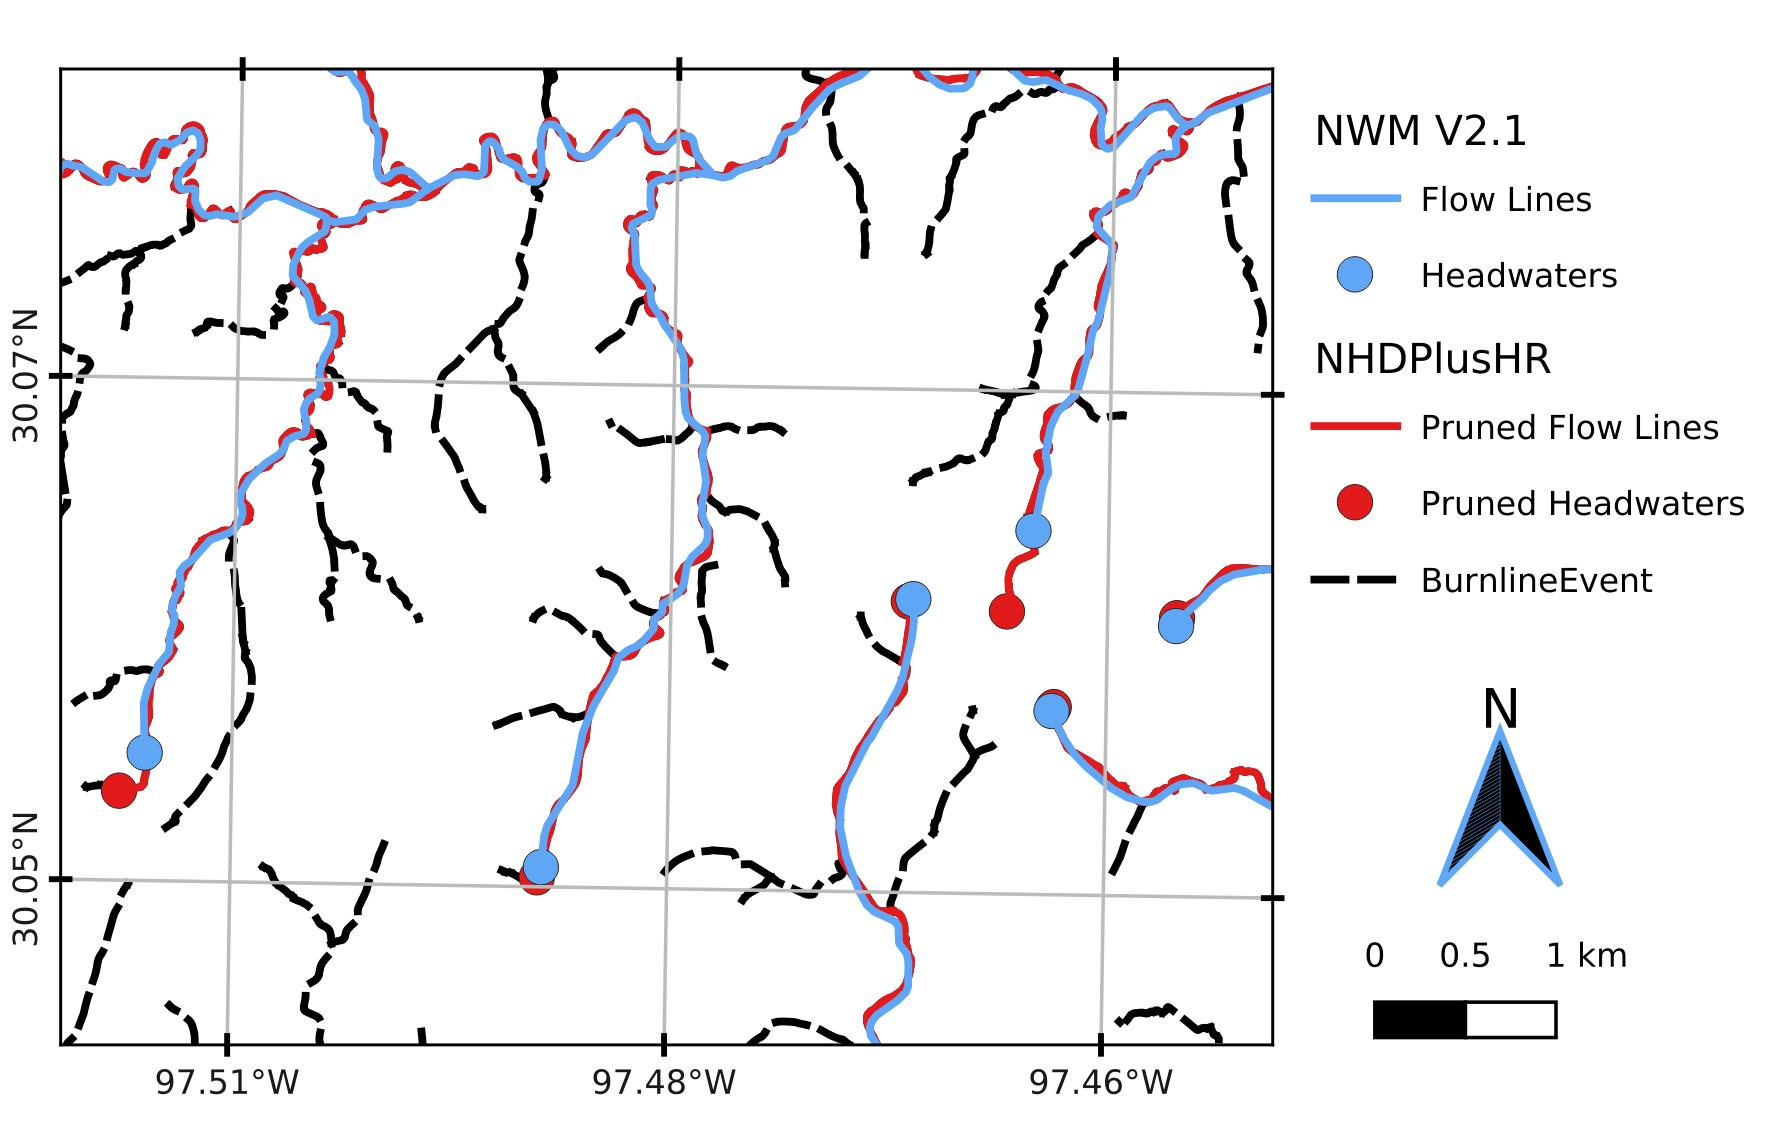
\includegraphics[scale=1.0]{figures/headwaters.jpg}
%DIFDELCMD < %%%
%DIFDELCMD < \caption{%
{%DIFAUXCMD
\DIFdelFL{Pruning of NHDPlus HR Beta Burnline Events (dotted black) to NWM V2.1 stream density (blue) using nearest neighbor selection and linear interpolation. Resulting stream network (red) matches the drainage density of NWM V2.1 while corresponding spatially with the NHDPlusHR Burnline Events.}}
%DIFAUXCMD
%DIFDELCMD < \label{fig:stream_density_pruning}
%DIFDELCMD < \end{figure}
%DIFDELCMD < %%%
%DIF < 
\DIFdelend This results in a stream network that has the same density as the NWM V2.1 flowline network but utilizes the locations of the NHDPlusHR Beta BurnLineEvents. 
%DIF > 
\DIFaddbegin \begin{figure}[H]
\centering
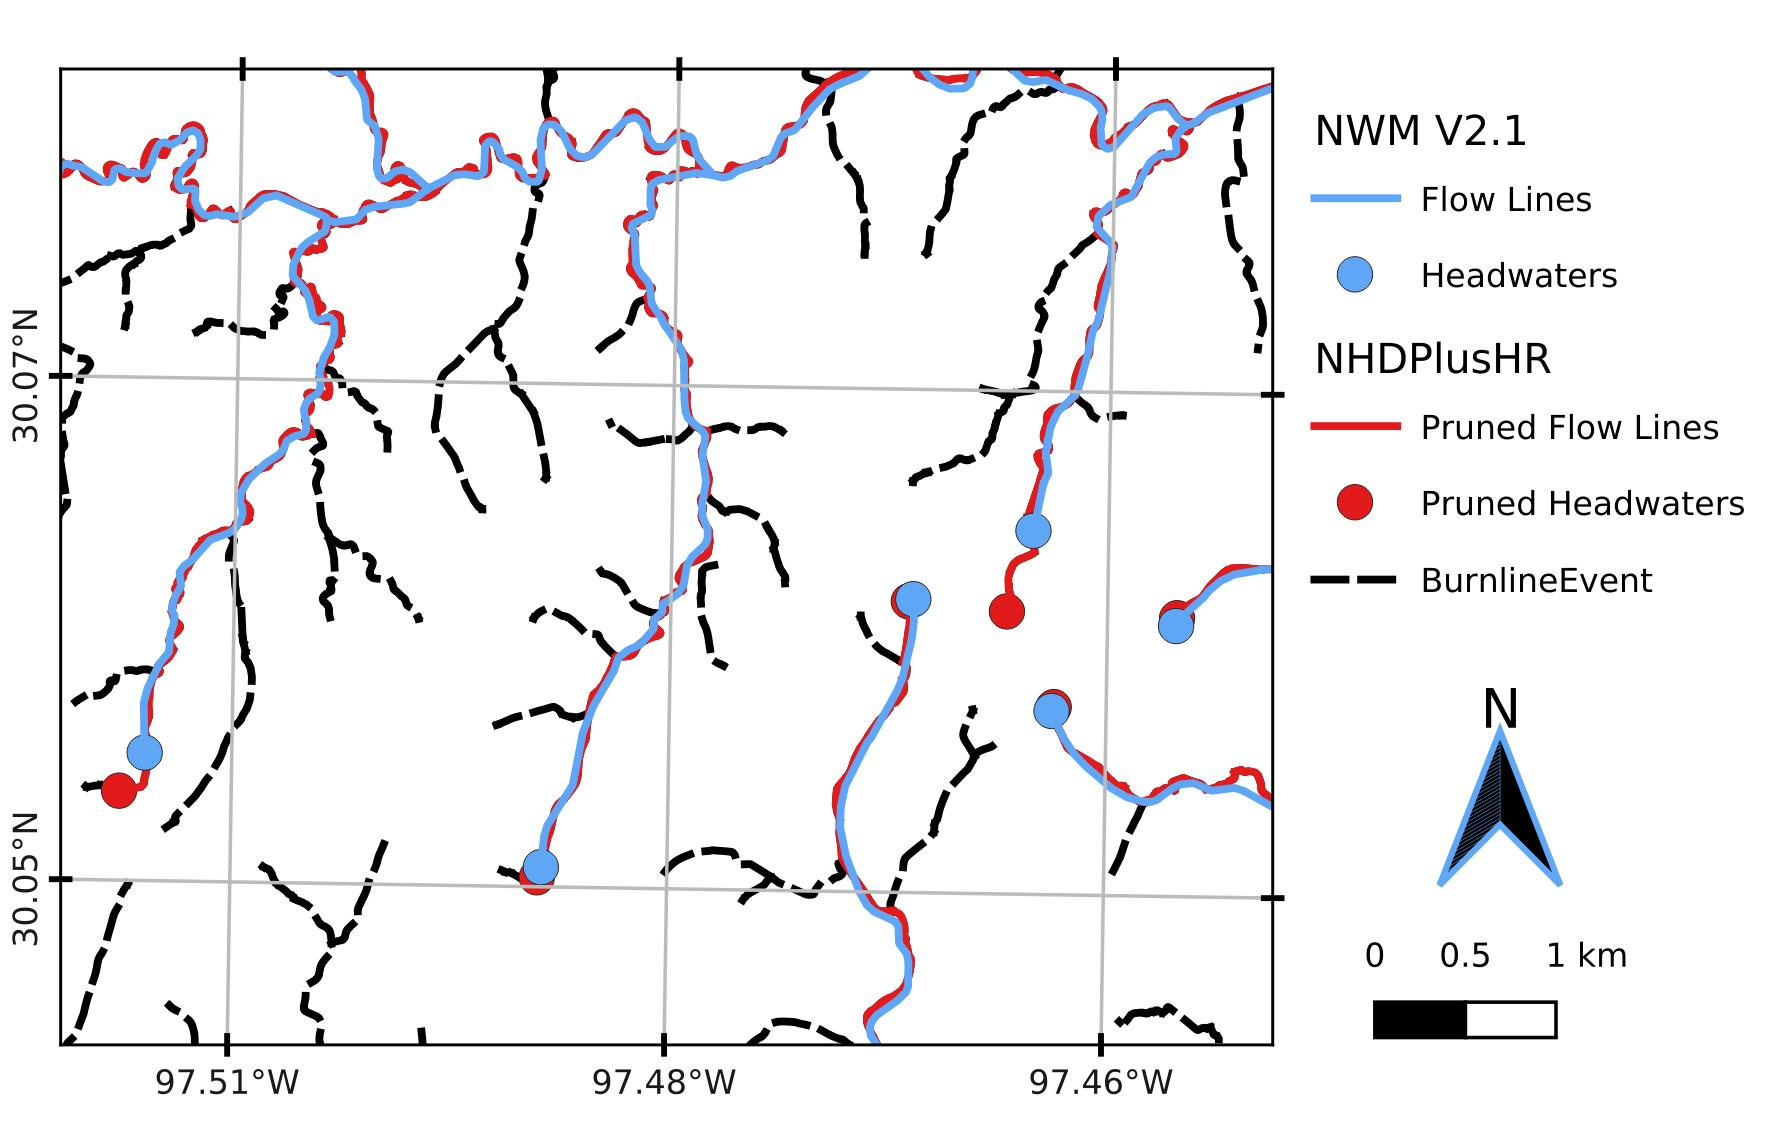
\includegraphics[scale=1.0]{figures/headwaters.jpg}
\caption{\DIFaddFL{This figure illustrates some of the datasets that result from the pruning of NHDPlusHR Beta BurnlineEvents (dotted black) to the stream density of the NWM FR V2.1 density (blue).
The stream network used for forecasting, NWM FR V2.1, is of lower stream density than that of the NHDPlusHR which has better agreement with the thalweg locations in the DEM used.
Thus, we opt to prune the NHDPlusHR network to match the general location and density of the NWM network.
The nearest neighbor segment in the NHDPlusHR of each NWM headwater locations and the nearest point on that segment is determined to match the closest point to that of the NWM headwater.
These points are then traversed downstream and any segments not traversed are pruned away.
The resulting stream network (red) matches the drainage density of NWM V2.1 while corresponding spatially with the NHDPlusHR BurnlineEvents.}}
\label{fig:stream_density_pruning}
\end{figure}
%DIF > 
\DIFaddend 

The pruned stream network is then utilized to hydro-enforce the DEM with a methodology developed by \citeA{hellweger1997agree} known as the AGREE DEM Surface Reconditioning System. 
The AGREE algorithm seeks to burn artificially deep thalweg elevations by a uniform value known as sharp drop. 
The modification continues by excavating an area of a given buffer distance from the thalweg by a depth proportional to the distance from the channel given by the smooth drop \DIFaddbegin \DIFadd{and buffer distance}\DIFaddend . 
The resulting enforcement of the thalweg and general bathymetric region results in a cross-section resembling \DIFdelbegin \DIFdel{a trapezoidal }\DIFdelend \DIFaddbegin \DIFadd{an inverted triangular notch }\DIFaddend shape with a significantly lower elevation along the thalweg line only.
In total, the AGREE algorithm requires three parameters including the buffer distance, smooth drop, and sharp drop \DIFdelbegin \DIFdel{. 
}\DIFdelend \DIFaddbegin \DIFadd{which were set to fixed values of 70 m, 1000 m, and 10 m, respectively, but available to the user via the parameter file.
While the values for these parameters are critical to the inundation extents produced, especially for lower flow rates where bathymetric information has more influence, finding their optimal values for OWP FIM was not done since it was out of the main scientific scope of this article.
}\DIFaddend Using the AGREE method as opposed to simple thalweg burning techniques helps prevent distortions in the delineation of streams as well as the catchment boundaries \cite{saunders1995grid,saunders1996gis,mizgalewicz1996modeling,hellweger1997agree,quenzer1998gis,baker2006comparison}.
\citeA{baker2006comparison} noted AGREE produced satisfactory results when compared to other enforcement \DIFaddbegin \DIFadd{techniques }\DIFaddend especially when computational costs are considered. 
Downsides to the technique include the possibility of exhibiting parallel streams where the burned stream and real stream are both represented \cite{hellweger1997agree,saunders1999preparation} and some distortion of the catchment boundaries can also be observed \cite{saunders1999preparation,saunders1996gis}.
Some of these drawbacks are \DIFdelbegin \DIFdel{later }\DIFdelend addressed by additional conditioning techniques \DIFaddbegin \DIFadd{applied }\DIFaddend later on.
%
%%%%%%%%%%%%%%%%%%%%%%%%%%%%%%%%%%%%%%%%%%%%%%%%%%%%%%%%
\subsubsection{Levee Enforcement}
%
\DIFdelbegin \DIFdel{The DEM}\DIFdelend \DIFaddbegin \DIFadd{Coarse DEM's }\DIFaddend at 10 m\DIFdelbegin \DIFdel{resolution lacks }\DIFdelend \DIFaddbegin \DIFadd{, 30 m, and higher resolutions can lack }\DIFaddend sufficient representation of fine grain features such as embankments, \DIFdelbegin \DIFdel{floodwalls}\DIFdelend \DIFaddbegin \DIFadd{flood walls}\DIFaddend , and closure structures \DIFaddbegin \DIFadd{\mbox{%DIFAUXCMD
\cite{arundel2018assimilation,dobbs2010evaluation,wang2005comparison,sanders2007evaluation}}\hskip0pt%DIFAUXCMD
}\DIFaddend .
In order to better represent the influences of these features upon hydraulics and inundation extents, the National Levee Database (NLD) published by USACE was used to enforce elevations within the \DIFdelbegin \DIFdel{10 m }\DIFdelend \DIFaddbegin \DIFadd{1/3 arc-second }\DIFaddend DEM.
The elevations found in the NLD are burned \DIFdelbegin \DIFdel{into }\DIFdelend \DIFaddbegin \DIFadd{onto }\DIFaddend the DEM if those elevations were found to exceed those already in place.
%
%%%%%%%%%%%%%%%%%%%%%%%%%%%%%%%%%%%%%%%%%%%%%%%%%%%%%%%%
\subsubsection{Depression Filling}
\label{sssec:depression_filling}
%
Local depressions are naturally occurring features of a DEM but must be addressed if a connected drainage network with continuous catchments are to be derived for flood modeling purposes \DIFdelbegin \DIFdel{.
The }\DIFdelend \DIFaddbegin \DIFadd{with HAND.
The partially }\DIFaddend conditioned DEM was removed of depressions by filling areas with pits while preserving the stream and levee information previously enforced.
Priority-Flood developed by \citeA{barnes2014priority} is an algorithm for filling said depressions and shown to have improved performance over early works in the field by \citeA{jenson1988extracting} implemented in \citeA{tarboton2005terrain} as well as \citeA{planchon2002fast}.
The depression filling algorithm used in our pipeline is a Priority-Flood variant developed by \cite{zhou2016efficient} with enhanced single-thread performance and a time complexity of O(n log n) for floating point grids.
This performance was enabled by limiting the processing queue with a region-growing method to exclude many of the slope cells \cite{zhou2016efficient}.
The depression \DIFaddbegin \DIFadd{filling }\DIFaddend technique employed here does leave the existence of flat regions where pits \DIFdelbegin \DIFdel{existed a prior }\DIFdelend \DIFaddbegin \DIFadd{previously existed }\DIFaddend thus later requiring the need for resolving these flats.
The enhanced variant of Priority-Flood is implemented and made available by \citeA{barnes2018richdem} and \citeA{zhou2015filldem}.
%
%%%%%%%%%%%%%%%%%%%%%%%%%%%%%%%%%%%%%%%%%%%%%%%%%%%%%%%%
\subsubsection{Stream Thalweg Elevation Conditioning}
\label{sssec:stream_thalweg_elevation_conditioning}
%
Thalweg elevations are critical components of relative elevation based inundation mapping thus much is performed to ensure the best available, monotonically decreasing\DIFaddbegin \DIFadd{, }\DIFaddend elevations are derived prior to \DIFaddbegin \DIFadd{the }\DIFaddend normalizing of elevations.
\DIFdelbegin \DIFdel{In order to }\DIFdelend \DIFaddbegin \DIFadd{Work on the AGREE DEM method from several authors have illustrated that the AGREE DEM method does not }\DIFaddend prevent situations where the burned thalweg and the thalweg endemic to the DEM run parallel to one another \DIFaddbegin \DIFadd{\mbox{%DIFAUXCMD
\cite{hellweger1997agree,baker2006comparison,saunders1999preparation,saunders1996gis,quenzer1998gis,saunders1995grid}}\hskip0pt%DIFAUXCMD
.
These works observe that the artificial elevations enforced by the hydrographically based stream network and AGREE DEM disagree with those naturally occurring in the native DEM.
In order to mitigate this documented issue}\DIFaddend , the normalized excavation algorithm \cite{saunders1999preparation} is used to seek a zonal (nearest neighbor) elevation minimum \DIFaddbegin \DIFadd{on the original, unconditioned DEM }\DIFaddend for each thalweg pixel. 
Each zone is defined as the thalweg's pixel nearest neighborhood within a maximum distance of 50 m.
The zonal minimum is computed for each thalweg pixel zone and the minimum is used to replace the existing thalweg elevation value.
\DIFaddbegin \DIFadd{This step essentially enforces an estimate of the native DEM thalweg elevations onto the sharp drop enforced thalweg elevations from the AGREE procedure.
}\DIFaddend 

The next step involves conditioning these local minimums along the thalweg to enforce monotonically decreasing thalweg elevations for FIM.
\citeA{garousi2019terrain} proposed an algorithm that \DIFdelbegin \DIFdel{traverses stream thalweg pixels }\DIFdelend \DIFaddbegin \DIFadd{breaches stream thalweg pixel elevations }\DIFaddend in a depth first manner\DIFdelbegin \DIFdel{starting with adding all the headwater pixels to a queue. 
The connectivity of the thalweg pixels is defined by the D-8 flow directions further discussed in Section \ref{ssec:flow_direction_and_flat_resolution}.
At every thalweg pixel, the minimum elevation among itself and its upstream contributing thalweg pixels is taken as shown in Equation \ref{eq:thalweg_breach},
%DIF < 
}%DIFDELCMD < \begin{linenomath*}
%DIFDELCMD < %%%
\begin{displaymath}
\DIFdel{\label{eq:thalweg_breach}
\textbf{D}[x] = \min_{y\ drains\ to\ x} }{\DIFdel{(\ \textbf{D}[x]\ ,\ \textbf{D}[y]\ )}}
\DIFdel{}\end{displaymath}%DIFAUXCMD
%DIFDELCMD < \end{linenomath*}
%DIFDELCMD < %%%
%DIF < 
\DIFdel{, in which }\textbf{\DIFdel{D}} %DIFAUXCMD
\DIFdel{represents the array of thalweg adjusted elevations indexed by x and y where by y is upstream of x. 
When a pixel's upstream neighbors are all evaluated, the downstream pixel is added into the queue thus the depth first traversal of the drainage network.
This procedure enforces the location of streams and ensures that thalweg elevations are hydrologically correct which yielded a 7\% improvement in }\DIFdelend \DIFaddbegin \DIFadd{. 
This procedure was found to increase the }\DIFaddend Critical Success Index (CSI) \DIFdelbegin \DIFdel{per an evaluation for an event in 2017 on the Malad river \mbox{%DIFAUXCMD
\cite{garousi2019terrain}}\hskip0pt%DIFAUXCMD
}\DIFdelend \DIFaddbegin \DIFadd{of resulting FIMs from HAND and is employed in OWP FIM to enforce monotonically decreasing elevations with thalweg pixel networks}\DIFaddend .
%
%%%%%%%%%%%%%%%%%%%%%%%%%%%%%%%%%%%%%%%%%%%%%%%%%%%%%%%%
\subsection{Deriving FIM Hydrofabric}
\label{ssec:deriving_fim_hydrofabric}
%%%%%%%%%%%%%%%%%%%%%%%%%%%%%%%%%%%%%%%%%%%%%%%%%%%%%%%%
%
The FIM Hydrofabric is defined here as the collection of geospatial datasets that are used for converting NWM discharges into inundation extents.
\DIFaddbegin \DIFadd{These datasets include the HAND or relative elevation model (REM) raster, reach-level catchments raster/polygons, DEM-derived streamlines, SRCs, and cross-walk table.
The following sub-sections describe how the subset and hydro-enforced geospatial datasets are converted into the FIM hydrofabric.
}\DIFaddend %
%%%%%%%%%%%%%%%%%%%%%%%%%%%%%%%%%%%%%%%%%%%%%%%%%%%%%%%%
\subsubsection{Flow Directions and Flats Resolution}
\label{ssec:flow_direction_and_flat_resolution}
%
To facilitate the generation of a connected stream network and its associated catchments from the conditioned DEM, the depression-filled DEM is used to derive connectivity in the form of D-8 flow directions.
D-8 seeks to allocate a drainage direction for every pixel based on the adjacent eight pixel neighborhood with the steepest slope \cite{o1984extraction}.
The horizontal component of slope is defined as one for the \DIFdelbegin \DIFdel{4 }\DIFdelend \DIFaddbegin \DIFadd{four }\DIFaddend neighboring pixels in the main cardinal directions while the intercardinal pixels are designated a horizontal component of $\sqrt{2}$ \DIFdelbegin \DIFdel{. 
The flow direction is encoded as integers 1 through 8 corresponding with the cardinal direction East as 1 and continuing counter-clockwise to the Southeast direction as 8. 
}\DIFdelend \DIFaddbegin \DIFadd{by means of the Pythagorean theorem. 
}\DIFaddend Flow directions are derived for non-depression filled regions trivially with the above procedure but to define connectivity for every grid cell the remaining flats corresponding to \DIFdelbegin \DIFdel{depression filled }\DIFdelend \DIFaddbegin \DIFadd{depression-filled }\DIFaddend cells must be resolved.

Flat resolution from flats endemic to the DEM or from depression filled regions is a costly, non-trivial procedure which was originally addressed by \citeA{garbrecht1997assignment} \DIFaddbegin \DIFadd{where flats are resolved by incrementing elevations iteratively}\DIFaddend .
Software implementations have developed means to partition the problem and resolve flats iteratively with communication across processes \cite{tarboton2009generalized,tesfa2011extraction,wallis2009parallel,tarboton2005terrain}.
The excessive iteration and communication leads to poor computational performance which motivated further work on how to optimize flat resolution \cite{survila2016scalable,barnes2014efficient}.
\DIFdelbegin \DIFdel{Specifically the work by \mbox{%DIFAUXCMD
\citeA{survila2016scalable} }\hskip0pt%DIFAUXCMD
enables the use of parallel processing and made smoother catchments from our informal experience than those from \mbox{%DIFAUXCMD
\citeA{barnes2014efficient}}\hskip0pt%DIFAUXCMD
.
By processing flats local to each partition separately from flats shared with other partitions, the accelerated flat resolution algorithm demonstrated an average speed up of 468x when compared to prior implementations \mbox{%DIFAUXCMD
\cite{survila2016scalable}}\hskip0pt%DIFAUXCMD
.
}\DIFdelend \DIFaddbegin \DIFadd{The established literature in this niche field of hydrology discusses how prevalent flats can be in given study areas and how difficult the problem is from both computational and hydrologic stand-points \mbox{%DIFAUXCMD
\cite{garbrecht1997assignment,tarboton2009generalized,tarboton2005terrain,survila2016scalable,barnes2014efficient,tesfa2011extraction,wallis2009parallel}}\hskip0pt%DIFAUXCMD
.
}\DIFaddend OWP FIM utilized a CyberGIS implementation of the D-8 flow direction algorithm with the accelerated resolution of flats \DIFaddbegin \DIFadd{which we found to be very efficient and effective }\DIFaddend \cite{survila2016scalable,cybergis2016}.
%
%%%%%%%%%%%%%%%%%%%%%%%%%%%%%%%%%%%%%%%%%%%%%%%%%%%%%%%%
\subsubsection{Deriving FIM Stream Network}
\label{sssec:deriving_fim_stream_network}
%
The derivations of relative elevations and catchments from the newly conditioned DEM involves re-deriving a new\DIFaddbegin \DIFadd{, DEM based, }\DIFaddend FIM stream network. 
The FIM stream network is of similar drainage density as the NWM V2.1 network \DIFdelbegin \DIFdel{but }\DIFdelend \DIFaddbegin \DIFadd{and }\DIFaddend fully converges at all junctions leaving no divergences in the network.
This is accomplished by using the seed points generated from the stream network enforcement process (Section \ref{ssec:stream_network_enforcment}).
These seeds points are \DIFaddbegin \DIFadd{pruned }\DIFaddend headwater locations of the NHDPlusHR Beta \DIFdelbegin \DIFdel{Burnline Events }\DIFdelend \DIFaddbegin \DIFadd{BurnlineEvents }\DIFaddend layer that spatially correspond to the headwater definitions in the stream network of the NWM V2.1.
Feeding the seed points and previously computed flow directions into flow accumulation methods \cite{wallis2009parallel,tarboton1997new,tarboton2005terrain} yields a stream link accumulation raster that can be converted to a vector file for further processing.
\DIFaddbegin 

\DIFaddend Each stream link in this derived FIM stream network is split into equidistant reaches \DIFaddbegin \DIFadd{of 1.5 km in length which is a user exposed parameter}\DIFaddend .
Stream links are defined here as segments of rivers discretized by junctions with other NWM river segments.
Stream links are then further segmented at NWM lakes and HUC8 boundaries.
Discretizing at NWM lakes isolates reaches and catchments associated with lakes and reservoirs to avoid mapping them using the Manning's equation and could potentially enable volume based mapping in the future as a feature enhancement.
Based on previous research, splitting each remaining stream link into equidistant reaches not to exceed a parameterized value of 1.5 km helps improve \DIFdelbegin \DIFdel{synthetic rating curve }\DIFdelend \DIFaddbegin \DIFadd{SRC }\DIFaddend and mapping skill \cite{garousi2019terrain,godbout2019error,zheng2018geoflood}.
Small reaches can lead to unrealistic variances in channel geometries while oversized reaches can lead to grouping too much slope variance into one \DIFdelbegin \DIFdel{discretation }\DIFdelend \DIFaddbegin \DIFadd{discretization }\DIFaddend of the stream network.
Short stream segments that are introduced as a result of forced network breaks due to reservoir, levee, or HUC boundaries \DIFdelbegin \DIFdel{inherent the synthetic rating curve }\DIFdelend \DIFaddbegin \DIFadd{inherit the SRC }\DIFaddend properties of the upstream or downstream segment, depending on the topology.
Section \ref{sssec:synthetic_rating_curve} details the derivation of the \DIFdelbegin \DIFdel{synthetic rating curves }\DIFdelend \DIFaddbegin \DIFadd{SRC }\DIFaddend and the dependence on channel length. 
Additionally every reach (and later catchment) is assigned a globally unique identifier based on the \DIFdelbegin \DIFdel{HUC 8 }\DIFdelend \DIFaddbegin \DIFadd{HUC8 }\DIFaddend membership.
This stream network is important since it drives the HAND calculation and derivation of catchments.
%
%%%%%%%%%%%%%%%%%%%%%%%%%%%%%%%%%%%%%%%%%%%%%%%%%%%%%%%%
\subsubsection{Catchments}
\label{sssec:catchments}
%
Catchments were derived using the D8 connectivity established by \citeA{o1984extraction}.
Outlet points are set at the pixel center points of the delineated stream lines explained in Section \ref{sssec:deriving_fim_stream_network}.
The outlets act as root nodes in a tree structure and the connectivity is traversed to derive the contributing\DIFdelbegin \DIFdel{area for each gage}\DIFdelend \DIFaddbegin \DIFadd{, nearest drainage region for each outlet point}\DIFaddend .
Two sets of catchments are derived, one \DIFdelbegin \DIFdel{of which assigns the contributing area }\DIFdelend \DIFaddbegin \DIFadd{set of catchments denotes the unique drainage region }\DIFaddend for each thalweg pixel which is used for relative elevation calculation.
The other catchments are derived for the \DIFdelbegin \DIFdel{contributing area }\DIFdelend \DIFaddbegin \DIFadd{drainage region }\DIFaddend for each stream reach as defined in Section \ref{sssec:deriving_fim_stream_network}. 
%
%%%%%%%%%%%%%%%%%%%%%%%%%%%%%%%%%%%%%%%%%%%%%%%%%%%%%%%%
\subsubsection{Height Above Nearest Drainage}
%
Once the pixel level catchments are derived, the final relative elevations can be computed.
\DIFdelbegin \DIFdel{Every non-thalweg elevation }\DIFdelend \DIFaddbegin \DIFadd{The elevation of every thalweg pixel }\DIFaddend is subtracted from the \DIFdelbegin \DIFdel{thalweg elevation }\DIFdelend \DIFaddbegin \DIFadd{elevations of the non-thalweg pixels }\DIFaddend within the same\DIFaddbegin \DIFadd{, corresponding }\DIFaddend pixel-level catchment described in Section \ref{sssec:catchments}.
The DEM used for this operation is the DEM resulting from the thalweg conditioning procedures described in Section \ref{sssec:stream_thalweg_elevation_conditioning}.
Outside of the excavated channel from the AGREE DEM method, the native non-drainage enforced elevations are used to reduce sources of error in relative elevations due to pit filling \DIFdelbegin \DIFdel{. 
}\DIFdelend \DIFaddbegin \DIFadd{\mbox{%DIFAUXCMD
\cite{djokic2019arc}}\hskip0pt%DIFAUXCMD
.
Any negative values resulting from this subtraction with native elevations are replaced by zero.
Again, HAND assumes and requires processing areas to drain thus have monotonically decreasing elevations with hydrologically correct flow directions all leading to a singular outlet point.
While this is required for the generation of DEM-derived catchments and stream lines, it is not necessarily required for the computation of the relative elevations.
Since the use of hydro-conditioning processes to fit the drainage requirement for HAND can be extensive, we found it more fitting to use the native elevations this final HAND computation thus avoid the use of manipulated values that fit modeling assumptions.
}\DIFaddend %
%%%%%%%%%%%%%%%%%%%%%%%%%%%%%%%%%%%%%%%%%%%%%%%%%%%%%%%%
\subsubsection{Synthetic Rating Curves}
\label{sssec:synthetic_rating_curve}
%
A method for converting forecast river discharges from the NWM to stages or river depths \DIFaddbegin \DIFadd{at the reach scale }\DIFaddend is necessary for producing FIMs with HAND. 
For \DIFdelbegin \DIFdel{one-dimensional }\DIFdelend \DIFaddbegin \DIFadd{1D hydrodynamic }\DIFaddend models such as the \DIFaddbegin \DIFadd{routing methods in the }\DIFaddend NWM, the typical procedure is to establish the stage-discharge relationship by sampling data from the DEM to derive a \DIFdelbegin \DIFdel{synthetic rating curve }\DIFdelend \DIFaddbegin \DIFadd{SRC }\DIFaddend at discrete cross-sections \cite{quintero2021development,di2011hydraulic}. 
For this application, we utilized the reach averaged approach for developing \DIFdelbegin \DIFdel{synthetic rating curves (SRC) }\DIFdelend \DIFaddbegin \DIFadd{SRCs }\DIFaddend \cite{zheng2018river}.
The reach averaged approach seeks to sample the geometry parameters in the Manning's equation \cite{gauckler1867etudes,manning1890flow} on a reach scale then dividing those by length. 
\DIFdelbegin \DIFdel{The }\DIFdelend \DIFaddbegin \DIFadd{Previously not reported in literature to our knowledge in this form, the }\DIFaddend reach averaged Manning's formula is derived to be 
%
\begin{linenomath*}
\begin{equation}
\label{eq:reach_averaged_mannings_equation}
\DIFdelbegin \textbf{\DIFdel{Q}} %DIFAUXCMD
\DIFdelend \DIFaddbegin \DIFadd{Q(y) }\DIFaddend = \frac{1}{n} \DIFdelbegin \DIFdel{\frac{V^{5/3}S^{1/2}}{L B^{2/3}} 
}\DIFdelend \DIFaddbegin \DIFadd{\frac{V(y)^{5/3}S^{1/2}}{L B(y)^{2/3}} 
}\DIFaddend \end{equation}
\end{linenomath*}
%
where Q is discharge \DIFdelbegin \DIFdel{, y indicates the stage }\DIFdelend \DIFaddbegin \DIFadd{at stage y}\DIFaddend , n is the Manning's n roughness coefficient, V is volume at \DIFdelbegin \DIFdel{stage }\DIFdelend y, S is channel slope, L is \DIFdelbegin \DIFdel{along flow }\DIFdelend \DIFaddbegin \DIFadd{the along-flow reach }\DIFaddend length, and B is wetted bed area at \DIFdelbegin \DIFdel{stage }\DIFdelend y.
Q, V, and B are taken \DIFdelbegin \DIFdel{a }\DIFdelend \DIFaddbegin \DIFadd{at }\DIFaddend specific y values so are more formally written as $Q = Q(y)$, $V = V(y)$, and $B = B(y)$, respectively.
All units are international \DIFdelbegin \DIFdel{given the 1 }\DIFdelend \DIFaddbegin \DIFadd{(SI) given the one in the }\DIFaddend numerator above n.
The reach averaged method has been compared to rating curves from \DIFdelbegin \DIFdel{Hydrologic Engineering Center\'s River Analysis System (}\DIFdelend HEC-RAS \DIFdelbegin \DIFdel{) }\DIFdelend and USGS gages yielding comparable results for estimating the river bottom elevation profile, channel width at given stages, and stage-discharge relationships \cite{zheng2018river}.
The reach averaged geometry parameters including number of wet cells, bed area, and volume are sampled from the thalweg conditioned AGREE DEM using TauDEM's catchhydrogeo utility.
Using the split reaches described in Section \ref{sssec:deriving_fim_stream_network}, the channel slope is sampled from the thalweg conditioned DEM at the end points of the reaches while the same reaches are used to calculate the \DIFdelbegin \DIFdel{channel length.
}\DIFdelend \DIFaddbegin \DIFadd{reach length.
While the AGREE DEM is subject to hydro-conditioning processes, it does introduce some notion of bathymetry estimation that the native DEMs lack while being sensitive to additional parameters that could yield further errors in the FIM.
We leave this issue open in this study and elaborate on needs with respect to bathymetry and Manning's n values in the Discussion section (Section \ref{sec:discussion}).
}\DIFaddend 

Setting of the Manning's n roughness coefficient has precedent in previous \DIFdelbegin \DIFdel{CFIM }\DIFdelend \DIFaddbegin \DIFadd{continental-scale FIM (CFIM) }\DIFaddend studies \cite{maidment2017conceptual,liu2016cybergis,liu2020height,djokic2019arc,garousi2019terrain,zheng2018geoflood} with two noted values of 0.05 and 0.06 for NFIE and \citeA{djokic2019arc} respectively. 
These values are applied universally to the entire forecasting domain across space, time, and discharge profiles.
We note significant opportunity to enhance CFIM skill by better \DIFdelbegin \DIFdel{parameterizing }\DIFdelend \DIFaddbegin \DIFadd{localizing }\DIFaddend Manning's n according to available data including but \DIFaddbegin \DIFadd{not }\DIFaddend limited to land cover, land use, stream order, stream geometry, drainage area, reach length, and discharge percentiles \cite{garousi2019terrain,johnson2019integrated}.
For now and for the purpose of this study, we examine the \DIFdelbegin \DIFdel{developed ecosystem of tools }\DIFdelend \DIFaddbegin \DIFadd{SRCs }\DIFaddend with Manning's n set to both 0.06 and 0.12 which we hope will shed some light on the sensitivity of this parameter to HAND based FIMs.
After all the parameters to the Manning's equation have been determined with either hydrofabric sampling or user parameterization, we select 84 stage values \DIFaddbegin \DIFadd{(y in Eq. \ref{eq:reach_averaged_mannings_equation}) }\DIFaddend from 0 to 25 meters in depth at \DIFdelbegin \DIFdel{one }\DIFdelend \DIFaddbegin \DIFadd{a }\DIFaddend third of a meter increments to calculate the discharge values for each stage value. 
%
%%%%%%%%%%%%%%%%%%%%%%%%%%%%%%%%%%%%%%%%%%%%%%%%%%%%%%%%
\subsubsection{Cross-walking with NWM Stream Network}
\label{sssec:cross_walking_networks}
%
The \DIFaddbegin \DIFadd{DEM based }\DIFaddend stream network derived in Section \ref{sssec:deriving_fim_stream_network} must be associated with \DIFdelbegin \DIFdel{a NWM reach identifier }\DIFdelend \DIFaddbegin \DIFadd{NWM reach identifiers }\DIFaddend so that a discharge can be converted to stage and later inundation \DIFdelbegin \DIFdel{extent}\DIFdelend \DIFaddbegin \DIFadd{extents and depths}\DIFaddend .
For the \DIFdelbegin \DIFdel{methods already discussed}\DIFdelend \DIFaddbegin \DIFadd{FR version of HAND}\DIFaddend , we overlap the reach catchments derived in Section \ref{sssec:catchments} with the NWM catchments matching the ID of the NWM catchment that most overlaps the derived catchment for HAND.
For two subsequent \DIFdelbegin \DIFdel{methods }\DIFdelend \DIFaddbegin \DIFadd{HAND methods, MS and GMS, }\DIFaddend discussed in Sections \ref{sssec:nws_mainstems} and \ref{sssec:generalized_mainstems}, \DIFaddbegin \DIFadd{respectively, }\DIFaddend we find the mid-point of the derived stream reach line described in Section \ref{sssec:deriving_fim_stream_network} and find the NWM catchment that contains the mid-point.
Additionally, only relevant catchments from the NWM for the given \DIFdelbegin \DIFdel{level path }\DIFdelend \DIFaddbegin \DIFadd{LP }\DIFaddend are selected for cross-walking for methods in Sections \ref{sssec:nws_mainstems} and \ref{sssec:generalized_mainstems}.
While these conflation methods are approximate, they \DIFdelbegin \DIFdel{work for many instances just fine but do lead to areas with substantial error. 
More discussion on this will follow }\DIFdelend \DIFaddbegin \DIFadd{can lead to some substantial errors which will be discussed more }\DIFaddend in Section \ref{sec:discussion}.
%
%%%%%%%%%%%%%%%%%%%%%%%%%%%%%%%%%%%%%%%%%%%%%%%%%%%%%%%%
\subsection{Stream Order Reduction}
\label{ssec:stream_order_reduction}
%
\DIFaddbegin \DIFadd{As previously discussed, HAND based FIMs are subject to many assumptions and limitations in order serve as a suitable inundation proxy for large scale, high resolution domains.
HAND produced FIMs are limited in only providing inundation sourced from the nearest drainage line, however, depending on flow conditions and topography, a given area may have multiple contributing fluvial sources of surface water inundation.
The forecasting community, in reviewing HAND, have noted significant negative effects at the confluence of lower flow tributaries with higher flow rivers for which the phrase ``catchment boundary issue'' has been termed.
In previous studies, }\DIFaddend FIM skill has been shown to be sensitive to the drainage density of the stream network employed as the datum for HAND \DIFdelbegin \DIFdel{\mbox{%DIFAUXCMD
\cite{zhang2018comparative,mcgehee2016modified,li2020evaluation,nobre2016hand}}\hskip0pt%DIFAUXCMD
.
In our evaluations, we note negative effects at the confluence of lower flow tributaries with higher flow rivers partly }\DIFdelend \DIFaddbegin \DIFadd{which is closely related to the maximum Horton-Strahler stream order of the network \mbox{%DIFAUXCMD
\cite{zhang2018comparative,mcgehee2016modified,li2020evaluation,nobre2016hand}}\hskip0pt%DIFAUXCMD
.
This sensitivity is partly in }\DIFaddend due to the \DIFdelbegin \DIFdel{independent nature of the catchments within HAND methods.
}\DIFdelend \DIFaddbegin \DIFadd{limitation that catchment boundaries place on inundation extents where only the nearest drainage line can source inundation for any particular area.
}

\DIFaddend Figure \ref{fig:catchment_boundaries_issue} illustrates \DIFdelbegin \DIFdel{this exact situation }\DIFdelend \DIFaddbegin \DIFadd{the exact situation our solution proposes to address }\DIFaddend where two tributaries converge with a higher order stream segment. 
An actual map with OWP FIM is generated using the NWM full-resolution stream network and compared with a FEMA 100 \DIFdelbegin \DIFdel{year }\DIFdelend \DIFaddbegin \DIFadd{yr }\DIFaddend extent (see Section \ref{ssec:evaluation} for more details) showing significant under-prediction in inundation extent.
The higher discharge along the \DIFdelbegin \DIFdel{MS }\DIFdelend \DIFaddbegin \DIFadd{main segment in Figure \ref{fig:catchment_boundaries_issue} }\DIFaddend of 1,900 cubic meters per second (CMS) does not translate to the lower flow rates along the tributaries of 84 and 195 CMS. 
This is due to a lack of representation of backwater conditions in the hydraulic routing techniques used.
As a parallel problem, there is excess water accumulated along the \DIFdelbegin \DIFdel{MS }\DIFdelend \DIFaddbegin \DIFadd{mainstem }\DIFaddend that cannot extend in either a fluvial or pluvial manner beyond the boundaries of the \DIFdelbegin \DIFdel{MS }\DIFdelend \DIFaddbegin \DIFadd{mainstem }\DIFaddend catchments.
%
\DIFdelbegin %DIFDELCMD < \begin{figure}[h!]
%DIFDELCMD < %%%
\DIFdelendFL \DIFaddbeginFL \begin{figure}[H]
\DIFaddendFL \centering
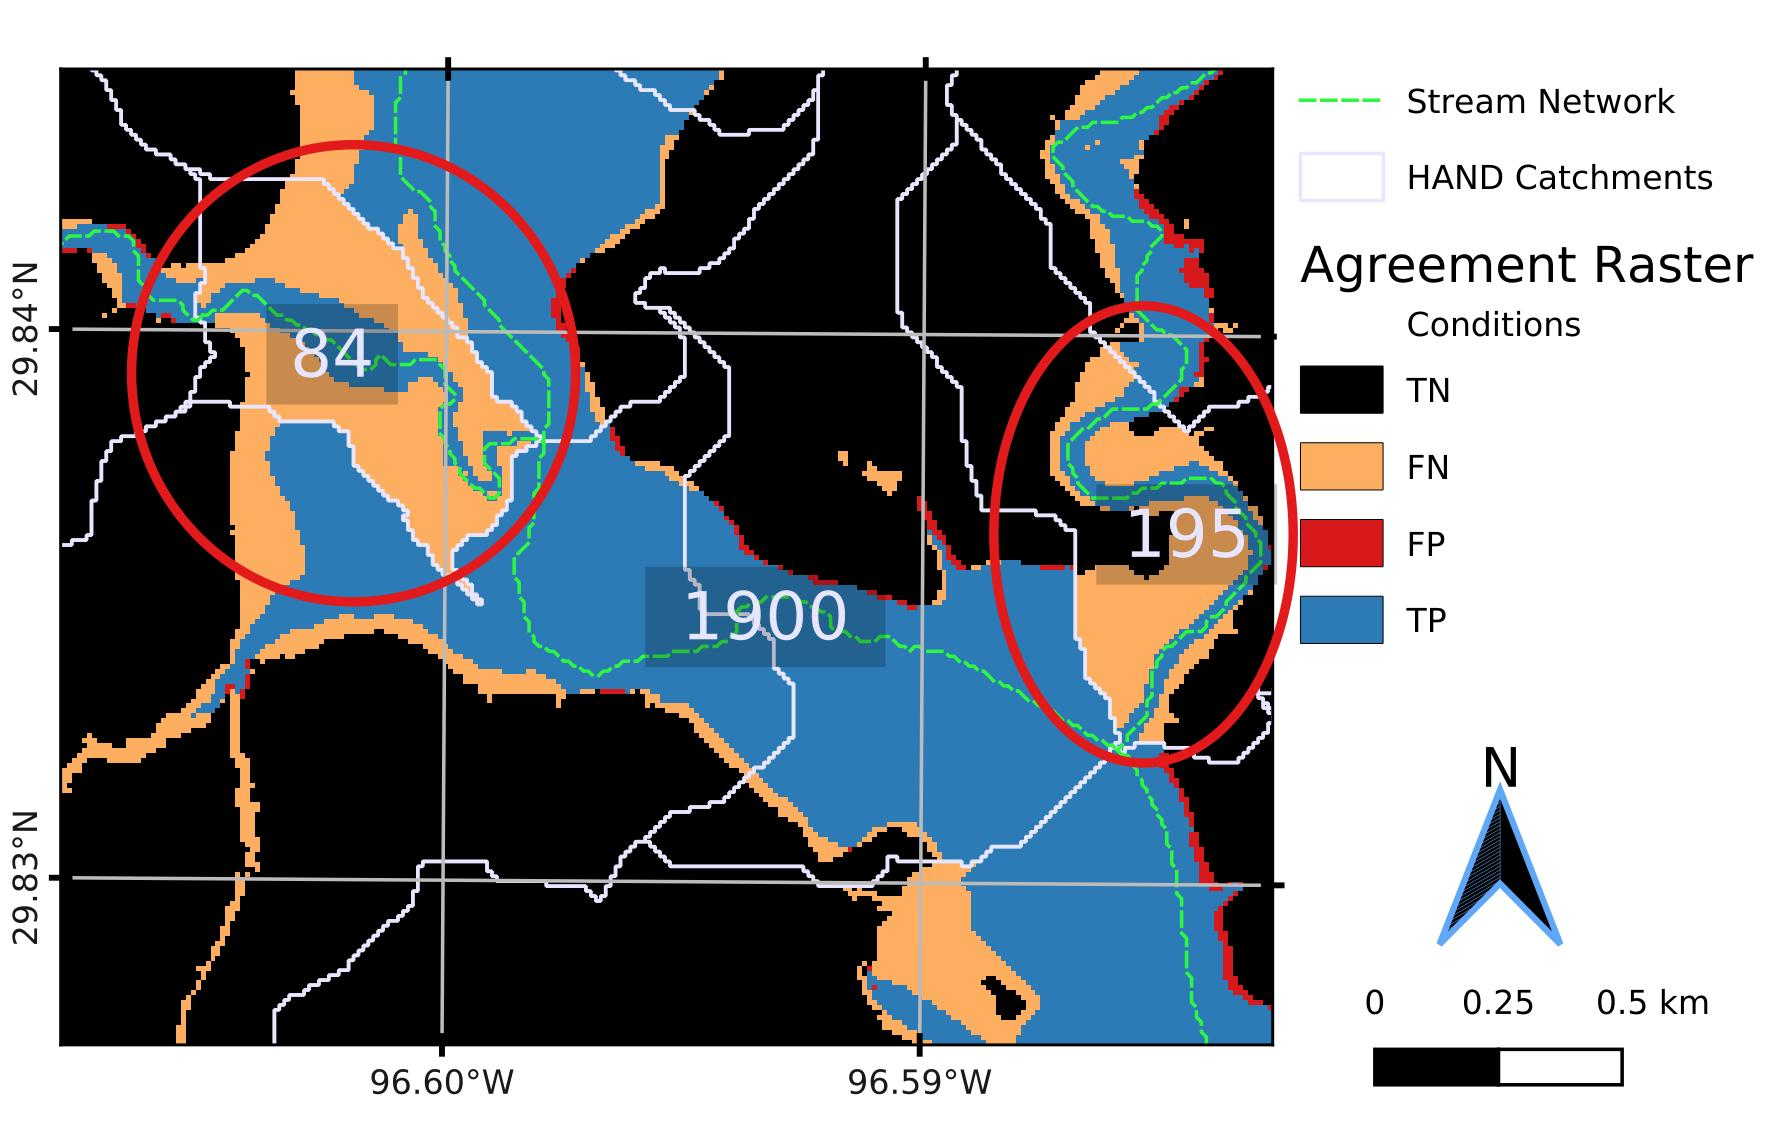
\includegraphics[scale=1.0]{figures/catchment_boundaries_issue.jpg}
\caption{\DIFdelbeginFL \DIFdelFL{False }\DIFdelendFL \DIFaddbeginFL \DIFaddFL{The figure represents an agreement map between a HAND derived FIM and one produced from the Base Level Engineering (BLE) program for a 100 yr magnitude event at HUC8 12090301.
Agreement maps are symbolized by false }\DIFaddendFL negatives \DIFaddbeginFL \DIFaddFL{(FN), true negatives (TN), false positives (FP), and true positives (TP) where inundated represents the positive condition (see Section \ref{ssec:evaluation} for more details).
The streamflows }\DIFaddendFL associated with \DIFaddbeginFL \DIFaddFL{each river segment are shown in CMS while the flow directions are symbolized as red arrows.
The presence of FNs at the }\DIFaddendFL confluence of tributaries \DIFaddbeginFL \DIFaddFL{(circled in red) }\DIFaddendFL with \DIFdelbeginFL \DIFdelFL{MS}\DIFdelendFL \DIFaddbeginFL \DIFaddFL{the main segment is associated with lower flow rates in the tributaries that don't account for backwater effects}\DIFaddendFL .
\DIFdelbeginFL \DIFdelFL{Integers represent }\DIFdelendFL \DIFaddbeginFL \DIFaddFL{Additionally, the }\DIFaddendFL flow \DIFdelbeginFL \DIFdelFL{values }\DIFdelendFL \DIFaddbeginFL \DIFaddFL{of 1900 CMS }\DIFaddendFL from \DIFdelbeginFL \DIFdelFL{BLE 100 year event for }\DIFdelendFL the \DIFdelbeginFL \DIFdelFL{associated areas}\DIFdelendFL \DIFaddbeginFL \DIFaddFL{main segment cannot extend to the neighboring catchments belonging to its tributaries shown here}\DIFaddendFL .
\DIFdelbeginFL \DIFdelFL{No backwater consideration is implemented and }\DIFdelendFL \DIFaddbeginFL \DIFaddFL{Water pools up vertically along }\DIFaddendFL the \DIFdelbeginFL \DIFdelFL{independent nature }\DIFdelendFL \DIFaddbeginFL \DIFaddFL{catchment boundaries }\DIFaddendFL of the \DIFdelbeginFL \DIFdelFL{HAND catchments prohibits pluvial }\DIFdelendFL \DIFaddbeginFL \DIFaddFL{higher order segment distorting rating curve behavior (Section \ref{sec:discussion}).
Sourcing fluvial }\DIFaddendFL inundation from \DIFdelbeginFL \DIFdelFL{taking place}\DIFdelendFL \DIFaddbeginFL \DIFaddFL{HAND is limited to only its nearest drainage line which is the main issue this study aims to address}\DIFaddendFL .
}
\label{fig:catchment_boundaries_issue}
\end{figure}
%
\DIFaddbegin 

\DIFaddend We seek to resolve this \DIFdelbegin \DIFdel{problem by deriving HAND for processing units with stream }\DIFdelend \DIFaddbegin \DIFadd{catchment boundary problem or nearest drainage limitation by discretizing the target stream network into stream }\DIFaddend networks of reduced\DIFdelbegin \DIFdel{stream order. 
}\DIFdelend \DIFaddbegin \DIFadd{, unit stream order to avoid the constraining of catchments by those belonging to lower order neighbors.
By discretizing the network into stream networks of unit stream order (later defined as LP), we remove the influence of neighboring catchments that constrain the inundation extent.
This creates much larger and overlapping catchments that can source fluvial inundation from multiple reaches as required by the given river stage at current flow conditions.
}\DIFaddend We present two successive methods\DIFaddbegin \DIFadd{, National Weather Service MS (Section \ref{sssec:nws_mainstems}) and GMS (Section \ref{sssec:generalized_mainstems}), }\DIFaddend implemented that reduce \DIFdelbegin \DIFdel{drainage densities by reducing }\DIFdelend \DIFaddbegin \DIFadd{the effective }\DIFaddend Horton-Strahler stream orders of the networks employed and test our presented hypothesis that unary stream order networks enhance FIM performance skill with HAND \DIFdelbegin \DIFdel{.
The resulting FIMs from the overlapping HAND processing units are mosaiced together taking any inundated area to be inundated but more will be explained in Section \ref{ssec:inundation_mapping}.
}\DIFdelend \DIFaddbegin \DIFadd{by expanding the nearest drainage definition to increase potential inundation areas.
}

\DIFadd{To clarify the phrase ``reducing Horton-Strahler stream order'' used extensively in this paper, every FIM used in evaluation contains a flood extent sourced from every NWM forecast point in the given evaluation domain.
What we do to reduce stream order is discretize the NWM FR network into different units of size, MS network (\ref{sssec:nws_mainstems}) and GMS LPs (\ref{sssec:generalized_mainstems}), that effectively reduce the HAND computation to independent networks of unit stream order.
These independent HAND datasets are later used to produce FIM independently and mosaiced together (see Section \ref{ssec:inundation_mapping}).
The inundation from the MS HAND is mosaiced with the inundation from FR HAND, while the inundation of each individual LP from GMS is mosaiced together.
The Horton-Strahler stream order is only reduced for HAND computation purposes to reduce the negative effects of the nearest drainage limitation inherent to HAND.
}\DIFaddend %
%%%%%%%%%%%%%%%%%%%%%%%%%%%%%%%%%%%%%%%%%%%%%%%%%%%%%%%%
\subsubsection{NWS \DIFdelbegin \DIFdel{Main-stems}\DIFdelend \DIFaddbegin \DIFadd{Mainstems}\DIFaddend }
\label{sssec:nws_mainstems}
%
The \DIFaddbegin \DIFadd{initial attempt at drainage order reduction to solve the catchment boundary issue was to use a stream network relevant to the NWS forecasting community. 
The }\DIFaddend Mainstems (MS) network is a subset of the NWM \DIFdelbegin \DIFdel{full-resolution (FR ) }\DIFdelend \DIFaddbegin \DIFadd{FR }\DIFaddend network at and downstream of AHPS forecast points as seen in Figure \ref{fig:forecast_points}.
The MS network comprises about 200 thousand km of stream length which is less than 4\% of the FR total stream length of 5.5 million km.
It also spans 121,724 reaches across 1,608 HUC8s.
\DIFdelbegin \DIFdel{HAND was originally derived for this stream network to enhance mapping skill along these critical MS segments \mbox{%DIFAUXCMD
\cite{djokic2019arc}}\hskip0pt%DIFAUXCMD
.
The inundation derived from this stream network is mosaiced with the inundation from the FR network }\DIFdelend \DIFaddbegin \DIFadd{In this technique, we derive HAND using the FR stream network as well as the MS network which was originally proposed by \mbox{%DIFAUXCMD
\citeA{djokic2019arc}}\hskip0pt%DIFAUXCMD
.
Inundation is derived independently from the resulting FR and MS HAND hydrofabrics and are mosaiced together using the technique proposed in Section \ref{ssec:inundation_mapping} }\DIFaddend to form the MS FIMs. 
Within each HUC, \DIFdelbegin \DIFdel{you'll }\DIFdelend \DIFaddbegin \DIFadd{one might }\DIFaddend typically only find a MS stream network of \DIFdelbegin \DIFdel{stream order 1 (i.e. headwater) }\DIFdelend \DIFaddbegin \DIFadd{uniform stream order }\DIFaddend but this can vary if more than one AHPS forecasting point is found within or upstream of the HUC in question.
\DIFaddbegin \DIFadd{So while we may refer to the MS network as that of one with unit stream order, we acknowledge there are many cases where additional or converging forecast points create multiple branches within a given processing unit.
}\DIFaddend %
%%%%%%%%%%%%%%%%%%%%%%%%%%%%%%%%%%%%%%%%%%%%%%%%%%%%%%%%
\subsubsection{Generalized Mainstems}
\label{sssec:generalized_mainstems}
%DIF < 
\DIFdelbegin \DIFdel{To further the efforts implemented by MS }\DIFdelend %DIF > 
\DIFaddbegin \DIFadd{Since MS only covers 4\% of the entire FR stream network}\DIFaddend , we \DIFdelbegin \DIFdel{sought to derive HAND at a level path scale which we call GMS.
Since the MS network only covers a small percentage of the NWM forecasting domain, we }\DIFdelend sought to expand \DIFdelbegin \DIFdel{the benefits of stream order reduction within HAND processing units to the entire FR domain.
Level paths }\DIFdelend \DIFaddbegin \DIFadd{drainage order reduction techniques to all reaches within the NWM modeling domain.
In order to do this, we discretized the NWM network into LPs which when considered individually have unit Horton-Strahler stream orders.
LPs }\DIFaddend group flowlines by maximizing the length of each flow path and minimizing the number of \DIFdelbegin \DIFdel{level path }\DIFdelend \DIFaddbegin \DIFadd{LP }\DIFaddend identifiers within a given domain \cite{moore2019user,mckay2012nhdplus}. 
\DIFdelbegin \DIFdel{Starting at the }\DIFdelend \DIFaddbegin \DIFadd{In order to derive LPs for the NWM FR stream network at the HUC8 processing area, we first compute arbolate sums which are defined as the cumulative drainage distance of all upstream drainage lines.
Arbolate sum is also inclusive of the current drainage reach as well.
Arbolate sums are computed by starting at the headwater points and summing up drainage distances as you traverse downstream.
}

\DIFadd{Arbolate sum is critical to discretizing the NWM network into LP identifiers.
Starting at a HUC8's }\DIFaddend outlet, a unique \DIFdelbegin \DIFdel{level path }\DIFdelend \DIFaddbegin \DIFadd{LP }\DIFaddend is propagated upstream. 
At every confluence, the direction of maximum \DIFdelbegin \DIFdel{flow path length }\DIFdelend \DIFaddbegin \DIFadd{arbolate sum }\DIFaddend is sought to propagate the current \DIFdelbegin \DIFdel{level path }\DIFdelend \DIFaddbegin \DIFadd{LP }\DIFaddend identifier.
For the remaining parent reaches of the given junction, a new \DIFdelbegin \DIFdel{level path }\DIFdelend \DIFaddbegin \DIFadd{LP }\DIFaddend identifier is assigned and the process recursively continues with them.
Figure \ref{fig:level_path_methods} \DIFdelbegin \DIFdel{illustrate how level paths }\DIFdelend \DIFaddbegin \DIFadd{illustrates how LPs }\DIFaddend (symbolized by unique colors) are propagated upstream by the value of arbolate sum.
\DIFaddbegin \DIFadd{The figure shows computed arbolate sums and unique LP identifiers on a HUC12 (120903010404) for clarity but were computed at the corresponding HUC8.
The mainstem of the figure runs from the red ellipses to the black one which is the outlet.
From the figure, we can see how unique colors are propagated in the direction of the maximum arbolate sum.
}

\DIFaddend Each HUC8 is discretized into \DIFdelbegin \DIFdel{level paths independently and relevant inputs }\DIFdelend \DIFaddbegin \DIFadd{LPs independently and the relevant inputs as described in Table \ref{tab:data} }\DIFaddend are assigned to each \DIFdelbegin \DIFdel{level path }\DIFdelend \DIFaddbegin \DIFadd{LP }\DIFaddend processing unit given a buffer of \DIFdelbegin \DIFdel{7 km.
At the level path }\DIFdelend \DIFaddbegin \DIFadd{seven km.
This buffer was selected to avoid edge contamination \mbox{%DIFAUXCMD
\cite{lindsay2013measuring} }\hskip0pt%DIFAUXCMD
and to ensure adequate data availability for wide rivers with large catchments in regions with low slope.
Further work could be dedicated to tune this user exposed parameter to better balance its effect on FIM extents and computational expense since larger buffers create additional floating point calculations and storage requirements.
For the time being, we designate this issue to be out of scope.
}

\DIFadd{At the LP }\DIFaddend scale, the methods in Sections \ref{ssec:hydro_conditioning} and \ref{ssec:deriving_fim_hydrofabric} are executed leaving out any tributaries of the \DIFdelbegin \DIFdel{level path }\DIFdelend \DIFaddbegin \DIFadd{LP }\DIFaddend in question at the time.
The only exception to this is the use of the NWM stream network directly for use with hydro-enforcement \DIFdelbegin \DIFdel{which }\DIFdelend \DIFaddbegin \DIFadd{by burning these lines and seeding from its headwater points directly instead of going through the NHDPlusHR network as described in Section \ref{ssec:stream_network_enforcment} .
This decision }\DIFaddend was motivated by the difficulty in deriving \DIFdelbegin \DIFdel{level paths }\DIFdelend \DIFaddbegin \DIFadd{LPs }\DIFaddend in the NWM stream network with high agreement with the \DIFaddbegin \DIFadd{LPs derived for the }\DIFaddend NHDPlusHR stream lines.
\DIFaddbegin \DIFadd{We found that the same algorithm to compute arbolate sums and LPs could yield enough disagreements associated with disordered branches or slight differences in arbolate sums that could significantly affect the agreement of the LP identifiers in the NWM and NHDPlusHR networks.
This yielded enough error to justify the use of the NWM directly for hydro-enforcement operations.
}\DIFaddend 

\DIFaddbegin \DIFadd{Once the NWM FR stream network is discretized into LPs, we independently compute HAND using each LP as the target stream network to be used.
}\DIFaddend To illustrate the GMS procedure, we reference Figure \ref{fig:gms_methods} to show how deriving HAND and FIMs from GMS works.
In Figure \ref{fig:gms_methods}a, we uniquely color code the \DIFdelbegin \DIFdel{level paths }\DIFdelend \DIFaddbegin \DIFadd{LPs }\DIFaddend derived for the NWM stream network. 
For each one of these lines, we derive HAND and its associated datasets including catchments, crosswalks, and rating curves.
Each \DIFdelbegin \DIFdel{level path }\DIFdelend \DIFaddbegin \DIFadd{LP }\DIFaddend is buffered to a polygon with a \DIFdelbegin \DIFdel{user-available }\DIFdelend \DIFaddbegin \DIFadd{user-exposed, }\DIFaddend distance parameter of \DIFdelbegin \DIFdel{7 km and this polygon }\DIFdelend \DIFaddbegin \DIFadd{seven km that }\DIFaddend is used to subset the original DEM for two selected \DIFdelbegin \DIFdel{level paths }\DIFdelend \DIFaddbegin \DIFadd{LPs }\DIFaddend in Figure \ref{fig:gms_methods}b.
We illustrate two HAND grids for two of the \DIFdelbegin \DIFdel{level paths }\DIFdelend \DIFaddbegin \DIFadd{LPs }\DIFaddend in this HUC8 in Figure \ref{fig:gms_methods}c.
Once the FIM hydrofabrics for each \DIFdelbegin \DIFdel{level path }\DIFdelend \DIFaddbegin \DIFadd{LP }\DIFaddend are generated, we can inundate them individually also shown in Figure \ref{fig:gms_methods}d.
Lastly\DIFaddbegin \DIFadd{, }\DIFaddend these individual FIMs are mosaiced together as explained in Section \ref{ssec:inundation_mapping} and shown in Figure \ref{fig:gms_methods}\DIFdelbegin \DIFdel{c.
}\DIFdelend \DIFaddbegin \DIFadd{d.
}

\DIFadd{For a more intimate look at the drainage order reduction procedure GMS, and its effects, we allude to Figure \ref{fig:gms_methods_2} which references the same area (in HUC8 12090301) and set of river junctions as in Figure \ref{fig:catchment_boundaries_issue}.
The catchments and stream lines for HAND computed at the FR scale are illustrated in Figure \ref{fig:gms_methods_2}a where the respective inundation at the 100 yr magnitude is heavily constrained by the limited catchment extents especially at junctions.
In subsequent sub-figures, we show the same datasets for the HAND computation problem for this region but discretized into independent LPs for the main LP (b), the eastern tributary (c), and the western tributary (d).
Notably, inspecting (b), one sees how removing the tributaries creates much larger catchments for the main LP. 
These catchments include drainage areas that would traditionally be considered nearest to the tributaries thus ineligible to receive inundation sourced from the main LP.
The inundation extents in (b) overlap those of (c) and (d) and are mosaiced together by methods explained in Section \ref{ssec:inundation_mapping}.
}\DIFaddend %
\DIFdelbegin %DIFDELCMD < \begin{figure}[h!]
%DIFDELCMD < %%%
\DIFdelendFL \DIFaddbeginFL \begin{figure}[H]
\DIFaddendFL \centering
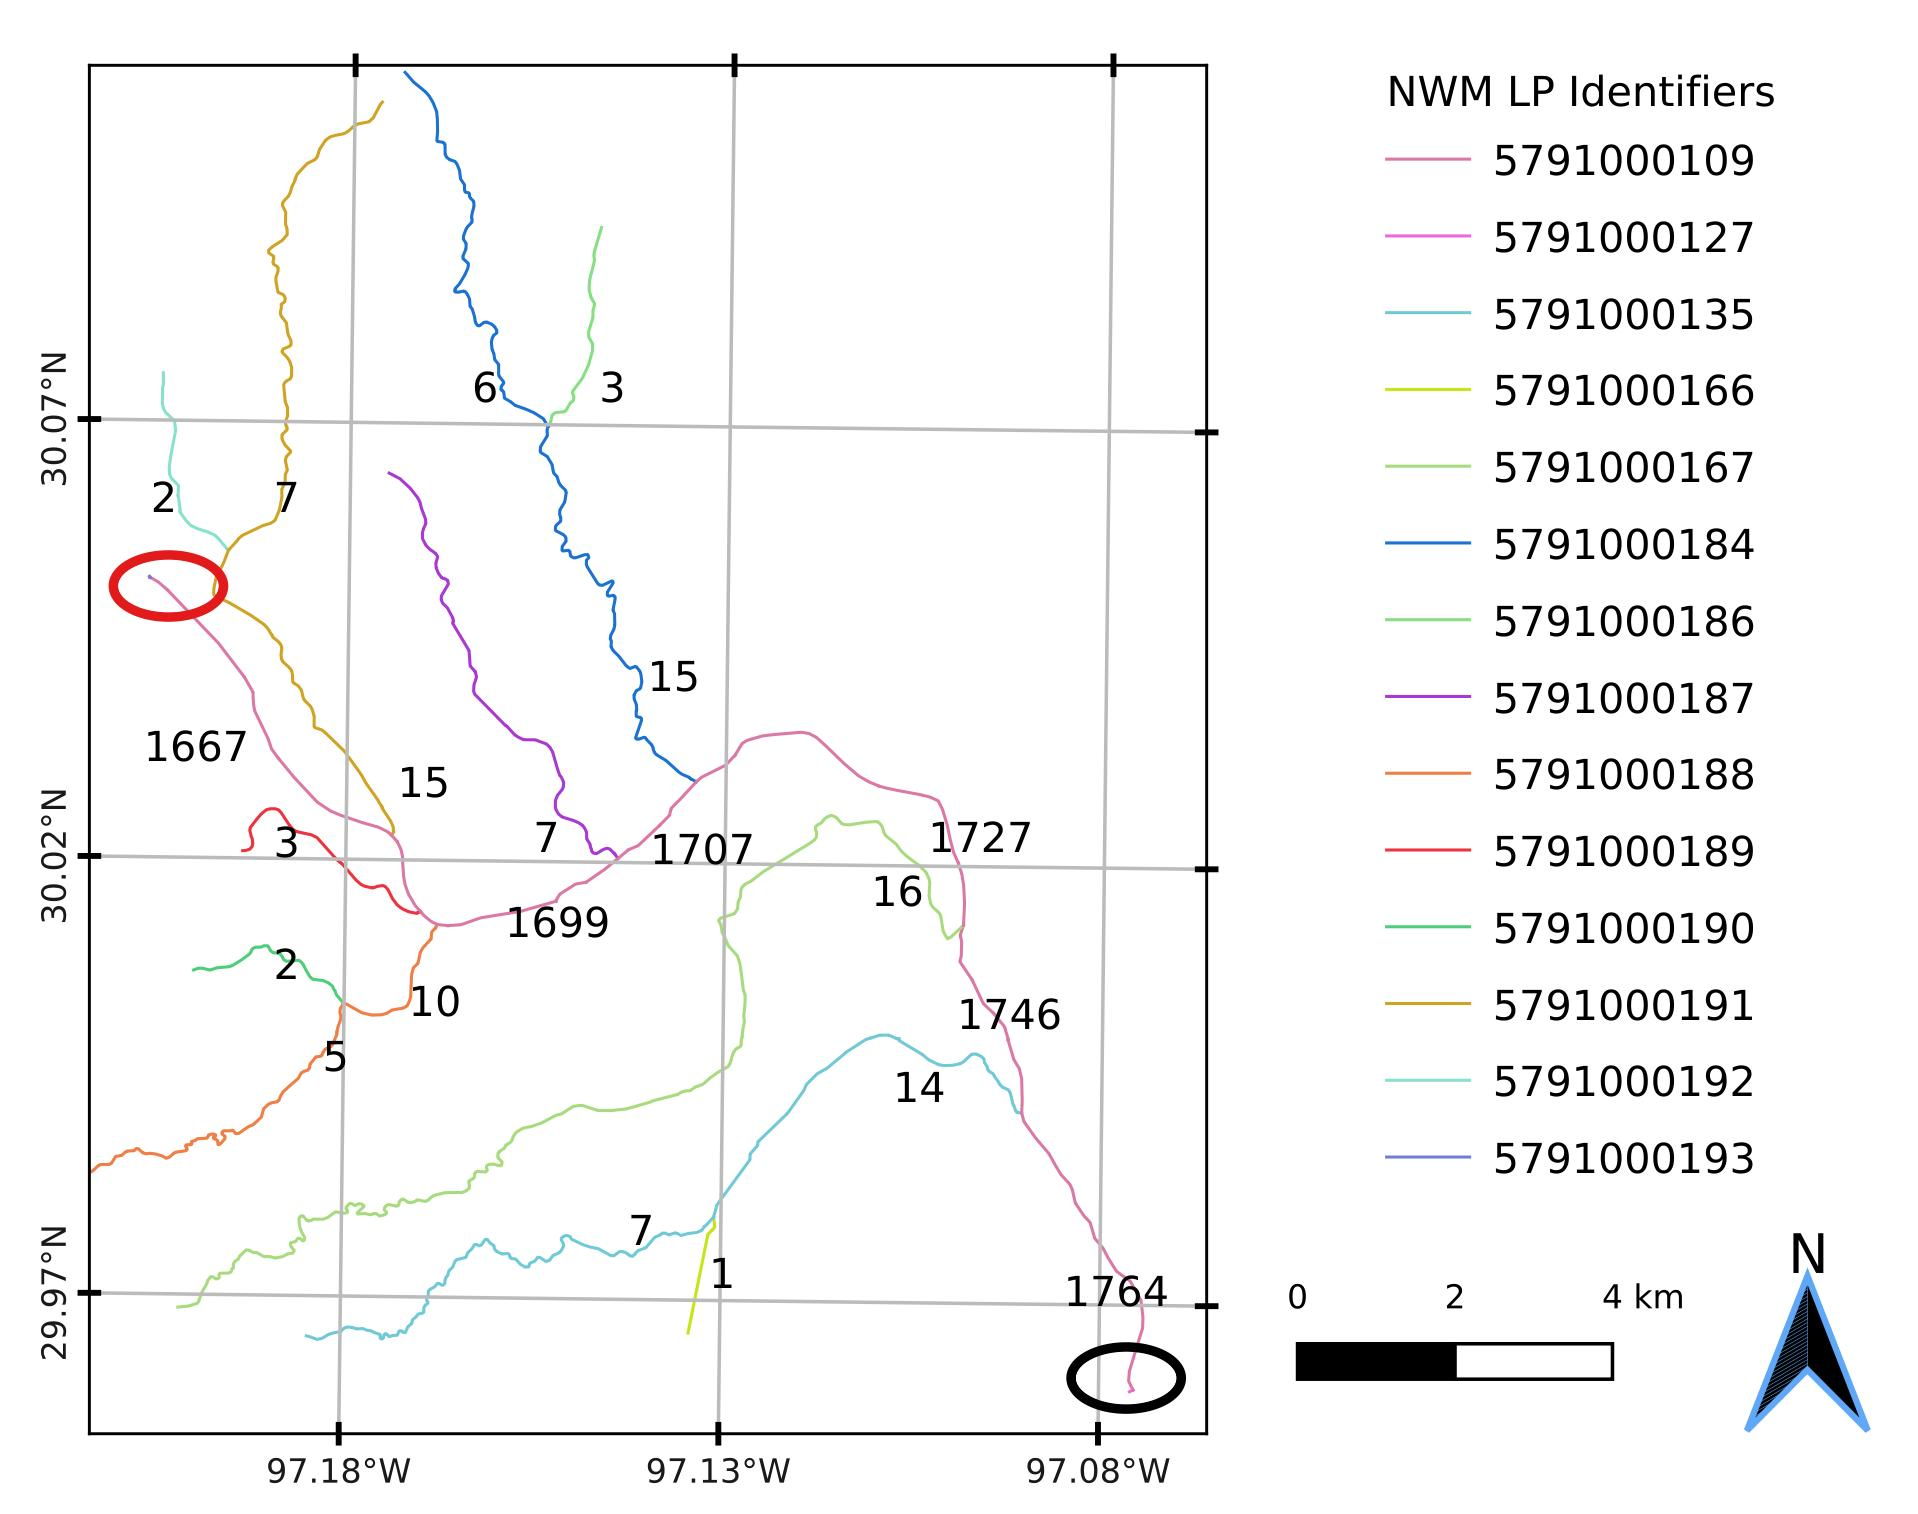
\includegraphics[scale=1.0]{figures/level_path_methods.jpg}
\caption{Illustrates \DIFdelbeginFL \DIFdelFL{how }\DIFdelendFL \DIFaddbeginFL \DIFaddFL{the NWM Full Resolution V2.1 stream network discretized into }\DIFaddendFL level paths \DIFaddbeginFL \DIFaddFL{(LP), symbolized by unique colors, as well as the values of the arbolate sums to the nearest whole km distance.
The LPs were derived on a HUC8 level (12090301) but only illustrated }\DIFaddendFL for \DIFaddbeginFL \DIFaddFL{a HUC12 (120903010404) for clarity.
The mainstem of this HUC12 runs from }\DIFaddendFL the \DIFaddbeginFL \DIFaddFL{red ellipses to the outlet denoted by the black ellipses.
Arbolate sums are defined as the cumulative drainage distances of all upstream stream lines.
Arbolate sums are computed for the }\DIFaddendFL NWM \DIFaddbeginFL \DIFaddFL{network by starting at the headwater points then traversing downstream and adding the distances cumulatively. 
LPs }\DIFaddendFL are derived \DIFdelbeginFL \DIFdelFL{.
Level paths symbolized }\DIFdelendFL by \DIFdelbeginFL \DIFdelFL{lines of }\DIFdelendFL \DIFaddbeginFL \DIFaddFL{starting at an outlet point with a }\DIFaddendFL unique \DIFdelbeginFL \DIFdelFL{colors are }\DIFdelendFL \DIFaddbeginFL \DIFaddFL{identifier (ID).
The unique LP ID is }\DIFaddendFL propagated upstream \DIFdelbeginFL \DIFdelFL{following }\DIFdelendFL \DIFaddbeginFL \DIFaddFL{until a junction is reached where }\DIFaddendFL the \DIFaddbeginFL \DIFaddFL{current LP ID is propagated in the }\DIFaddendFL direction of maximum arbolate sum\DIFaddbeginFL \DIFaddFL{.
The remaining converging segments }\DIFaddendFL at \DIFdelbeginFL \DIFdelFL{each }\DIFdelendFL \DIFaddbeginFL \DIFaddFL{the given }\DIFaddendFL junction \DIFaddbeginFL \DIFaddFL{are each assigned a new unique LP ID and the process is repeated recursively until all reaches have been assigned a LP}\DIFaddendFL .
\DIFaddbeginFL \DIFaddFL{Thus, LP serve as a proxy means of assigning membership to a given river when presented with a confluence.
Each individual LP has a unit Horton-Strahler stream order thus serves as a great method for our proposed technique.
}\DIFaddendFL }
\label{fig:level_path_methods}
\end{figure}
%
%
\DIFdelbegin %DIFDELCMD < \begin{figure}[h!]
%DIFDELCMD < %%%
\DIFdelendFL \DIFaddbeginFL \begin{figure}[H]
\DIFaddendFL \centering
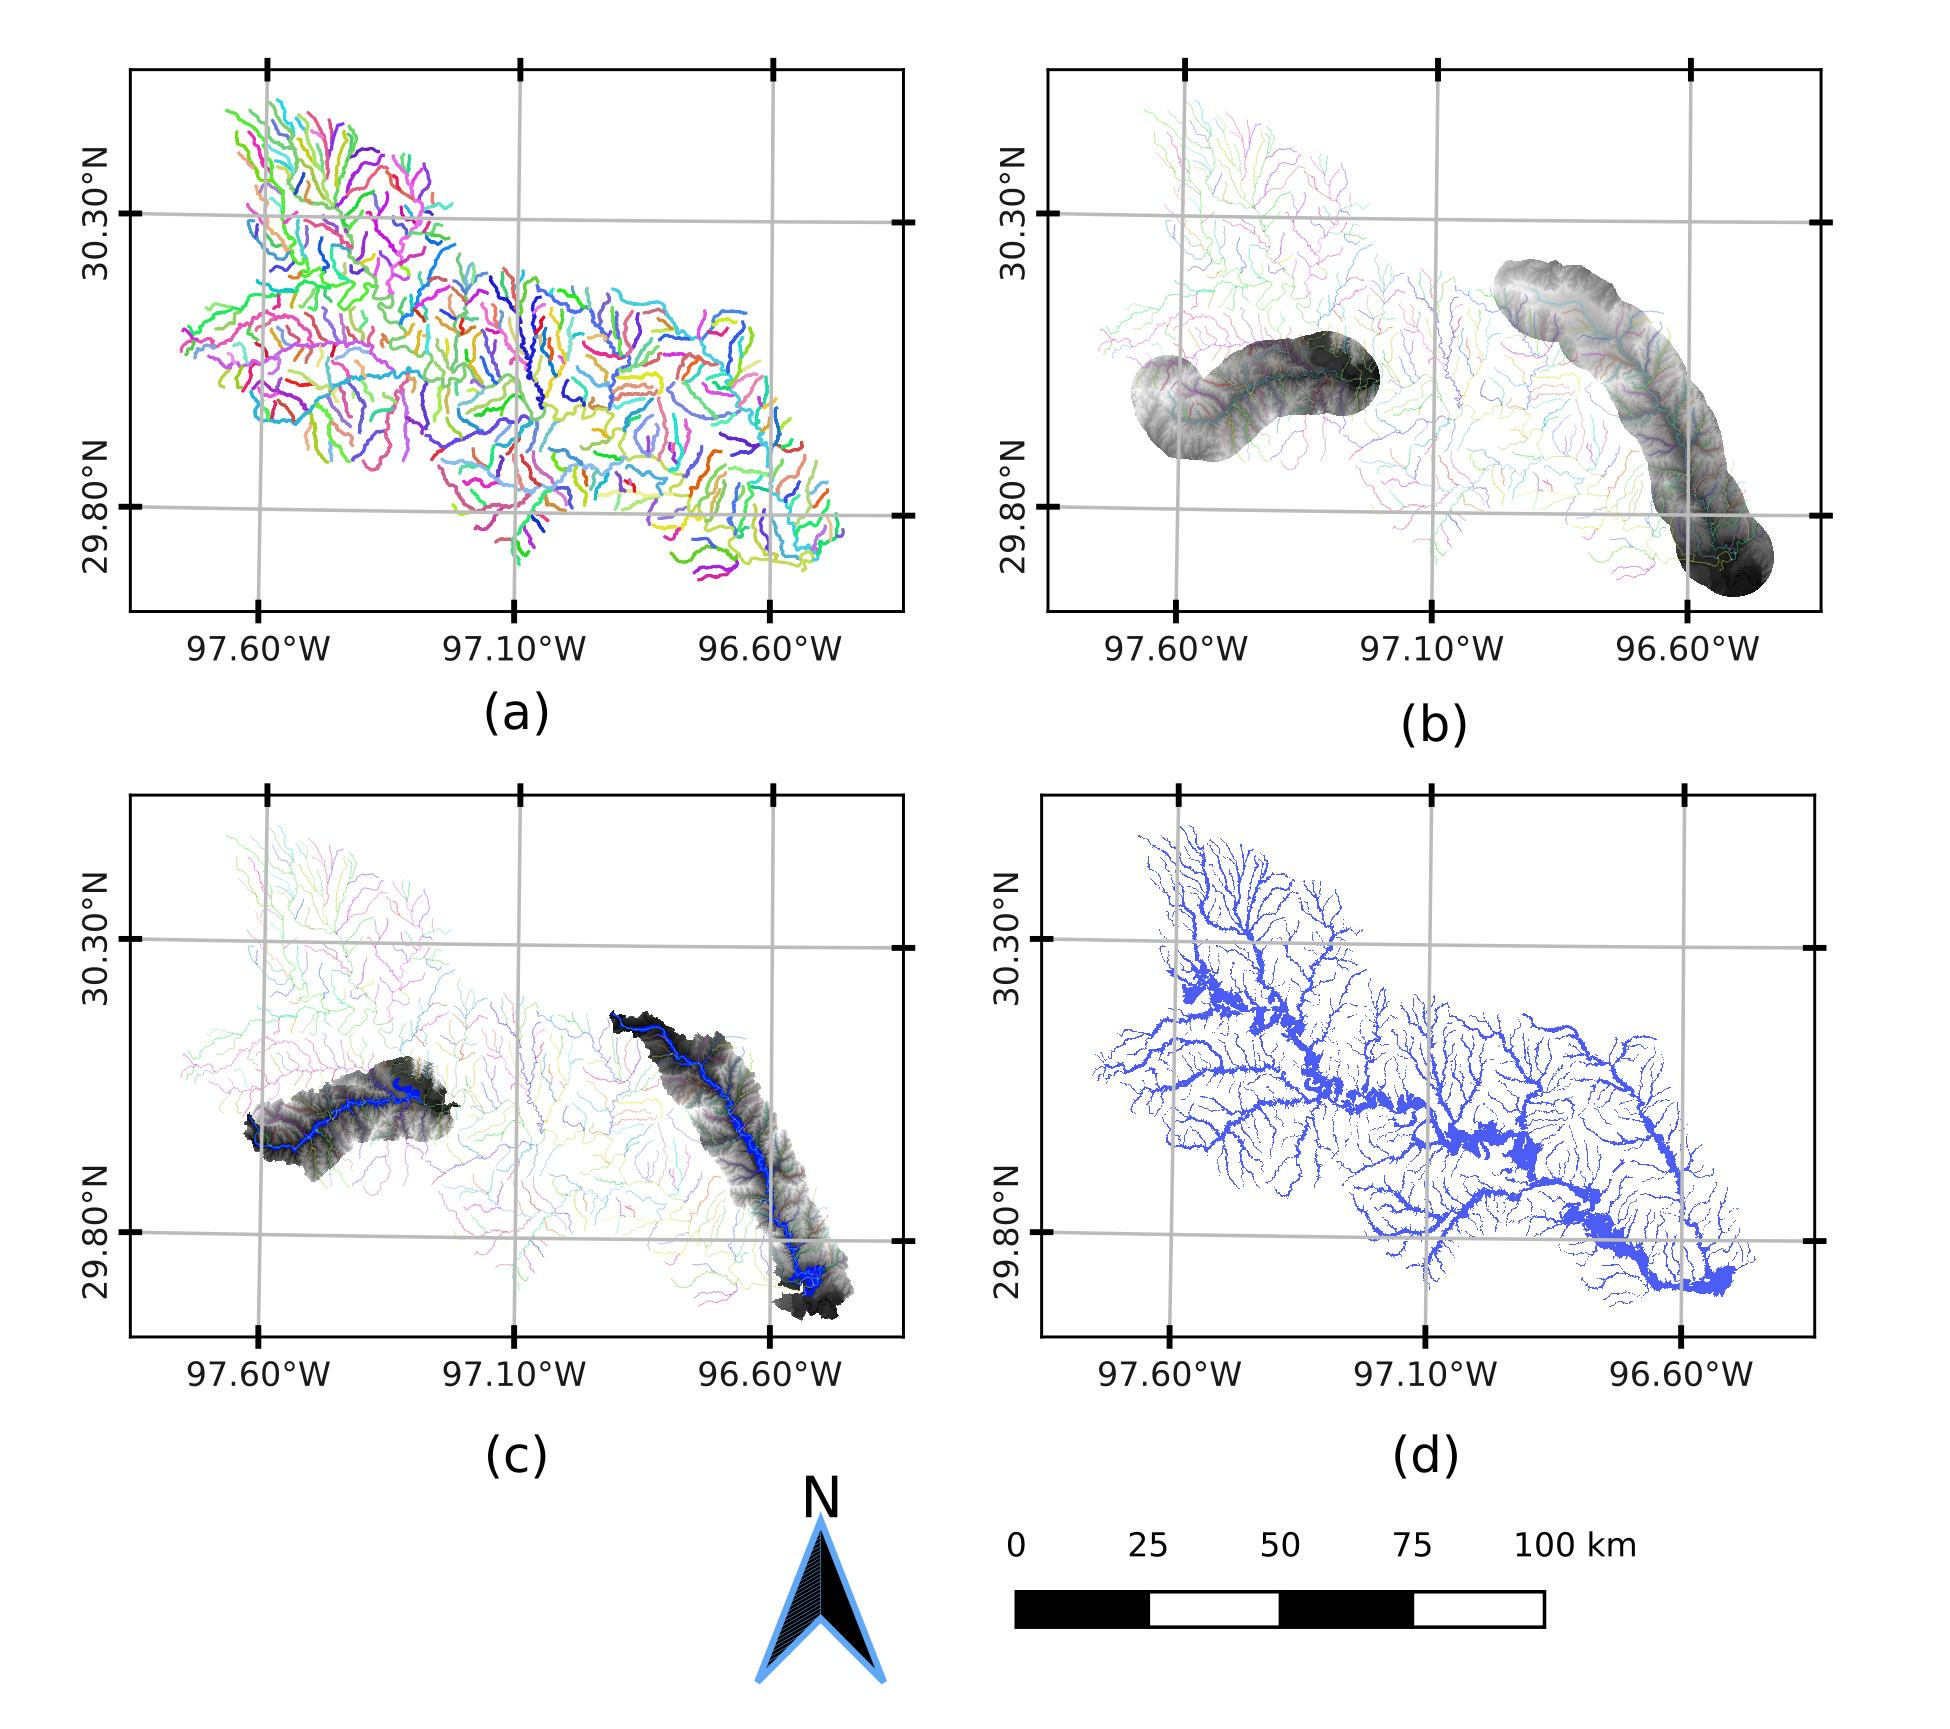
\includegraphics[scale=1.0]{figures/gms_methods.jpg}
\caption{Overall procedure for GMS HAND \DIFdelbeginFL \DIFdelFL{.
}\DIFdelendFL \DIFaddbeginFL \DIFaddFL{at HUC8 12090301.
}\DIFaddendFL In (a), we illustrate all NWM stream lines symbolized by their \DIFdelbeginFL \DIFdelFL{level path}\DIFdelendFL \DIFaddbeginFL \DIFaddFL{LP with 372 unique LP IDs in this HUC}\DIFaddendFL .
Meanwhile (b), demonstrates the DEM clipped to a \DIFdelbeginFL \DIFdelFL{7 }\DIFdelendFL \DIFaddbeginFL \DIFaddFL{seven }\DIFaddendFL km buffer around two selected \DIFdelbeginFL \DIFdelFL{level paths}\DIFdelendFL \DIFaddbeginFL \DIFaddFL{LPs}\DIFaddendFL .
In (c), we show how HAND can be computed just for each one of these two \DIFdelbeginFL \DIFdelFL{level paths }\DIFdelendFL \DIFaddbeginFL \DIFaddFL{LPs }\DIFaddendFL independently. 
We also show inundation maps created for these two \DIFdelbeginFL \DIFdelFL{level paths }\DIFdelendFL \DIFaddbeginFL \DIFaddFL{LPs }\DIFaddendFL in (c). 
In (d), we show all the inundation maps for all the \DIFdelbeginFL \DIFdelFL{level paths }\DIFdelendFL \DIFaddbeginFL \DIFaddFL{LPs }\DIFaddendFL mosaiced together. }
\label{fig:gms_methods}
\end{figure}
%
%DIF > 
\DIFaddbegin \begin{figure}[H]
\centering
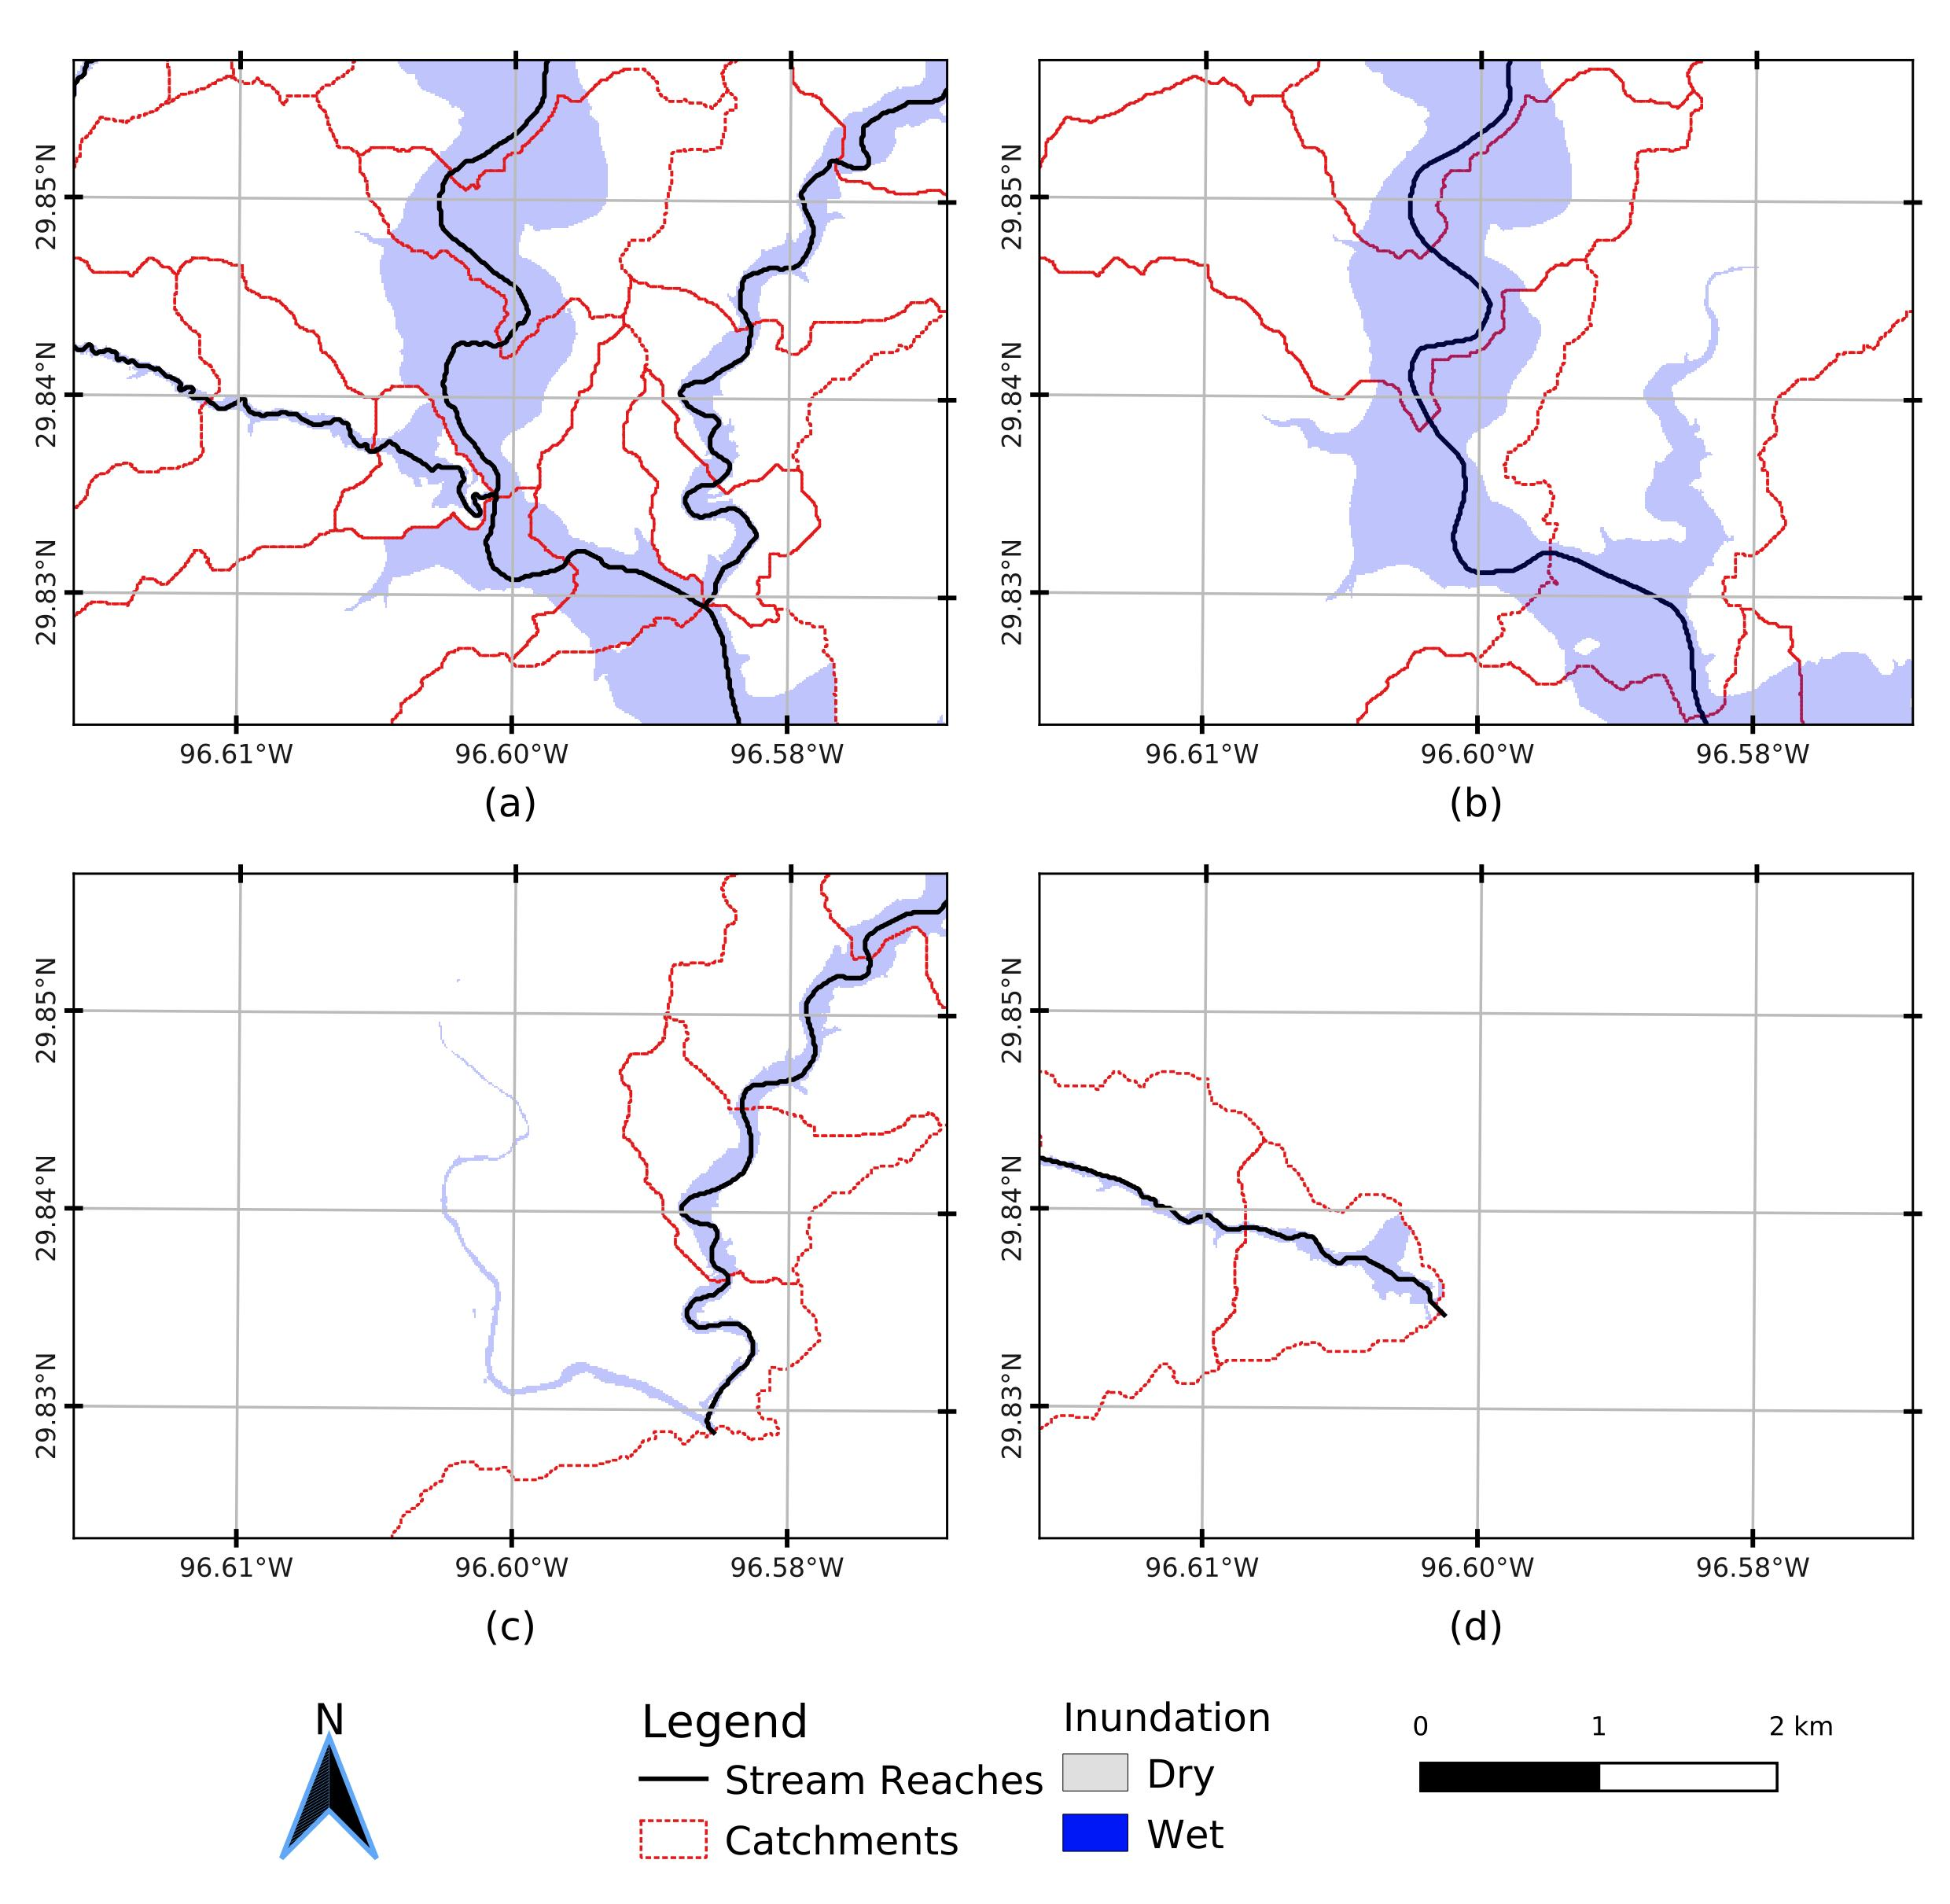
\includegraphics[scale=0.70]{figures/gms_methods_2.jpg}
\caption{\DIFaddFL{This image, with the same spatial domain as Figure \ref{fig:catchment_boundaries_issue} (HUC 12090301), demonstrates how computing HAND on level path (LP) bases leads to larger, independent catchments and more expansive inundation extents (100 yr flows).
In (a), the catchments and stream network are shown for HAND computed in Full-Resolution (FR) method which shows constrained inundation extents around the two junctions.
(b) demonstrates the LP associated with this region's highest order river.
By delineating catchments at this scale independent of the neighboring tributaries, the drainage areas are allowed to expand thus allowing inundation extents to cover previously restricted areas.
In (c) and (d), we show the stream lines, catchments, and inundation extents of the two tributaries.
Later in Section \ref{ssec:inundation_mapping}, we describe how the inundation in (b), (c), and (d) are mosaiced together to form one seamless inundation map.
This process allows for multiple, possible contributing sources of fluvial inundation to be considered thus enhancing FIM skill.
}}
\label{fig:gms_methods_2}
\end{figure}
%DIF > 
\DIFaddend %%%%%%%%%%%%%%%%%%%%%%%%%%%%%%%%%%%%%%%%%%%%%%%%%%%%%%%%
\subsection{Inundation Mapping}
\label{ssec:inundation_mapping}
%
The FIM hydrofabric consisting of the relative elevations grid, catchments grid, catchment polygons, rating curve, and cross-walking data are all used to convert forecasts from the NWM into forecasts extents.
For operational situations, one would cache the FIM hydrofabric then either produce libraries of FIM for a sample of discharges or stages or also produce the FIM in near real-time (NRT).
From the cached FIM hydrofabric and design or forecast discharges including those extracted from the NWM, inundation maps can be generated at \DIFdelbegin \DIFdel{HUC 8 }\DIFdelend \DIFaddbegin \DIFadd{HUC8 }\DIFaddend spatial processing units in a rapid, parallel operation. 
The discharges are associated with NWM reach identifiers and cross-walked over to reach identifiers in the FIM hydrofabric.


Utilizing the stage-discharge relationships in the \DIFdelbegin \DIFdel{synthetic rating curves}\DIFdelend \DIFaddbegin \DIFadd{SRCs}\DIFaddend , each forecast for each catchment identifier is assigned a stage value. 
The catchments grid encoded with the reach identifiers are used to map the stages by thresholding to the forecast stage.
We use the basic logic already established in previous works to conduct this \cite{nobre2016hand,liu2016cybergis,maidment2017conceptual}.
Mathematically, the HAND values, $H_{ij}$, can be indexed by the reach identifiers, i, and pixel indices, j.
For each forecast stage, $S_i$, one can express the formula for $D_{ij}$, a continuous variable denoting water depth at a given pixel with reach and pixel identifiers i and j respectively in Equation \ref{eq:hand_fim_depth}.
For each forecast stage, $S_i$, one can express the formula for $F_{ij}$, a binary variable denoting inundation condition in Equation \ref{eq:hand_fim} in terms of $D_{ij}$ by simply thresholding at zero depths.
%
\begin{linenomath*}
\begin{equation}
\label{eq:hand_fim_depth}
    D_{ij} = S_i - H_{ij}
\end{equation}
\end{linenomath*}
%
\begin{linenomath*}
\begin{equation}
\label{eq:hand_fim}
    F_{ij} = D_{ij} > 0
\end{equation}
\end{linenomath*}
%
For the cases of MS and GMS, the inundation maps produced for the respective processing units at lower maximum stream orders must be mosaiced together to form a seamless forecast in the form of a single raster file.
For mosaicing the depths, we select the maximum inundation depth from the all the contributing areas K index by its lower case character, k.
\DIFaddbegin \DIFadd{Consolidating the depths using a maximum function was decided upon based on intuition which we believe to best represent the depth of water in an area with multiple contributing fluvial inundation sources.
Other aggregation methods could lead to different results but were not investigated here.
}\DIFaddend Equation \ref{eq:comp_fim_depths} illustrates how the maximum depth from all the contributing areas, k, to each pixel j in catchment i\DIFaddbegin \DIFadd{,
%DIF > 
}\begin{linenomath*}
\begin{equation}
\DIFadd{\label{eq:comp_fim_depths}
    D_{ij} = \max_{k=[1,...,K]} D_{ijk}
}\end{equation}
\end{linenomath*}
%DIF > 
\DIFaddend . Equation \ref{eq:comp_fim} illustrates the same process but for mosaicing the binary inundation maps\DIFdelbegin \DIFdel{.
}\DIFdelend \DIFaddbegin \DIFadd{,
}\DIFaddend %
\begin{linenomath*}
\begin{equation}
\DIFdelbegin %DIFDELCMD < \label{eq:comp_fim_depths}
%DIFDELCMD <     %%%
\DIFdel{D}\DIFdelend \DIFaddbegin \label{eq:comp_fim}
    \DIFadd{F}\DIFaddend _{ij} = \max_{k=[1,...,K]} \DIFdelbegin \DIFdel{D}\DIFdelend \DIFaddbegin \DIFadd{F}\DIFaddend _{ijk}
\end{equation}
\end{linenomath*}
%DIF < 
\DIFaddbegin \DIFadd{. }\DIFaddend For the MS and GMS methods, the contributing areas are defined differently.
For MS, the FIM from MS HAND and FR HAND are mosaiced together to form a singular inundation map thus K is set to \DIFdelbegin \DIFdel{2 }\DIFdelend \DIFaddbegin \DIFadd{two }\DIFaddend for that case.
For GMS, all FIMs from all the \DIFdelbegin \DIFdel{level paths }\DIFdelend \DIFaddbegin \DIFadd{LPs }\DIFaddend in a given area are mosaiced together then K is set to this number of \DIFdelbegin \DIFdel{level paths}\DIFdelend \DIFaddbegin \DIFadd{LPs}\DIFaddend .
Figures \ref{fig:gms_methods}a and \ref{fig:gms_methods}b, illustrate how inundation maps are created for lower stream order processing units then mosaiced together.
%
\DIFdelbegin %DIFDELCMD < \begin{linenomath*}
%DIFDELCMD < %%%
\begin{displaymath}
\DIFdel{\label{eq:comp_fim}
    F_{ij} = \max_{k=[1,...,K]} F_{ijk}
}\end{displaymath}%DIFAUXCMD
%DIFDELCMD < \end{linenomath*}
%DIFDELCMD < %%%
%DIF < 
\DIFdelend %%%%%%%%%%%%%%%%%%%%%%%%%%%%%%%%%%%%%%%%%%%%%%%%%%%%%%%%
\subsection{Evaluation}
\label{ssec:evaluation}
%%%%%%%%%%%%%%%%%%%%%%%%%%%%%%%%%%%%%%%%%%%%%%%%%%%%%%%%
%
\DIFaddbegin \DIFadd{Possible benchmark FIM candidates for evaluation purposes include high water marks, remote sensing observation, crowd-sourced information, and modeled extents.
These sources are all subject to limitations for evaluating a continental scale model like OWP FIM such as but not limited to a lack of spatial coverage, signal interference, lack of streamflow data, inaccurate streamflow data, physics-based assumptions, and errors in input data.
While in-situ observations such as high water marks offer the highest accuracy, they are often limited in spatial extent and can lack the associated streamflow data necessary to make FIMs to compare to as to isolate out other hydrological factors.
}

\DIFaddend Evaluation of our relative elevation CFIM method is conducted by comparison to the HEC-RAS 1D \DIFdelbegin \DIFdel{derived }\DIFdelend models produced within FEMA region 6 \DIFdelbegin \DIFdel{\mbox{%DIFAUXCMD
\cite{fema2021base,fema2021estimated}}\hskip0pt%DIFAUXCMD
.
}\DIFdelend \DIFaddbegin \DIFadd{\mbox{%DIFAUXCMD
\cite{fema2021base,fema2021estimated,us2022hydrologic}}\hskip0pt%DIFAUXCMD
.
This dataset was selected due to its large spatial coverage, availability of cross-sections with streamflow information, higher level of sophistication when compared to HAND, engineering scale detail, and a storied use in the literature as an evaluation dataset \mbox{%DIFAUXCMD
\cite{cook2009effect,rajib2016large,zheng2018geoflood,afshari2018comparison,wing2017validation,criss2022stage,follum2017autorapid}}\hskip0pt%DIFAUXCMD
.
We selected }\DIFaddend 49 \DIFdelbegin \DIFdel{HUC 8's spanning }\DIFdelend \DIFaddbegin \DIFadd{available HUC8s, shown in Figure \ref{fig:all_ble_maps}, which span }\DIFaddend about 185 thousand \DIFdelbegin \DIFdel{square km were available at the time (now more) }\DIFdelend \DIFaddbegin \DIFadd{$km^2$ }\DIFaddend across nine states\DIFdelbegin \DIFdel{and shown in Figure \ref{fig:all_ble_maps}}\DIFdelend .
The maps \DIFdelbegin \DIFdel{to }\DIFdelend \DIFaddbegin \DIFadd{of }\DIFaddend the 1\% recurrence flow (1 in 100 year) and the 0.2\% recurrence flow (1 in 500 year) are furnished by InFRM \DIFdelbegin \DIFdel{so we used those }\DIFdelend \DIFaddbegin \DIFadd{as well as the }\DIFaddend corresponding discharges and mapping extents for evaluation.
We did exclude NWM V2.1 Reservoirs from evaluation because these are not properly accounted for in the inundation \DIFdelbegin \DIFdel{.
}\DIFdelend \DIFaddbegin \DIFadd{sourced from OWP FIM.
}

\DIFaddend By using the same HEC-RAS derived discharges and FIM extents \DIFaddbegin \DIFadd{for creating maps with OWP FIM}\DIFaddend , we are able to separate out errors introduced by \DIFdelbegin \DIFdel{hydrology, }\DIFdelend \DIFaddbegin \DIFadd{NWM inputs and processes including land surface interactions, groundwater fluxes, }\DIFaddend atmospheric forcings, hydraulic routing, \DIFdelbegin \DIFdel{etc that we }\DIFdelend \DIFaddbegin \DIFadd{and others that }\DIFaddend would have potentially \DIFdelbegin \DIFdel{seen if we }\DIFdelend \DIFaddbegin \DIFadd{affected our conclusions if we had }\DIFaddend used NWM forecasted discharges.
Figure \ref{fig:ble_evaluation_method} illustrates both NWM V2.1 and BLE stream lines as well as the BLE cross-sections that have recurrence discharges associated with them.
We elected to spatially intersect the HEC-RAS cross sections with the NWM stream network assigning the 1\% and 0.2\% flow rates to each NWM reach. 
To handle multiple intersections, we opted to use a filter to select the median discharge value attributed to each NWM reach.
This partially handles the influence of neighboring cross sections that could cause flow discontinuities and mass conservation issues.
Additionally, the stream network of the InFRM furnished models are of higher stream densities and bifurcation ratios, as evident in Figure \ref{fig:ble_evaluation_method}, leading to a significant amount of false negatives (FN) (under-prediction) along headwater streams with \DIFaddbegin \DIFadd{unit }\DIFaddend Horton-Strahler \DIFdelbegin \DIFdel{orders of one }\DIFdelend \DIFaddbegin \DIFadd{order }\DIFaddend due to the lack of representation of these additional headwater streams in the NWM network.
While the limitations are noted, this method does best to detangle the influence of exogenous variables that we do not wish to study in this comparison.
%
\DIFdelbegin %DIFDELCMD < \begin{figure}[h!]
%DIFDELCMD < %%%
\DIFdelendFL \DIFaddbeginFL \begin{figure}[H]
\DIFaddendFL \centering
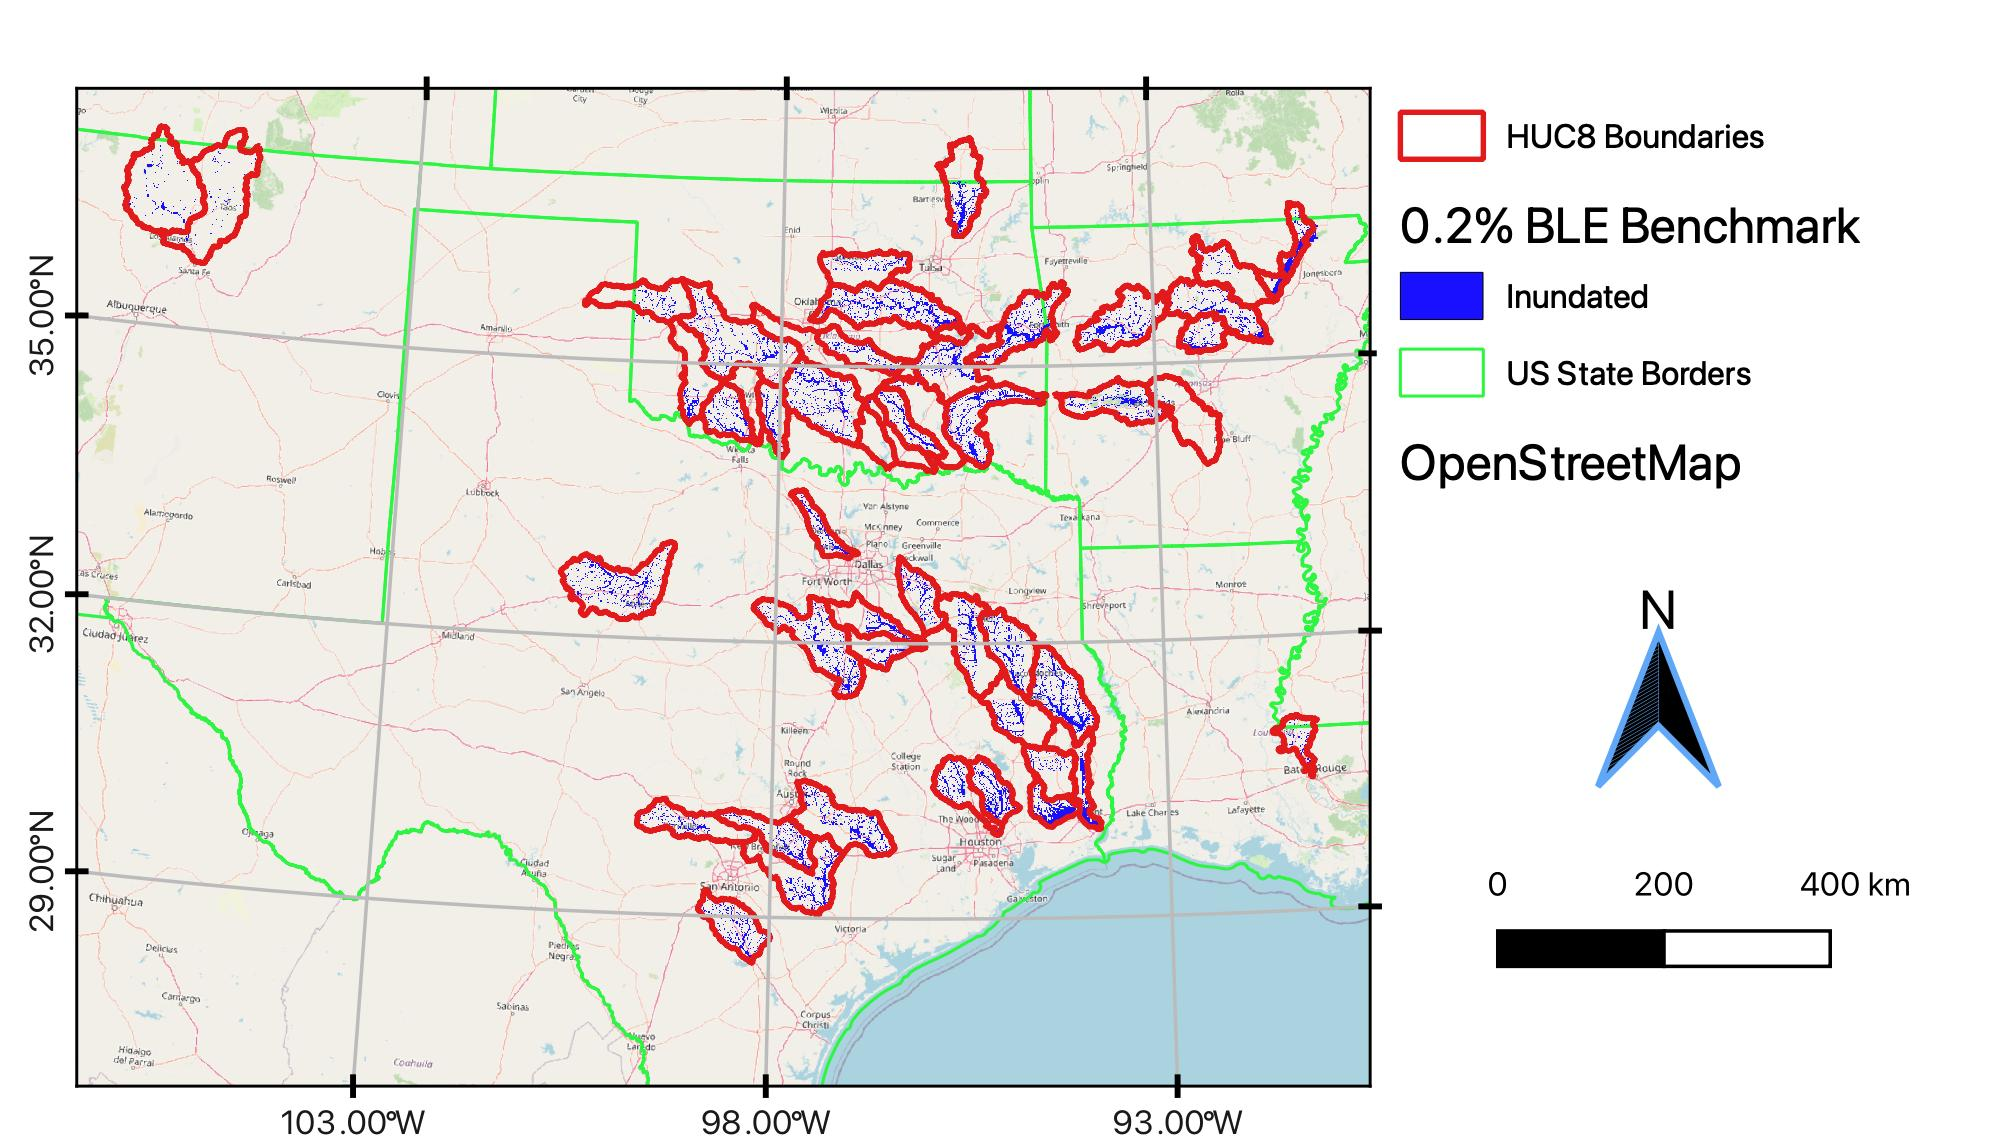
\includegraphics[scale=1.0]{figures/all_ble_maps.jpg}
\caption{
Shows 185 thousand \DIFdelbeginFL \DIFdelFL{square km }\DIFdelendFL \DIFaddbeginFL \DIFaddFL{$km^2$ }\DIFaddendFL of modeled areas for \DIFaddbeginFL \DIFaddFL{the Base Level Engineering (}\DIFaddendFL BLE\DIFaddbeginFL \DIFaddFL{) }\DIFaddendFL domain of 49 HUC8s across \DIFdelbeginFL \DIFdelFL{9 }\DIFdelendFL \DIFaddbeginFL \DIFaddFL{nine }\DIFaddendFL states \DIFaddbeginFL \DIFaddFL{at 0.2\% recurrence magnitude for flow rates}\DIFaddendFL .
\DIFdelbeginFL \DIFdelFL{This dataset }\DIFdelendFL \DIFaddbeginFL \DIFaddFL{BLE maps are produced }\DIFaddendFL for \DIFaddbeginFL \DIFaddFL{two recurrence flows, }\DIFaddendFL 1\% \DIFaddbeginFL \DIFaddFL{(100 yr) }\DIFaddendFL and 0.2\% \DIFdelbeginFL \DIFdelFL{recurrence flows were }\DIFdelendFL \DIFaddbeginFL \DIFaddFL{(500 yr), using 1D HEC-RAS models.
The maps are }\DIFaddendFL used as benchmarks \DIFaddbeginFL \DIFaddFL{for validation purposes of OWP FIM}\DIFaddendFL .
}
\label{fig:all_ble_maps}
\end{figure}
%
\DIFdelbegin %DIFDELCMD < \begin{figure}[h!]
%DIFDELCMD < %%%
\DIFdelendFL \DIFaddbeginFL \begin{figure}[H]
\DIFaddendFL \centering
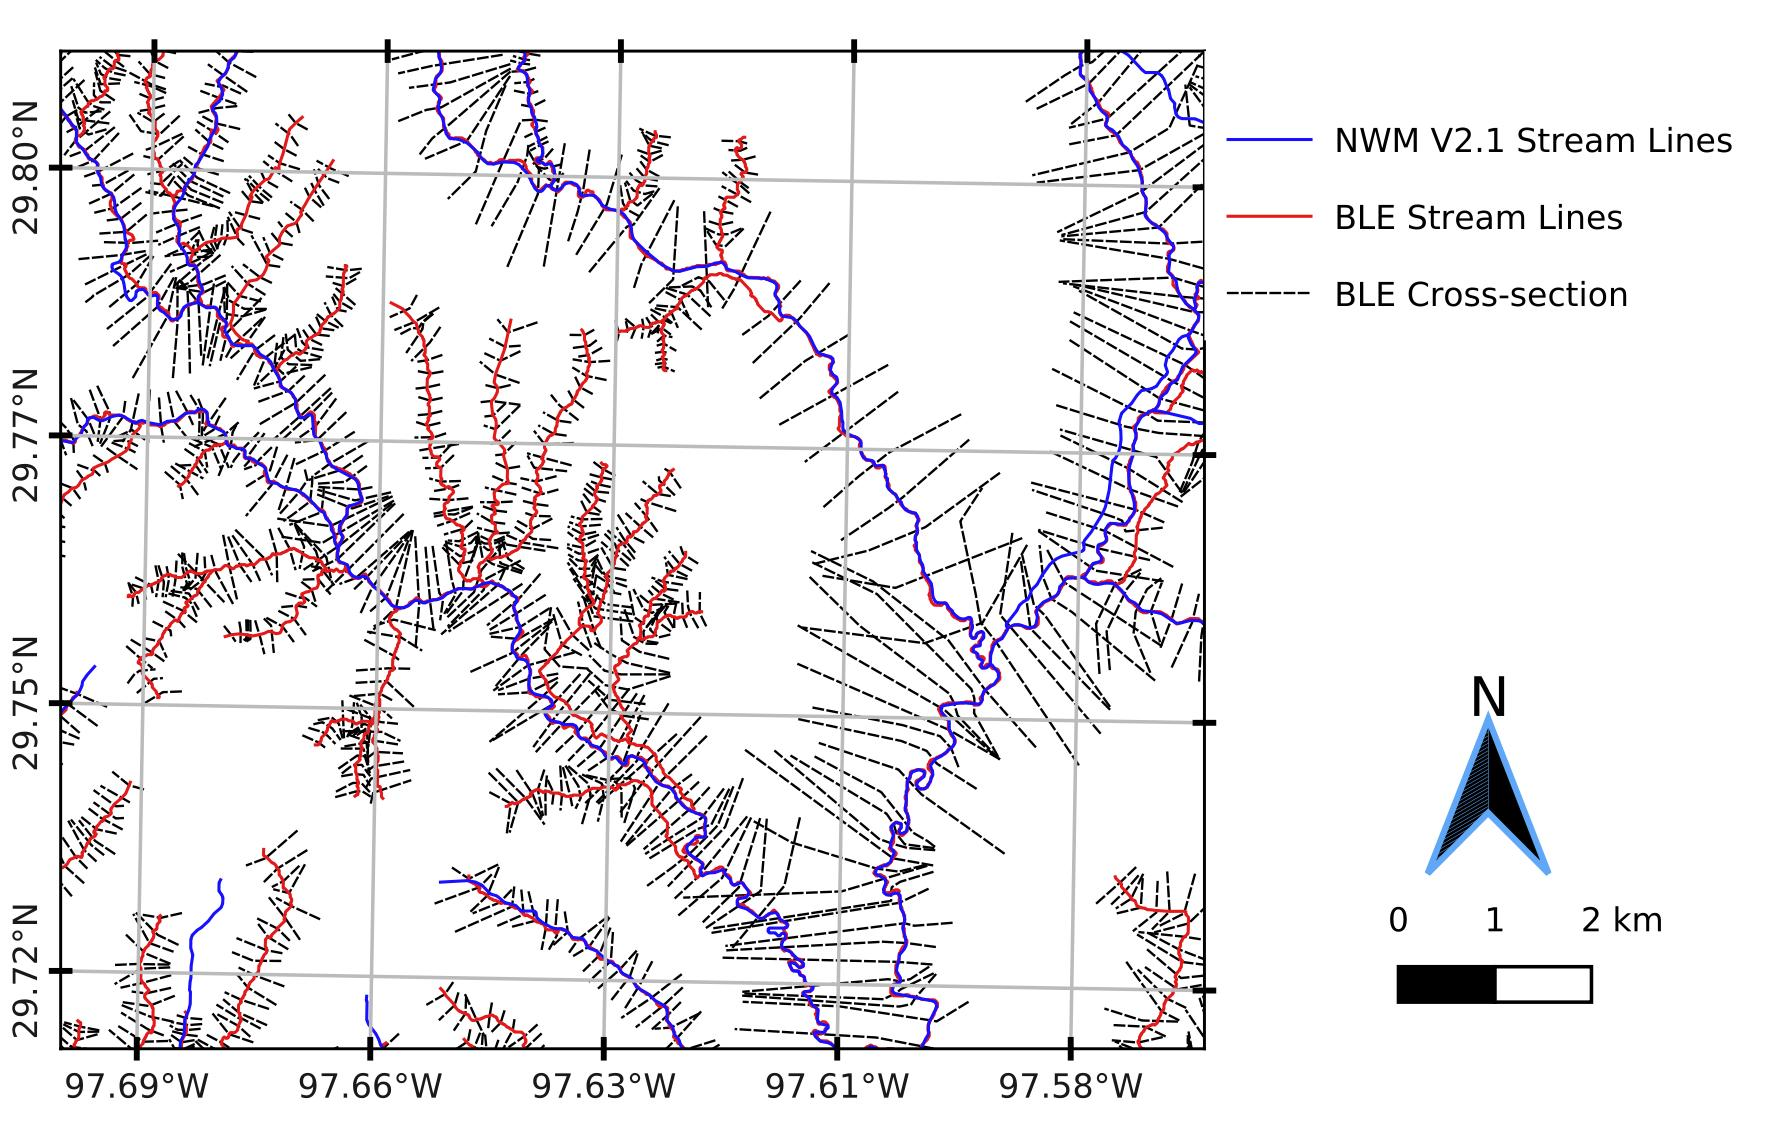
\includegraphics[scale=1.0]{figures/ble_evaluation_method.jpg}
\caption{
Illustrates Base Level Engineering (BLE) cross sections and stream lines \DIFdelbeginFL \DIFdelFL{. The BLE stream network, which is denser than }\DIFdelendFL \DIFaddbeginFL \DIFaddFL{at }\DIFaddendFL the \DIFdelbeginFL \DIFdelFL{NWM V2.1 stream lines, is also shown}\DIFdelendFL \DIFaddbeginFL \DIFaddFL{HUC8 12100203 near the confluences of West Fork Plum Creek and Clear Fork Plum Creek with Plum Creek}\DIFaddendFL .
BLE cross sections are intersected with NWM reaches and the median recurrence discharge for 1\% and 0.2\% levels are selected per NWM \DIFdelbeginFL \DIFdelFL{reach}\DIFdelendFL \DIFaddbeginFL \DIFaddFL{V2.1 Full Resolution (FR) stream lines}\DIFaddendFL .
\DIFaddbeginFL \DIFaddFL{Additionally, we illustrate the NWM V2.1 catchments to provide a sense of how many cross-sections may intersect a given NWM flowline.
The BLE stream network is also shown which is denser than the NWM V2.1 stream lines meaning there are several lower order streams represented in the BLE stream network that are not in the NWM V2.1 stream lines.
This creates additional inundation areas in the validation data that are not modeled with our HAND based FIMs.
}\DIFaddendFL }
\label{fig:ble_evaluation_method}
\end{figure}
%
\DIFaddbegin 

\DIFaddend The metrics employed in this study to evaluate inundation extents include \DIFdelbegin \DIFdel{Critical Success Index (CSI)}\DIFdelend \DIFaddbegin \DIFadd{CSI}\DIFaddend , Probability of Detection (POD), and False Alarm Ratio (FAR) and \DIFaddbegin \DIFadd{are }\DIFaddend presented in Equations \ref{eq:csi}, \ref{eq:pod}, \ref{eq:far}, respectively.
To calculate these secondary metrics, one must define three primary metrics \DIFdelbegin \DIFdel{including }\DIFdelend \DIFaddbegin \DIFadd{starting with }\DIFaddend true positives (TP) which is predicted wet and wet in \DIFaddbegin \DIFadd{the BLE }\DIFaddend benchmark dataset.
The two types of errors consist of false positives (FP), or type I errors, which is dry in \DIFaddbegin \DIFadd{the }\DIFaddend benchmark but predicted wet and false negatives (FN), or type II errors, which is wet in \DIFdelbegin \DIFdel{benchmark by }\DIFdelend \DIFaddbegin \DIFadd{the benchmark but }\DIFaddend predicted dry. 
Lastly, the reader may come across true negatives (TN) which is defined as dry in both the benchmark and predicted datasets.
Maximizing POD indicates a model's ability to detect the given threat of interest, inundation, while minimizing FAR is sought to indicate a models ability in reducing FN errors.
\DIFaddbegin \DIFadd{In other words, POD is an indicator of model skill in inundated regions while FAR is an indicator of model skill in non-inundated regions.
}\DIFaddend Some work by \citeA{gerapetritis2004behavior} \DIFdelbegin \DIFdel{while at the NWM }\DIFdelend denotes CSI a good proxy for measuring a forecasting system's utility in protecting life and property and has been shown to be optimized mathematically when $POD = 1 - FAR$.
\DIFaddbegin \DIFadd{We use all three secondary metrics here to add value to the discussion while avoiding aggregating away the meaning of all four primary metrics.
}

\DIFaddend While these metrics are commonly employed in the evaluation of FIM and binary weather prediction communities in general, they do come with some notable limitations including frequency dependence in the case of CSI and FAR \cite{gerapetritis2004behavior,stephens2014problems,schaefer1990critical,jolliffe2012forecast}.
Thus, frequency dependent statistics should be used with caution when comparing across sites with varying frequencies. 
Lastly, approximately \DIFdelbegin \DIFdel{6 }\DIFdelend \DIFaddbegin \DIFadd{six }\DIFaddend HUC8s do not have NWM MS reaches thus we imputed the metrics for FR for these sites as the best available forecasting capability \DIFaddbegin \DIFadd{to compare GMS metrics to}\DIFaddend .
%
\begin{linenomath*}
\begin{equation}
\label{eq:csi}
CSI = \frac{TP}{TP + FN + FP}
\end{equation}
\end{linenomath*}
%
\begin{linenomath*}
\begin{equation}
\label{eq:pod}
POD = \frac{TP}{TP + FN}
\end{equation}
\end{linenomath*}
%
\begin{linenomath*}
\begin{equation}
\label{eq:far}
FAR = \frac{FP}{TP + FP}
\end{equation}
\end{linenomath*}
%
 %
% Results
\clearpage % this clears figures before references
%%%%%%%%%%%%%%%%%%%%%%%%%%%%%%%%%%%%%%%%%%%%%%%%%%%%%%%%
%%%%%%%%%%%%%%%%%%%%%%%%%%%%%%%%%%%%%%%%%%%%%%%%%%%%%%%%
\section{Results}
\label{sec:results}
%%%%%%%%%%%%%%%%%%%%%%%%%%%%%%%%%%%%%%%%%%%%%%%%%%%%%%%%
%%%%%%%%%%%%%%%%%%%%%%%%%%%%%%%%%%%%%%%%%%%%%%%%%%%%%%%%
%
%%%%%%%%%%%%%%%%%%%%%%%%%%%%%%%%%%%%%%%%%%%%%%%%%%%%%%%%
\subsection{\DIFaddbegin \DIFadd{Flood }\DIFaddend Mapping Performance}
\DIFdelbegin %DIFDELCMD < \label{ssec:mapping_performance}
%DIFDELCMD < %%%
\DIFdelend \DIFaddbegin \label{ssec:flood_mapping_performance}
\DIFaddend %%%%%%%%%%%%%%%%%%%%%%%%%%%%%%%%%%%%%%%%%%%%%%%%%%%%%%%%
%
We produced FIMs for the entire BLE domain within the 49 HUC8 areas across several states in the south central US. 
The forecasted FIMs using the discharges for the 1\% (100 year) and 0.2\% (500 year) recurrence flows directly from HEC-RAS were used to avoid noise and errors from hydrological processes.
We computed the statistics\DIFdelbegin \DIFdel{(}\DIFdelend \DIFaddbegin \DIFadd{, }\DIFaddend CSI, POD, and FAR\DIFdelbegin \DIFdel{) }\DIFdelend \DIFaddbegin \DIFadd{, }\DIFaddend for both 100 and 500 year events for Mannings N set to 0.06 and 0.12.
\DIFaddbegin \DIFadd{These results are presented in Figure \ref{fig:violin_plot} as violin plots and in Table \ref{tab:aggregate_metrics} as aggregated metrics with the results for MS and GMS presented as percentage changes from their respective FR values.
To be more specific, Table \ref{tab:aggregate_metrics} sums the primary metrics, TP, FP, FN, and TN, across all HUC8s then recomputes the secondary metrics which was done to better account for large variances in HUC8 size.
The same trends discussed below are consistent across both reporting methods (Figure \ref{fig:violin_plot} and Table \ref{tab:aggregate_metrics}).
}

\DIFaddend The distribution of these \DIFdelbegin \DIFdel{statistics }\DIFdelend \DIFaddbegin \DIFadd{flood extent metrics }\DIFaddend can be examined in Figure \ref{fig:violin_plot} as violin plots.
Each half of a violin plot represents the kernel density estimation (KDE) for a given model (FR, MS, GMS), \DIFdelbegin \DIFdel{given }\DIFdelend Manning's n value (0.06, 0.12), \DIFdelbegin \DIFdel{and given }\DIFdelend recurrence interval (1\%, 0.2\%), and performance metric (CSI, POD, FAR).
\DIFdelbegin \DIFdel{We also denote trend lines }\DIFdelend \DIFaddbegin \DIFadd{For example, let's examine the violin plot for the row marked CSI and column for Manning's n = 0.06.
This sub-figure shows the CSI distributions across all 49 HUC8s when Manning's n is set to 0.06.
Each independent, whole violin represents the HUC8 metric value distribution of FR, MS, or GMS while each half of the violin represents the distribution of that data divided up by magnitude (blue for 100 yr and orange for 500 yr).
The horizontal dashed and dotted lines represent the 25th, 50th, and 75th percentiles from bottom to top, respectively.
Additionally, we show trend lines symbolized in green that }\DIFaddend for each metric and Manning's n \DIFdelbegin \DIFdel{setting as well as their respective slope estimate and one-tailed }\DIFdelend \DIFaddbegin \DIFadd{combination denotes the best fit line for the three methods (FR, MS, and GMS).
To avoid having two trend lines per sub-figure, we elected to aggregate the two magnitudes together as they tend to observe similar trends across the three models.
The slope of each trend line is quantified in the figure by its $\beta_1$ value and the }\DIFaddend p-value \DIFdelbegin \DIFdel{denoting the level of significance of the trend }\DIFdelend \DIFaddbegin \DIFadd{for that statistic which tests the significance of that trend (deviation from a zero sloped trend line)}\DIFaddend .

\DIFdelbegin \DIFdel{Aggregating the metrics in the method above treats each HUC8 as it's own unit and does little to consider the size differences of the HUCs.
In an opposing aggregation method, we illustrate in Table \ref{tab:aggregate_metrics}  the CSI, POD}\DIFdelend %DIF >  Interpretation of metrics
\DIFaddbegin \DIFadd{Both Figure \ref{fig:violin_plot} and Table \ref{tab:aggregate_metrics} contain a fair amount of information that is central to the objectives of this study.
As previously stated in Section \ref{ssec:evaluation}, we consider CSI as a general proxy for the skill of the inundation extents with POD denoting skill on inundated areas and FAR indicating skill on non-inundated areas.
Again, the main objective of the study is to introduce how computing HAND with disaggregated stream networks to those with unit stream order can enhance the fidelity of FIMs by capturing fluvial inundation from multiple sources as opposed to that of just the nearest drainage line.
As can be seen in Figure \ref{fig:violin_plot} and Table \ref{tab:aggregate_metrics}, CSI generally increases from FR to MS and MS to GMS for both sets of Manning's n values and flood magnitudes.
This increase is primarily driven by an increase in POD thus generally increasing the probability of correctly detecting inundation.
Also, we note that FAR is somewhat, albeit marginally, decreased from FR to MS and MS to GMS for both sets of Manning's n values and flood magnitudes.
The increases in CSI and POD as well as the decreases in FAR with respect to the methods, FR, MS, and GMS, are not only observed among the trend lines but also in the 25th}\DIFaddend , \DIFdelbegin \DIFdel{and FARrecomputed for }\DIFdelend \DIFaddbegin \DIFadd{50th, and 75th percentiles (Figure \ref{fig:violin_plot}).
So overall and in other words, the broader distribution of HUC8s improves across the three methods.
Due to the means by which FIM is produced utilizing FR, MS, and GMS, we can say that the more we derive HAND on networks of unit stream order and mosaic the resulting FIMs, the better those FIMs perform.
We move more details on the relationship between stream order and FIM skill to the Discussion section (Section \ref{sec:discussion}).
}

\DIFadd{Additional noteworthy trends in Figure \ref{fig:violin_plot} center around the all-around better performance of FIMs for those of higher Manning's n values and recurrence flows.
The higher Manning's n value enhances performance for both recurrence intervals across all models which seems to better agree with the value of 0.11 used in the BLE model \mbox{%DIFAUXCMD
\cite{fema2021base,fema2021estimated}}\hskip0pt%DIFAUXCMD
.
Most of this improvement is driven by significant increases in POD, but unfortunately, it also leads to a significant amount of over-prediction as observed by the increase in FAR.
More work can be invested to better regionalize Manning's n values for FIM purposes with HAND.
We also observe additional trends associated with the magnitude or recurrence interval of }\DIFaddend the \DIFdelbegin \DIFdel{entire domain using the sum of all the TPs, FPs, and FNs.
}\DIFdelend \DIFaddbegin \DIFadd{flow rates used with the higher flow rates exhibiting better overall CSI, POD, and FAR values than the lower, 100 yr magnitude.
We introduce in the Discussion (Section \ref{sec:discussion}) that this skill premium exhibited by higher flow events could be due higher quality elevation data in regions that are not described as bathymetric areas.
}\DIFaddend %
\DIFdelbegin %DIFDELCMD < \begin{figure}[h!]
%DIFDELCMD < %%%
\DIFdelendFL \DIFaddbeginFL \begin{figure}[H]
\DIFaddendFL \centering
\DIFdelbeginFL %DIFDELCMD < 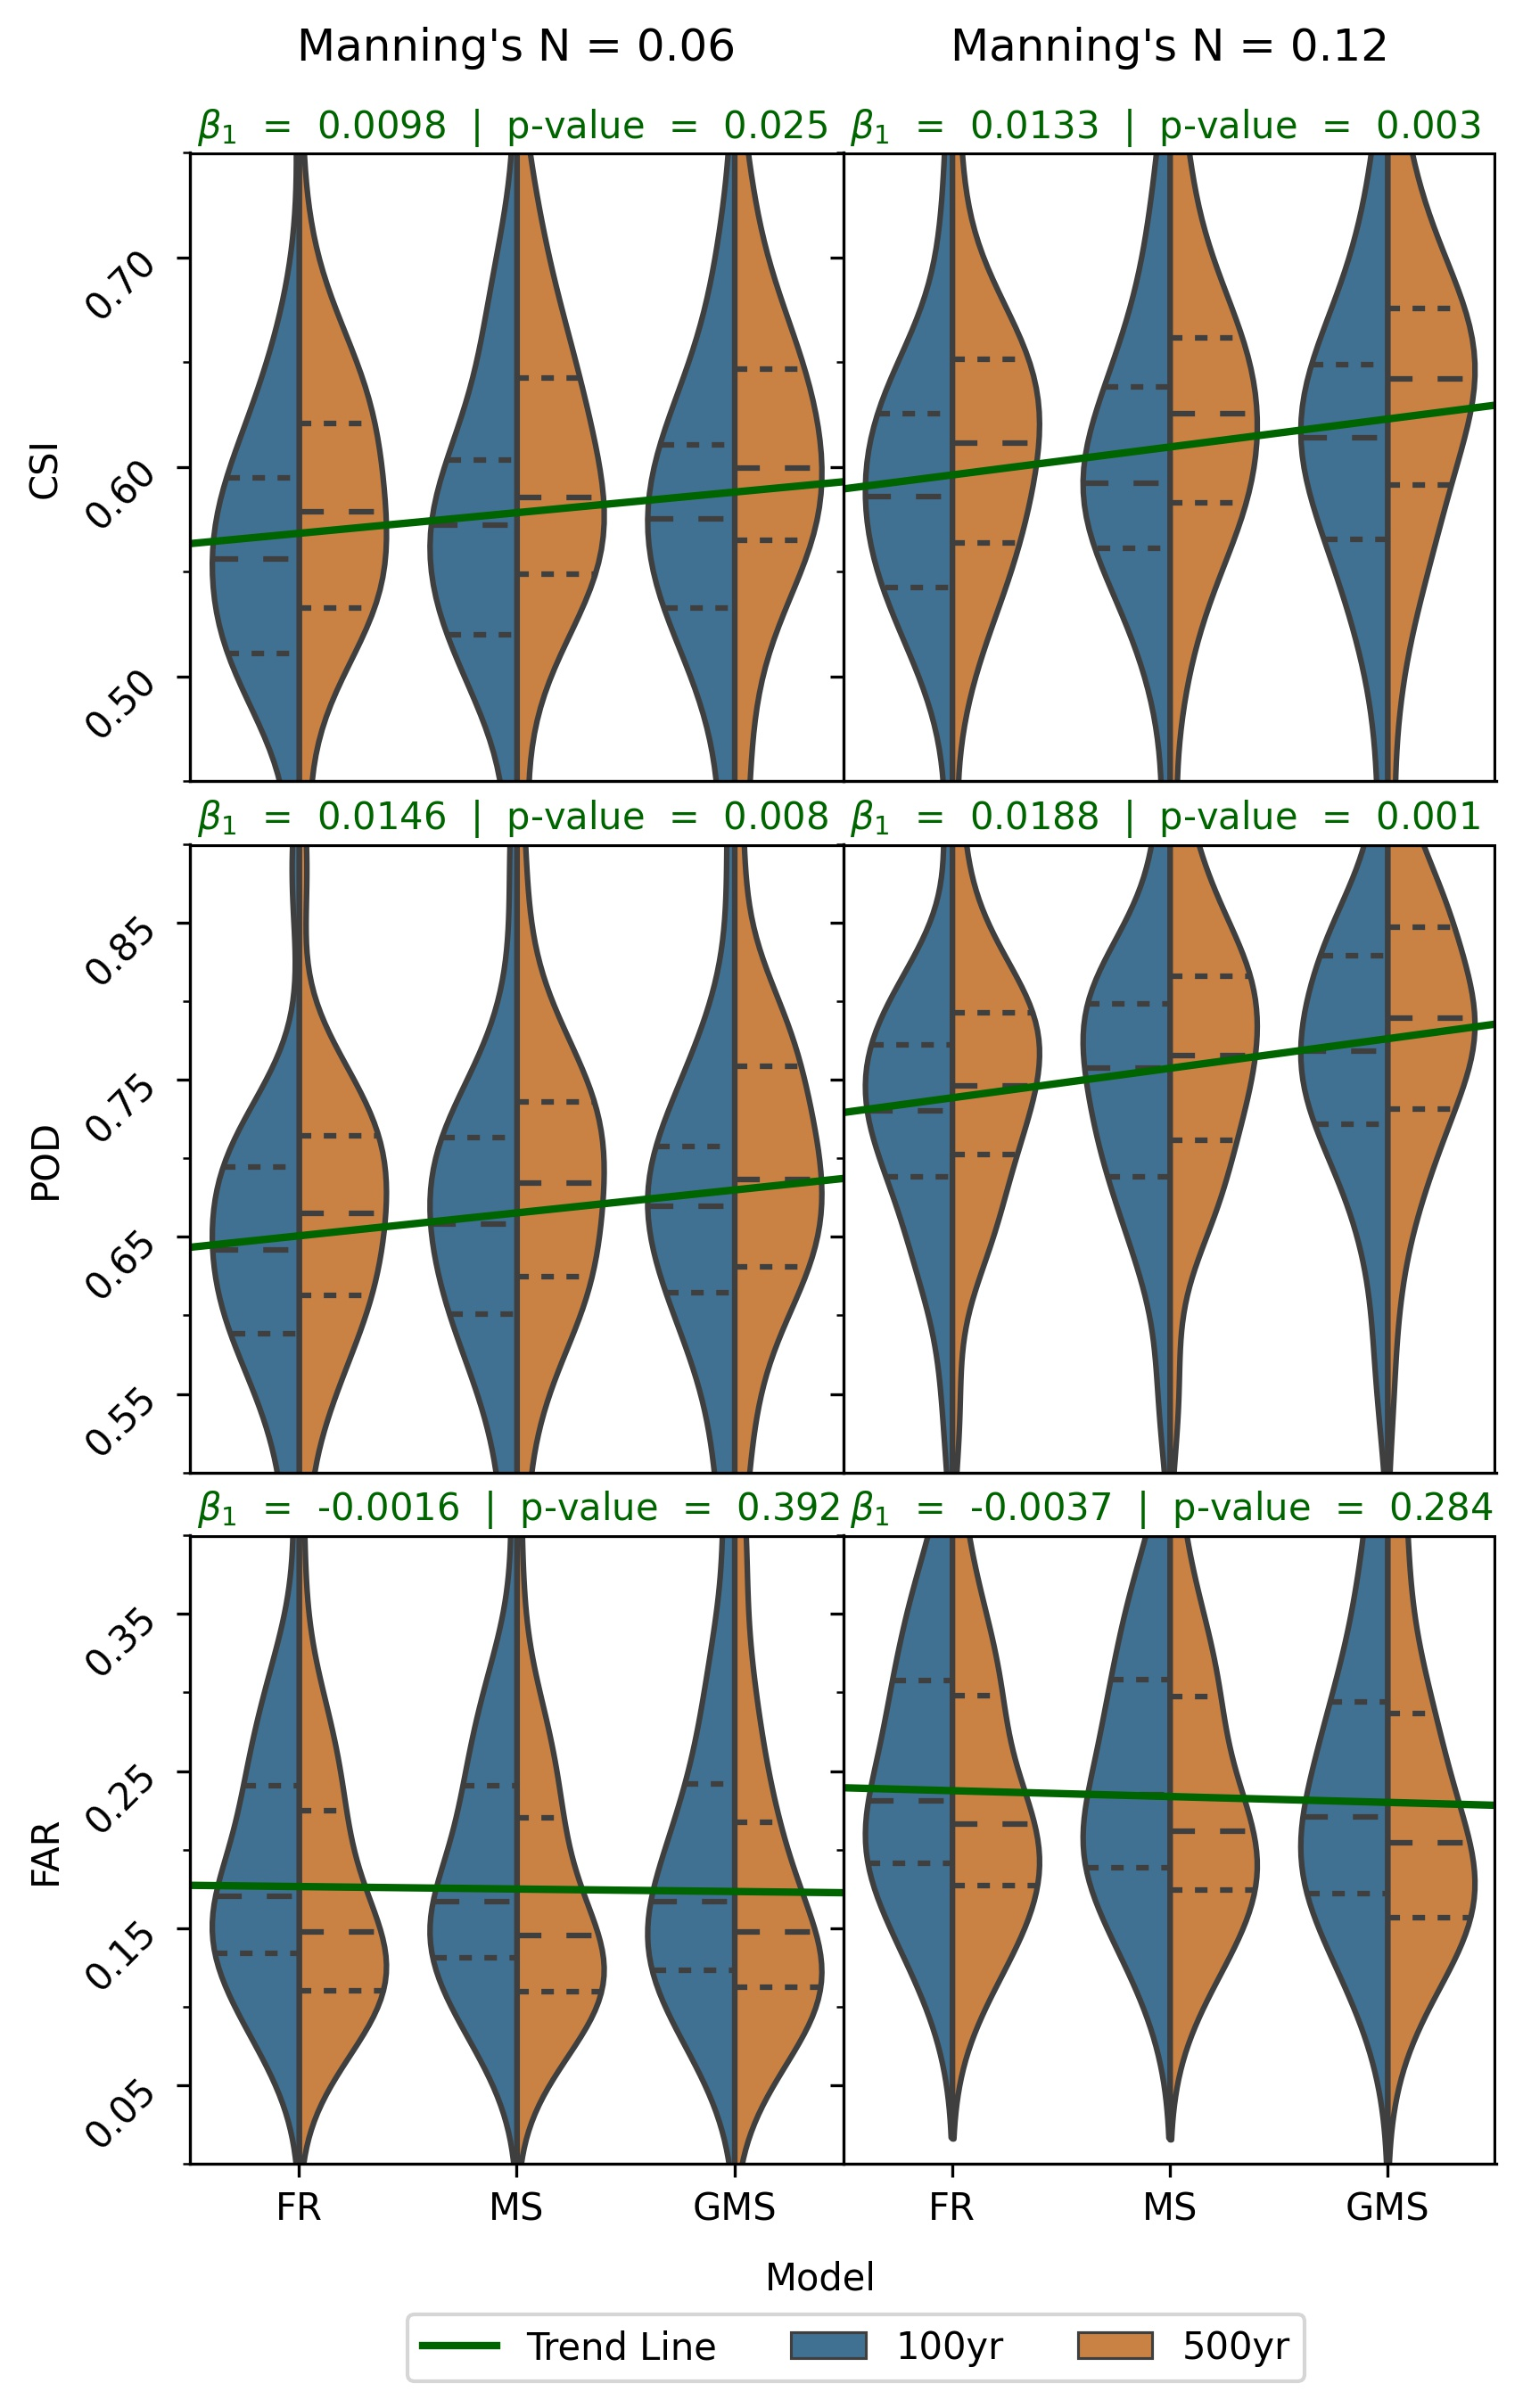
\includegraphics[scale=0.9]{figures/violin_plots.jpg}
%DIFDELCMD < %%%
\DIFdelendFL \DIFaddbeginFL 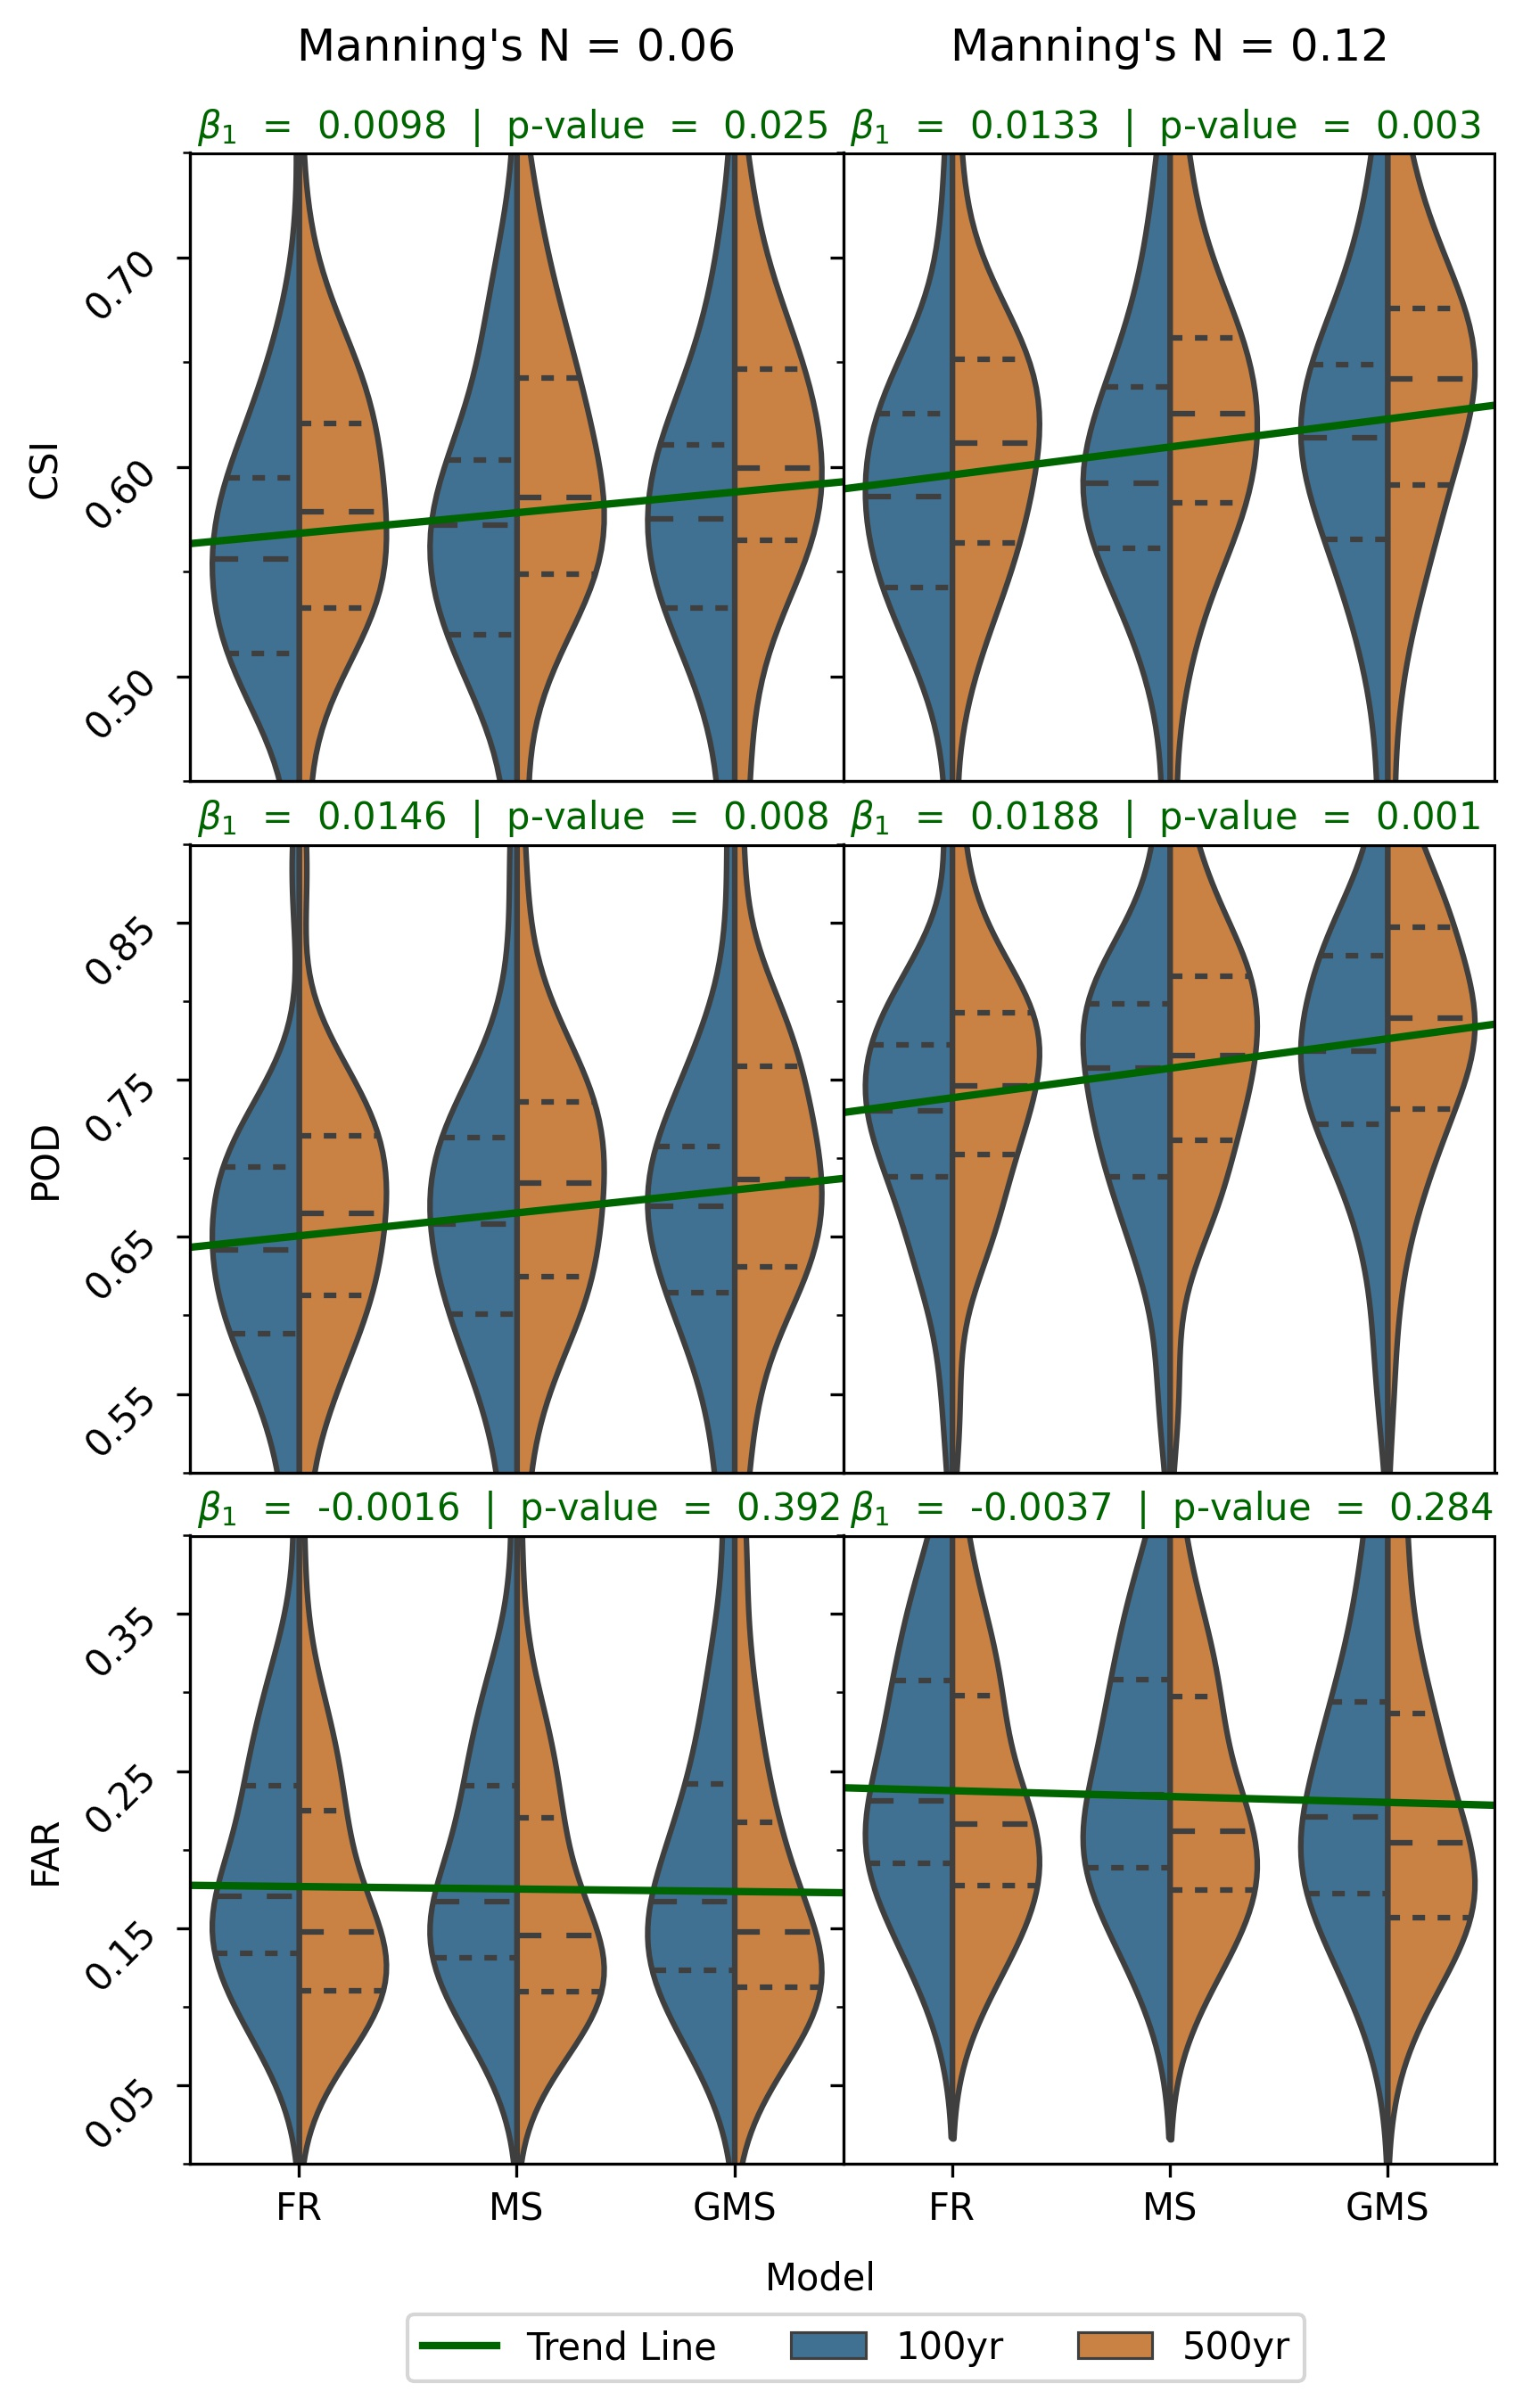
\includegraphics[scale=0.8]{figures/violin_plots.jpg}
\DIFaddendFL \caption{Shows kernel density estimation of the distributions (sample size = 49) for 1\% (100 year) and 0.2\% (500 year) along with horizontal, dashed lines for the 25th, 50th, and 75th percentiles (in order from bottom to top).
The sub-figures separate the combination of three metrics (CSI, POD, and FAR) for two settings of Manning's n (0.06 and 0.12).
Trend lines for each \DIFdelbeginFL \DIFdelFL{metric - Mannings }\DIFdelendFL combination \DIFaddbeginFL \DIFaddFL{of metric and Manning's n }\DIFaddendFL are shown (sample size = 294) along with associated slope and p-value of slope testing one-tailed significance.}
\label{fig:violin_plot}
\end{figure}
%
\DIFdelbegin %DIFDELCMD < \begin{table}[h!]
%DIFDELCMD < %%%
\DIFdelendFL \DIFaddbeginFL \begin{table}[H]
\DIFaddendFL \caption{ Recomputed CSI, POD, and FAR using the primary metrics, TPs, FPs, and FNs, aggregated \DIFdelbeginFL \DIFdelFL{for }\DIFdelendFL \DIFaddbeginFL \DIFaddFL{to the }\DIFaddendFL BLE domain.
         The \DIFaddbeginFL \DIFaddFL{values for MS and GMS methods are expressed in percentage change (\%) from their respective values with the same Manning's n, magnitude, and metric combination in the Full Resolution (FR) method columns.
         The }\DIFaddendFL best value across models is highlighted in bold.}
\label{tab:aggregate_metrics}
\centering
%\begin{tabular}{|p{2cm}|p{2cm}|p{2cm}|p{2cm}|}
\begin{tabular}{|c|c||c|c|c|c|c|c|}
\hline
\multirow{2}{*}{Metric} & \multirow{2}{*}{Manning's n} & \multicolumn{2}{|c|}{FR} & \DIFdelbeginFL %DIFDELCMD < \multicolumn{2}{|c|}{MS} %%%
\DIFdelendFL \DIFaddbeginFL \multicolumn{2}{|c|}{\shortstack{MS\\(\% Change)}} \DIFaddendFL & \DIFdelbeginFL %DIFDELCMD < \multicolumn{2}{|c|}{GMS} %%%
\DIFdelendFL \DIFaddbeginFL \multicolumn{2}{|c|}{\shortstack{GMS\\(\% Change)}} \DIFaddendFL \\
%DIF > \multirow{2}{*}{Metric} & \multirow{2}{*}{Manning's n} & \multicolumn{2}{|c|}{FR} & \multicolumn{2}{|c|}{\shortstack{MS\\(\% Change)}} & \multicolumn{2}{|c|}{\shortstack{GMS\\(\% Change)}} \\
\cline{3-8}
  &  & \DIFdelbeginFL \DIFdelFL{100yr }\DIFdelendFL \DIFaddbeginFL \DIFaddFL{100 yr }\DIFaddendFL & \DIFdelbeginFL \DIFdelFL{500yr }\DIFdelendFL \DIFaddbeginFL \DIFaddFL{500 yr }\DIFaddendFL & \DIFdelbeginFL \DIFdelFL{100yr }\DIFdelendFL \DIFaddbeginFL \DIFaddFL{100 yr }\DIFaddendFL & \DIFdelbeginFL \DIFdelFL{500yr }\DIFdelendFL \DIFaddbeginFL \DIFaddFL{500 yr }\DIFaddendFL & \DIFdelbeginFL \DIFdelFL{100yr }\DIFdelendFL \DIFaddbeginFL \DIFaddFL{100 yr }\DIFaddendFL & \DIFdelbeginFL \DIFdelFL{500yr }\DIFdelendFL \DIFaddbeginFL \DIFaddFL{500 yr }\DIFaddendFL \\
\hline
\multirow{2}{*}{CSI} & 0.06 & 0.5576 & 0.5839 & \DIFdelbeginFL \DIFdelFL{0.5717 }\DIFdelendFL \DIFaddbeginFL \DIFaddFL{2.53 }\DIFaddendFL & \DIFdelbeginFL \DIFdelFL{0.5990 }\DIFdelendFL \DIFaddbeginFL \DIFaddFL{2.59 }\DIFaddendFL & \textbf{\DIFdelbeginFL \DIFdelFL{0.5796}\DIFdelendFL \DIFaddbeginFL \DIFaddFL{3.95}\DIFaddendFL } & \textbf{\DIFdelbeginFL \DIFdelFL{0.6075}\DIFdelendFL \DIFaddbeginFL \DIFaddFL{4.04}\DIFaddendFL } \\
\cline{2-8}
  & 0.12 & 0.5915 & 0.6149 & \DIFdelbeginFL \DIFdelFL{0.6054 }\DIFdelendFL \DIFaddbeginFL \DIFaddFL{2.35 }\DIFaddendFL & \DIFdelbeginFL \DIFdelFL{0.6288 }\DIFdelendFL \DIFaddbeginFL \DIFaddFL{2.26 }\DIFaddendFL & \textbf{\DIFdelbeginFL \DIFdelFL{0.6182}\DIFdelendFL \DIFaddbeginFL \DIFaddFL{4.51}\DIFaddendFL } & \textbf{\DIFdelbeginFL \DIFdelFL{0.6435}\DIFdelendFL \DIFaddbeginFL \DIFaddFL{4.65}\DIFaddendFL } \\
\hline
\multirow{2}{*}{POD} & 0.06 & 0.6354 & 0.6575 & \DIFdelbeginFL \DIFdelFL{0.6524 }\DIFdelendFL \DIFaddbeginFL \DIFaddFL{2.68 }\DIFaddendFL & \DIFdelbeginFL \DIFdelFL{0.6755 }\DIFdelendFL \DIFaddbeginFL \DIFaddFL{2.74 }\DIFaddendFL & \textbf{\DIFdelbeginFL \DIFdelFL{0.6633}\DIFdelendFL \DIFaddbeginFL \DIFaddFL{4.39}\DIFaddendFL } & \textbf{\DIFdelbeginFL \DIFdelFL{0.6863}\DIFdelendFL \DIFaddbeginFL \DIFaddFL{4.38}\DIFaddendFL } \\
\cline{2-8}
  & 0.12 & 0.7255 & 0.7446 & \DIFdelbeginFL \DIFdelFL{0.7460 }\DIFdelendFL \DIFaddbeginFL \DIFaddFL{2.83 }\DIFaddendFL & \DIFdelbeginFL \DIFdelFL{0.7648 }\DIFdelendFL \DIFaddbeginFL \DIFaddFL{2.71 }\DIFaddendFL & \textbf{\DIFdelbeginFL \DIFdelFL{0.7606}\DIFdelendFL \DIFaddbeginFL \DIFaddFL{4.84}\DIFaddendFL } & \textbf{\DIFdelbeginFL \DIFdelFL{0.7810}\DIFdelendFL \DIFaddbeginFL \DIFaddFL{4.89}\DIFaddendFL } \\
\hline
\multirow{2}{*}{FAR} & 0.06 & 0.1800 & 0.1609 & \DIFdelbeginFL \DIFdelFL{0.1787 }\DIFdelendFL \DIFaddbeginFL \DIFaddFL{-0.72 }\DIFaddendFL & \textbf{\DIFdelbeginFL \DIFdelFL{0.1589}\DIFdelendFL \DIFaddbeginFL \DIFaddFL{-1.24}\DIFaddendFL } & \textbf{\DIFdelbeginFL \DIFdelFL{0.1778}\DIFdelendFL \DIFaddbeginFL \DIFaddFL{-1.22}\DIFaddendFL } & \textbf{\DIFdelbeginFL \DIFdelFL{0.1589}\DIFdelendFL \DIFaddbeginFL \DIFaddFL{-1.24}\DIFaddendFL } \\
\cline{2-8}
  & 0.12 & 0.2379 & 0.2208 & \DIFdelbeginFL \DIFdelFL{0.2374 }\DIFdelendFL \DIFaddbeginFL \DIFaddFL{-0.21 }\DIFaddendFL & \DIFdelbeginFL \DIFdelFL{0.2204 }\DIFdelendFL \DIFaddbeginFL \DIFaddFL{-0.18 }\DIFaddendFL & \textbf{\DIFdelbeginFL \DIFdelFL{0.2324}\DIFdelendFL \DIFaddbeginFL \DIFaddFL{-2.31}\DIFaddendFL } & \textbf{\DIFdelbeginFL \DIFdelFL{0.2148}\DIFdelendFL \DIFaddbeginFL \DIFaddFL{-2.72}\DIFaddendFL } \\
\hline
\end{tabular}
\end{table}
%
%DIF <  Interpretation of metrics
\DIFdelbegin \DIFdel{From Figure \ref{fig:violin_plot} and Table \ref{tab:aggregate_metrics}, we denote several meaningful trends. 
Using CSI as an overall proxy for skill of the FIM, we note that generally speaking the skill is correlated with a reduction of the stream orders of the processing units used for HAND.
In other words, the more we derive HAND on networks of unit drainage density and mosaic the resulting FIMs, the better those FIMs perform.
While this trend is evident for both sets of Manning's n values, the trend is slightly more significant for the higher value of 0.12.
Other trends related to this Figure include the general performance premium for 0.2\% events as opposed to lower 1\% events.
We also note how the higher Manning's n value enhances performance for both of these recurrence intervals across all models.
}%DIFDELCMD < 

%DIFDELCMD < %%%
\DIFdel{Dissecting the improvements and trends presented in the previous paragraph comes down mostly to improvement in POD or a reduction in absolute amount of FNs.
POD being the primary driver in skill enhancement is evident across models by comparing the slope of the POD lines with the slope of the FAR lines.
Even though aggregating metrics by HUC8 yields a statistically zero trend, one does see a slight reduction in FAR across models that reduce HAND's maximum stream order.
Additionally, we note that POD is a primary driver in enhancing performance across Manning's n values as well.
This significant improvement comes at a cost of false alarms as the FAR increases significantly across Manning's n values.
%DIF < 
}\DIFdelend %%%%%%%%%%%%%%%%%%%%%%%%%%%%%%%%%%%%%%%%%%%%%%%%%%%%%%%%
\subsection{Computational Performance}
\label{ssec:compuational_performance}
%%%%%%%%%%%%%%%%%%%%%%%%%%%%%%%%%%%%%%%%%%%%%%%%%%%%%%%%
%
The NFIE experiments were able to produce HAND for 331 HUC6's in 1.34 CPU years \cite{liu2016cybergis} and estimates using work from \citeA{djokic2019arc} put producing HAND at the FR NWM at 0.55 CPU years. 
For our work, we were able to produce HAND at the full NWM resolution in 0.13 CPU years which represents a substantial speed-up compared to previous works.
For the MS resolution\DIFdelbegin \DIFdel{an additional, }\DIFdelend \DIFaddbegin \DIFadd{, an additional }\DIFaddend 0.05 CPU years is required on top of this bringing the total to about 0.18 CPU years to produce 2,188 HUC8s that span additional areas not covered in previous HAND versions including Hawaii and Puerto Rico.
GMS which generalizes HAND production to \DIFdelbegin \DIFdel{level path }\DIFdelend \DIFaddbegin \DIFadd{the LP }\DIFaddend scale adds a significant amount of CPU time to the process bringing the estimate total to about 1.17 CPU years.
%
 %
% Discussion
\clearpage % this clears figures before references
%%%%%%%%%%%%%%%%%%%%%%%%%%%%%%%%%%%%%%%%%%%%%%%%%%%%%%%%
%%%%%%%%%%%%%%%%%%%%%%%%%%%%%%%%%%%%%%%%%%%%%%%%%%%%%%%%
\section{Discussion}
\label{sec:discussion}
%%%%%%%%%%%%%%%%%%%%%%%%%%%%%%%%%%%%%%%%%%%%%%%%%%%%%%%%
%%%%%%%%%%%%%%%%%%%%%%%%%%%%%%%%%%%%%%%%%%%%%%%%%%%%%%%%
%
Overall, \DIFdelbegin \DIFdel{we note a positive relationship between FIM skill and a reduction of the }\DIFdelend \DIFaddbegin \DIFadd{the main observation of this study was how FIM performance can be improved by reducing the Horton-Strahler }\DIFaddend stream order of the \DIFdelbegin \DIFdel{stream network we use to derive the HAND datasets}\DIFdelend \DIFaddbegin \DIFadd{target stream network used for HAND computation}\DIFaddend .
Most of this change is accounted for by \DIFdelbegin \DIFdel{increasing POD }\DIFdelend \DIFaddbegin \DIFadd{substantially increasing POD and inundation extents in some areas }\DIFaddend thus reducing FNs\DIFdelbegin \DIFdel{especially along higher order rivers with higher flow magnitudes.
We }\DIFdelend \DIFaddbegin \DIFadd{.
We believe, as we later argue, that the increase in POD is primarily driven by an increase in the catchment sizes that is inherently enabled by dividing up the stream network into independent stream networks of unit stream order.
Additionally, we }\DIFaddend note that reducing \DIFdelbegin \DIFdel{stream order does in turn suffer from diminishing returns in which the increase in mapping skill for applying stream order reduction to roughly 4-5\% of }\DIFdelend \DIFaddbegin \DIFadd{drainage order also has some minor influence on reducing inundation extents in other areas and the rate of false alarms.
We believe that this effect is driven by a change in the stage-discharge relationship where a given streamflow leads to lower river stage values when HAND is computed with target stream networks of unit drainage order.
We seek to explain that these two effects, catchment boundary enlargement and stage-discharge curve lowering, are highly interrelated and cannot be easily detangled.
Lastly, we discuss the diminishing effects on performance that the MS and GMS techniques may have and also any additional effects including enhanced cross-walking abilities.
}

\DIFadd{As evident in }\DIFaddend the \DIFdelbegin \DIFdel{stream network is about the same as }\DIFdelend \DIFaddbegin \DIFadd{results of the study in Section \ref{sec:results}, a sizable amount of the increase in CSI observed by reducing stream order for HAND computation can be attributed to increases in POD.
This can be inferred by close inspection of Figure \ref{fig:violin_plot} and Table \ref{tab:aggregate_metrics} where changes in POD are significantly higher than that of FAR.
%DIF > This intuition is confirmed by previously mentioned work by \citeA{gerapetritis2004behavior} where CSI was shown to be a direct function of both POD and FAR where CSI is maximized when $POD = 1 - FAR$.
Upon investigation of the performance of HAND derived FIM, we note a general increase of catchment sizes for the MS and GMS methods when compared to the FR method as they are now delineated independently of any tributaries that would constrain catchment sizes otherwise.
Additionally, we note significantly less water build up along catchment boundaries especially at the junction of lower order tributaries with lower flow rates and higher order rivers with more flow.
This allows for inundation extents to expand across regions previously encapsulated by catchments of joining reaches in lower flow tributaries.
The water built up along the catchment boundaries can be thought of as a column of water in a cylindrical container (catchment) that has exceeded the elevation of the container's rim which does not represent accurate physics.
}

\DIFadd{Large scale HUC8 level evaluations can fail to demonstrate fine grain enhancements as they aggregate away many changes that are only clear at more local scales.
Future assessments of OWP FIM should consider finer grain evaluation units as well possible impact assessments using asset information such as building footprints to better illustrate fine grain changes in a more relevant manner to stakeholders.
For now, we provide Figure \ref{fig:gms_enhancement} which best illustrates the improvement offered by multi-source fluvial flooding capabilities in a more local context.
The figure is comprised of two agreement rasters for two different HAND based FIMs compared to the validation dataset for a given region with a high flow mainstem (500 yr recurrence flow) running horizontally along the region.
Sub-figure \ref{fig:gms_enhancement}a demonstrates the agreement raster for the FR stream network as well as its respective catchment boundary lines symbolized in white and stream network shown in green.
Inspection of this sub-figure denotes a clear spatial pattern where TPs or areas correctly inundated are pooled alongside catchment boundary lines. 
On the other side of the catchment boundary, one can witness large swaths of FNs that should be inundated. 
The FNs also exhibit a spatial pattern as in they tend to collocate within catchments of the pictured mainstems tributaries.
This sort of behavior was introduced early in }\DIFaddend the \DIFdelbegin \DIFdel{increase for applying stream order reduction to the remaining 95-96\% of the stream network.
This motivates further work in identifying what the optimal coverage of stream order reduction could be and how to parameterize that coverage.
One option could be removing stream orders ones and possibly twos and threes from stream order reduction and simply using the inundation from FR from these areas.
}\DIFdelend \DIFaddbegin \DIFadd{paper and shown qualitatively in Figure \ref{fig:catchment_boundaries_issue}.
}\DIFaddend 

\DIFdelbegin \DIFdel{In analyzing the data}\DIFdelend \DIFaddbegin \DIFadd{As an enhancement, this paper proposes computing HAND for stream networks comprised of level-paths independently of one another.
In sub-figure \ref{fig:gms_enhancement}b, the agreement raster for the GMS technique is illustrated as well as the stream network lines in green.
While the entire mosaiced inundation map from GMS (as described in Section \ref{ssec:inundation_mapping} and Equation \ref{eq:hand_fim_depth}) is used to produce this agreement map, we only show the catchments associated with the mainstem of this region that is shown to follow a clear horizontal path.
Showing all the catchments for the tributaries that were all derived independently would convolute the image.
The main message illustrated here is that the catchments associated with the mainstem of this area significantly increase in size.
Since they are not restricted by the catchments of tributaries that lie in the same drainage areas as those of the mainstem, they extend to include those as well.
The consequence for inundation extents is a general increase in spatial coverage of the river's water which shows to be in much better agreement with the benchmark map.
The TPs are no longer bounded by the catchment lines and allowed to expand to their natural extents.
}

\DIFadd{We note here as a contribution of this study that a major inherent, limitation of HAND is the ``nearest drainage'' constraint or the idea that a given river reach only drains or, in HAND's case, inundates its immediate, unique drainage area or catchment.
In other words, HAND based FIMs are limited to producing fluvial inundation to only their nearest drainage area or catchment.
However, we know that fluvial inundation can be sourced from several streams nearby that also serve as drainage outlets to the area in question.
Generally speaking, drainage areas are known to be hierarchical in nature so a given drainage area for a given outlet point can be decomposed into nested drainage areas for outlet points that lie in the original drainage area.
A perfect example of this are points that lie on tributary reaches closely neighboring a mainstem.
These points lie in the drainage area of reaches in the mainstem but inundation from the mainstem cannot reach these tributary catchments because of the ``nearest'' assumption in HAND.
Hence it's important to state that just like there are different sources of flooding such as fluvial, pluvial, groundwater, reservoir, barrier failure (dam/levee/embankment), and coastal, there can also be multiple sources of a riverine flood.
HAND is only equipped to handle riverine flooding from the nearest drainage line.
Other relevant drainage lines that produce fluvial flood waters are not considered here especially if the routing model used doesn't consider backwater effects.
}

\DIFadd{The remaining portion of the improvement in CSI was found to come from a marginal yet notable reduction in FAR.
Upon investigation of the spatial results in the agreement maps}\DIFaddend , we found \DIFdelbegin \DIFdel{a slight reduction in FAR was detected and more digging pointed to a bias in rating curves }\DIFdelend \DIFaddbegin \DIFadd{some areas of slight reductions in FPs especially where changes in catchment boundaries may have occurred due to the reduction in effective stream order in computing HAND.
These observations pointed to changes in the SRCs }\DIFaddend introduced by stream order reduction \DIFaddbegin \DIFadd{and catchment definition adjustments}\DIFaddend .
Figure \ref{fig:rating_curve_comparison} illustrates the general effect that stream order reduction has on \DIFdelbegin \DIFdel{synthetic rating curves}\DIFdelend \DIFaddbegin \DIFadd{SRCs}\DIFaddend .
Sub-figure \ref{fig:rating_curve_comparison}a shows how the average \DIFdelbegin \DIFdel{rating curves }\DIFdelend \DIFaddbegin \DIFadd{SRCs }\DIFaddend for all reaches for stage values 0 to 25 meters at one-third meter intervals tend to \DIFdelbegin \DIFdel{bias down (}\DIFdelend \DIFaddbegin \DIFadd{shift the curve down }\DIFaddend and to the right \DIFdelbegin \DIFdel{) }\DIFdelend with ever increasing stream order reduction (FR to MS to GMS). 
This bias is more pronounced for GMS since that implements stream order reduction down to the unit level for the entire FR network while MS only does so for 4-5\% of the network.
\DIFaddbegin 

\DIFaddend Attempting to diagnose this bias in the SRC leads one to Equation \ref{eq:reach_averaged_mannings_equation} which shows the reach averaged \DIFdelbegin \DIFdel{synthetic rating curve }\DIFdelend \DIFaddbegin \DIFadd{SRC }\DIFaddend relationship between stage and discharge.
Across the three methods explored, FR, MS, and GMS, one identifies differences in the inputs and outputs and notes no difference in the stages and Manning's n values.
While the channel slope and reach lengths are not exactly the same across methods, their averaged differences are very negligible which only leaves room for deviations in volume and bed area.
Again, volume (V(y) or simply V) is synonymous to reach-averaged cross-sectional area and bed area (B(y) or B) is analogous to reach-averaged hydraulic radius \DIFaddbegin \DIFadd{but these associations only hold when reach length, L, is considered}\DIFaddend .
Discharge, Q, is directly related to volume and inversely related to bed area and each parameter is weighed according to the magnitude of its exponent which are $\frac{5}{3}$ and $\frac{2}{3}$ respectively (see Equation \ref{eq:reach_averaged_mannings_equation}). 
Figures \ref{fig:rating_curve_comparison}b and \DIFaddbegin \DIFadd{\ref{fig:rating_curve_comparison}}\DIFaddend c show how volume and bed area compare across the three methods with GMS having significantly greater values than MS which has greater values than FR.
Again the relative discrepancy between FR vs MS and MS vs GMS is explained by the extent of their spatial coverages.
Both V and B values increase but are weighed differently by their respective exponents and pull Q in different directions.
We show in Figure \ref{fig:rating_curve_comparison}d the relationship of $\frac{V^{5/3}}{B^{2/3}}$ and plot this ratio against stage, y, to show how these two parameters collectively pull the \DIFdelbegin \DIFdel{rating curve }\DIFdelend Q up and \DIFdelbegin \DIFdel{biases the rating curve down}\DIFdelend \DIFaddbegin \DIFadd{changes the SRC accordingly}\DIFaddend .
In other words, the magnitude and weight of the volume at each stage level exceeds the influence of the magnitude and weight of the bed area.
Both parameters are set to increase mainly due to much larger catchments leading to more pixels at each stage level as shown in Figure \ref{fig:rating_curve_comparison}e.
\DIFaddbegin 

\DIFaddend Much of the increase in inundated pixels, volume, and bed area can be explained by much larger catchments that encompass neighboring tributaries.
These tributaries have a significant amount of bathymetry that is low-lying thus easily \DIFdelbegin \DIFdel{including the }\DIFdelend \DIFaddbegin \DIFadd{included in the geometry for the }\DIFaddend SRC derivation. 
They also contribute volume and bed area that is technically not perpendicular to the flux of streamflow being accounted for in the stream in question. 
Careful examination of Figure \ref{fig:gms_enhancement}b shows how much larger catchments include neighboring tributaries and the geometry associated with those tributaries. 
This geometry is not perpendicular to the flow that is associated with the main reach thus leading to biases in the SRC.
We consider this \DIFdelbegin \DIFdel{fact }\DIFdelend to have a nuanced effect on skill, while reducing the rate of FPs it also can lead to FNs due to biases in the SRC.

\DIFdelbegin \DIFdel{Additional careful }\DIFdelend \DIFaddbegin \DIFadd{We note that reducing stream order does suffer from diminishing returns where the increase in mapping skill for applying stream order reduction to roughly 4-5\% of the stream network is about the same as the increase for applying stream order reduction to the remaining 95-96\% of the stream network.
This motivates further work in identifying what the optimal coverage of stream order reduction could be and how to parameterize that coverage. 
One option could be removing lower stream orders (e.g. 1 and 2) from stream order reduction and simply using the inundation from FR from these areas.
}

\DIFadd{Additional }\DIFaddend analysis of Figure \ref{fig:gms_enhancement}a, \DIFdelbegin \DIFdel{leads one to note many catchments that }\DIFdelend \DIFaddbegin \DIFadd{reveals that some catchments }\DIFaddend don't have inundation or significant inundation.
While the cause of these errors can be varied, we assert here that conflating \DIFdelbegin \DIFdel{4 }\DIFdelend \DIFaddbegin \DIFadd{four }\DIFaddend networks for use in evaluations leads to significant error.
\DIFdelbegin \DIFdel{As one may remember, }\DIFdelend Section \ref{sssec:cross_walking_networks} details how reach identifiers are conflated for the FIM network back to that of the NWM. 
One of the issues \DIFdelbegin \DIFdel{is }\DIFdelend \DIFaddbegin \DIFadd{with the FR version of HAND occurs }\DIFaddend when a reach of given stream order accidentally conflates to that of a neighboring tributary that is of lower order which leads to areas of FNs.
The utilization of MS and GMS only conflates to NWM catchments directly associated with the \DIFdelbegin \DIFdel{level path }\DIFdelend \DIFaddbegin \DIFadd{LP }\DIFaddend in question which is inherently easy to do with those methods. 
Thus part of the improvement in MS and GMS methods is due to a slight improvement in cross-walking methodology.
The NWM stream network was derived using the \DIFdelbegin \DIFdel{NHD medium resolution }\DIFdelend \DIFaddbegin \DIFadd{NHDPlus V2 }\DIFaddend dataset which was derived from coarser DEMs than those used here. 
Additional conflation is identified in cross-walking the stream network used by the BLE maps and those of HAND.
Until a singular stream network is used for the NWM, BLE benchmark, and for HAND based FIM, conflation will continue being a source of error.

Our qualitative analysis suggests that the \DIFdelbegin \DIFdel{synthetic rating curves }\DIFdelend \DIFaddbegin \DIFadd{SRCs }\DIFaddend offer a significant opportunity for improvement in HAND based FIM for future development.
The bathymetry of the 10 m DEM from 3DEP is known to be lacking proper representation thus leading to inadequate representation of volume and bed area with all three methods employed.
Manning's n which typically accounts for roughness could be tuned to account for these DEM limitations or could be held fixed to some local value associated with a given flood magnitude.
Some adjusting parameter must be introduced to enhance the estimation of the bathymetric representation.
Lidar DEMs from the USGS at 3 m and 1 m scale could be utilized to derive HAND as well which we conject should show better agreement with higher fidelity FIMs also derived from the same Lidar based DEMs.
\DIFaddbegin \DIFadd{We suspect that a significant amount of the difference in performance between 100 yr and 500 yr magnitude events can be attributed to poor SRC performance due to poor bathymetric representation.
Lower magnitude events are, logically, more susceptible to poor bathymetric data due a greater proportion of the inundation being attributable to areas that are more typically under normal flow conditions.
Higher flow events tend to cover regions with more floodplain inundation thus less sensitive to errors from bathymetric data quality.
On a related note, the use of the AGREE DEM method discussed in Section \ref{ssec:stream_network_enforcment} also interacts with the bathymetry issue introducing several artificial geometry parameters that affect SRC shape and quality.
Due to focus on the nearest drainage problem, we leave future work related to SRC representation including roughness estimation, bathymetric data assimilation, and bathymetry adjustments as opportunities for major enhancements in HAND based FIM.
}\DIFaddend 

Lastly, after errors introduced by conflation, poor roughness estimation, bathymetric/elevation adjustment are accounted for, HAND still has another fundamental limitation that is inherently baked into how it works.
For HAND to be derived and thus create a FIM for a given area, that area must entirely drain to the stream network and the stream network must also drain itself.
In other words, an entire area eligible for flooding must monotonically decrease in elevation. 
DEM's naturally don't do this and the dynamics of true flood events don't follow drainage patterns.
Enforcing this assumption for HAND leads to significant amount of DEM manipulations that introduce basic errors.
These errors are deep into the assumptions of HAND and thus more difficult to disentangle.
Ultimately, the use of more advanced \DIFdelbegin \DIFdel{2-D }\DIFdelend \DIFaddbegin \DIFadd{2D }\DIFaddend hydrodynamic models should be considered for dealing with this limitation of HAND but would come at significant expense at the given high resolution across very large spatial scales and frequent forecast resolutions.
%
\DIFdelbegin %DIFDELCMD < \begin{figure}[h!]
%DIFDELCMD < %%%
\DIFdelendFL \DIFaddbeginFL \begin{figure}[H]
\DIFaddendFL \centering
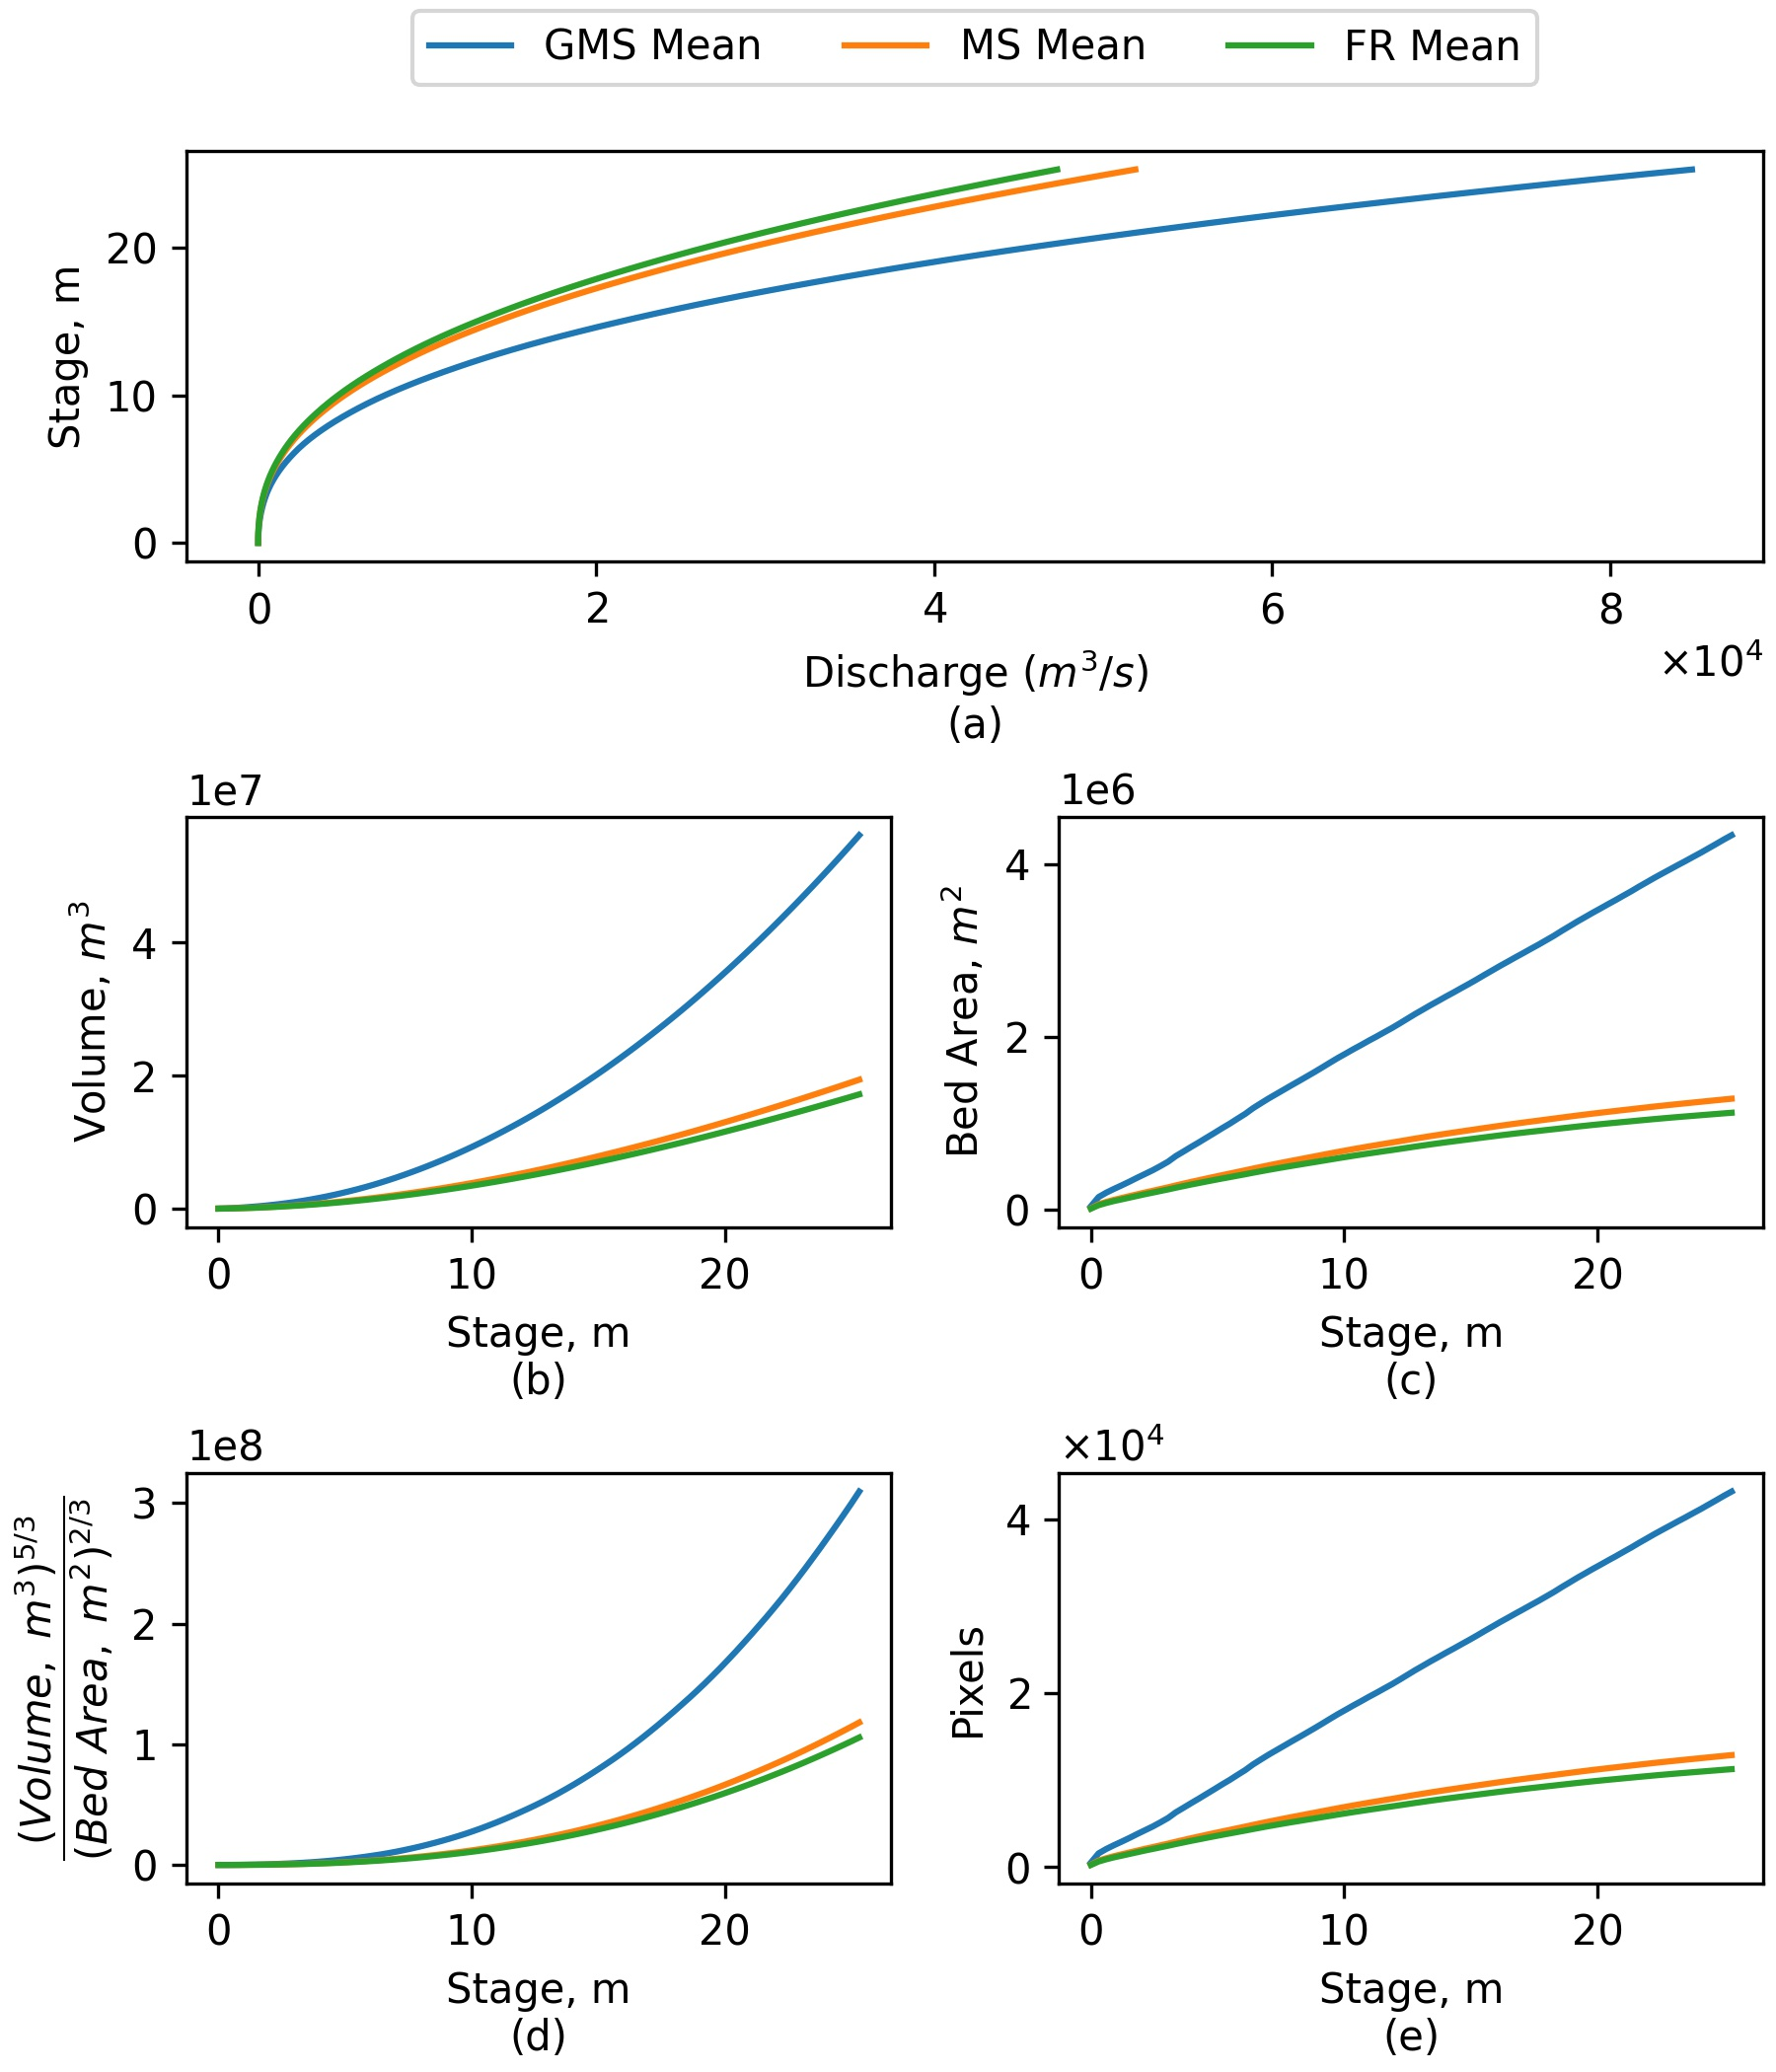
\includegraphics[scale=1.0]{figures/rating_curve_comparison.jpg}
\caption{Illustrates average quantities for the three methods, FR, MS, and GMS, for each stage value (m). 
The values are (a) Discharge $m^3s^{-1}$, (b) Volume $m^3$, (c) Bed Area $m^2$, (d) a function of Volume and Bed Area, and (e) number of pixels.
}
\label{fig:rating_curve_comparison}
\end{figure}
%
%
\DIFdelbegin %DIFDELCMD < \begin{figure}[h!]
%DIFDELCMD < %%%
\DIFdelendFL \DIFaddbeginFL \begin{figure}[H]
\DIFaddendFL \centering
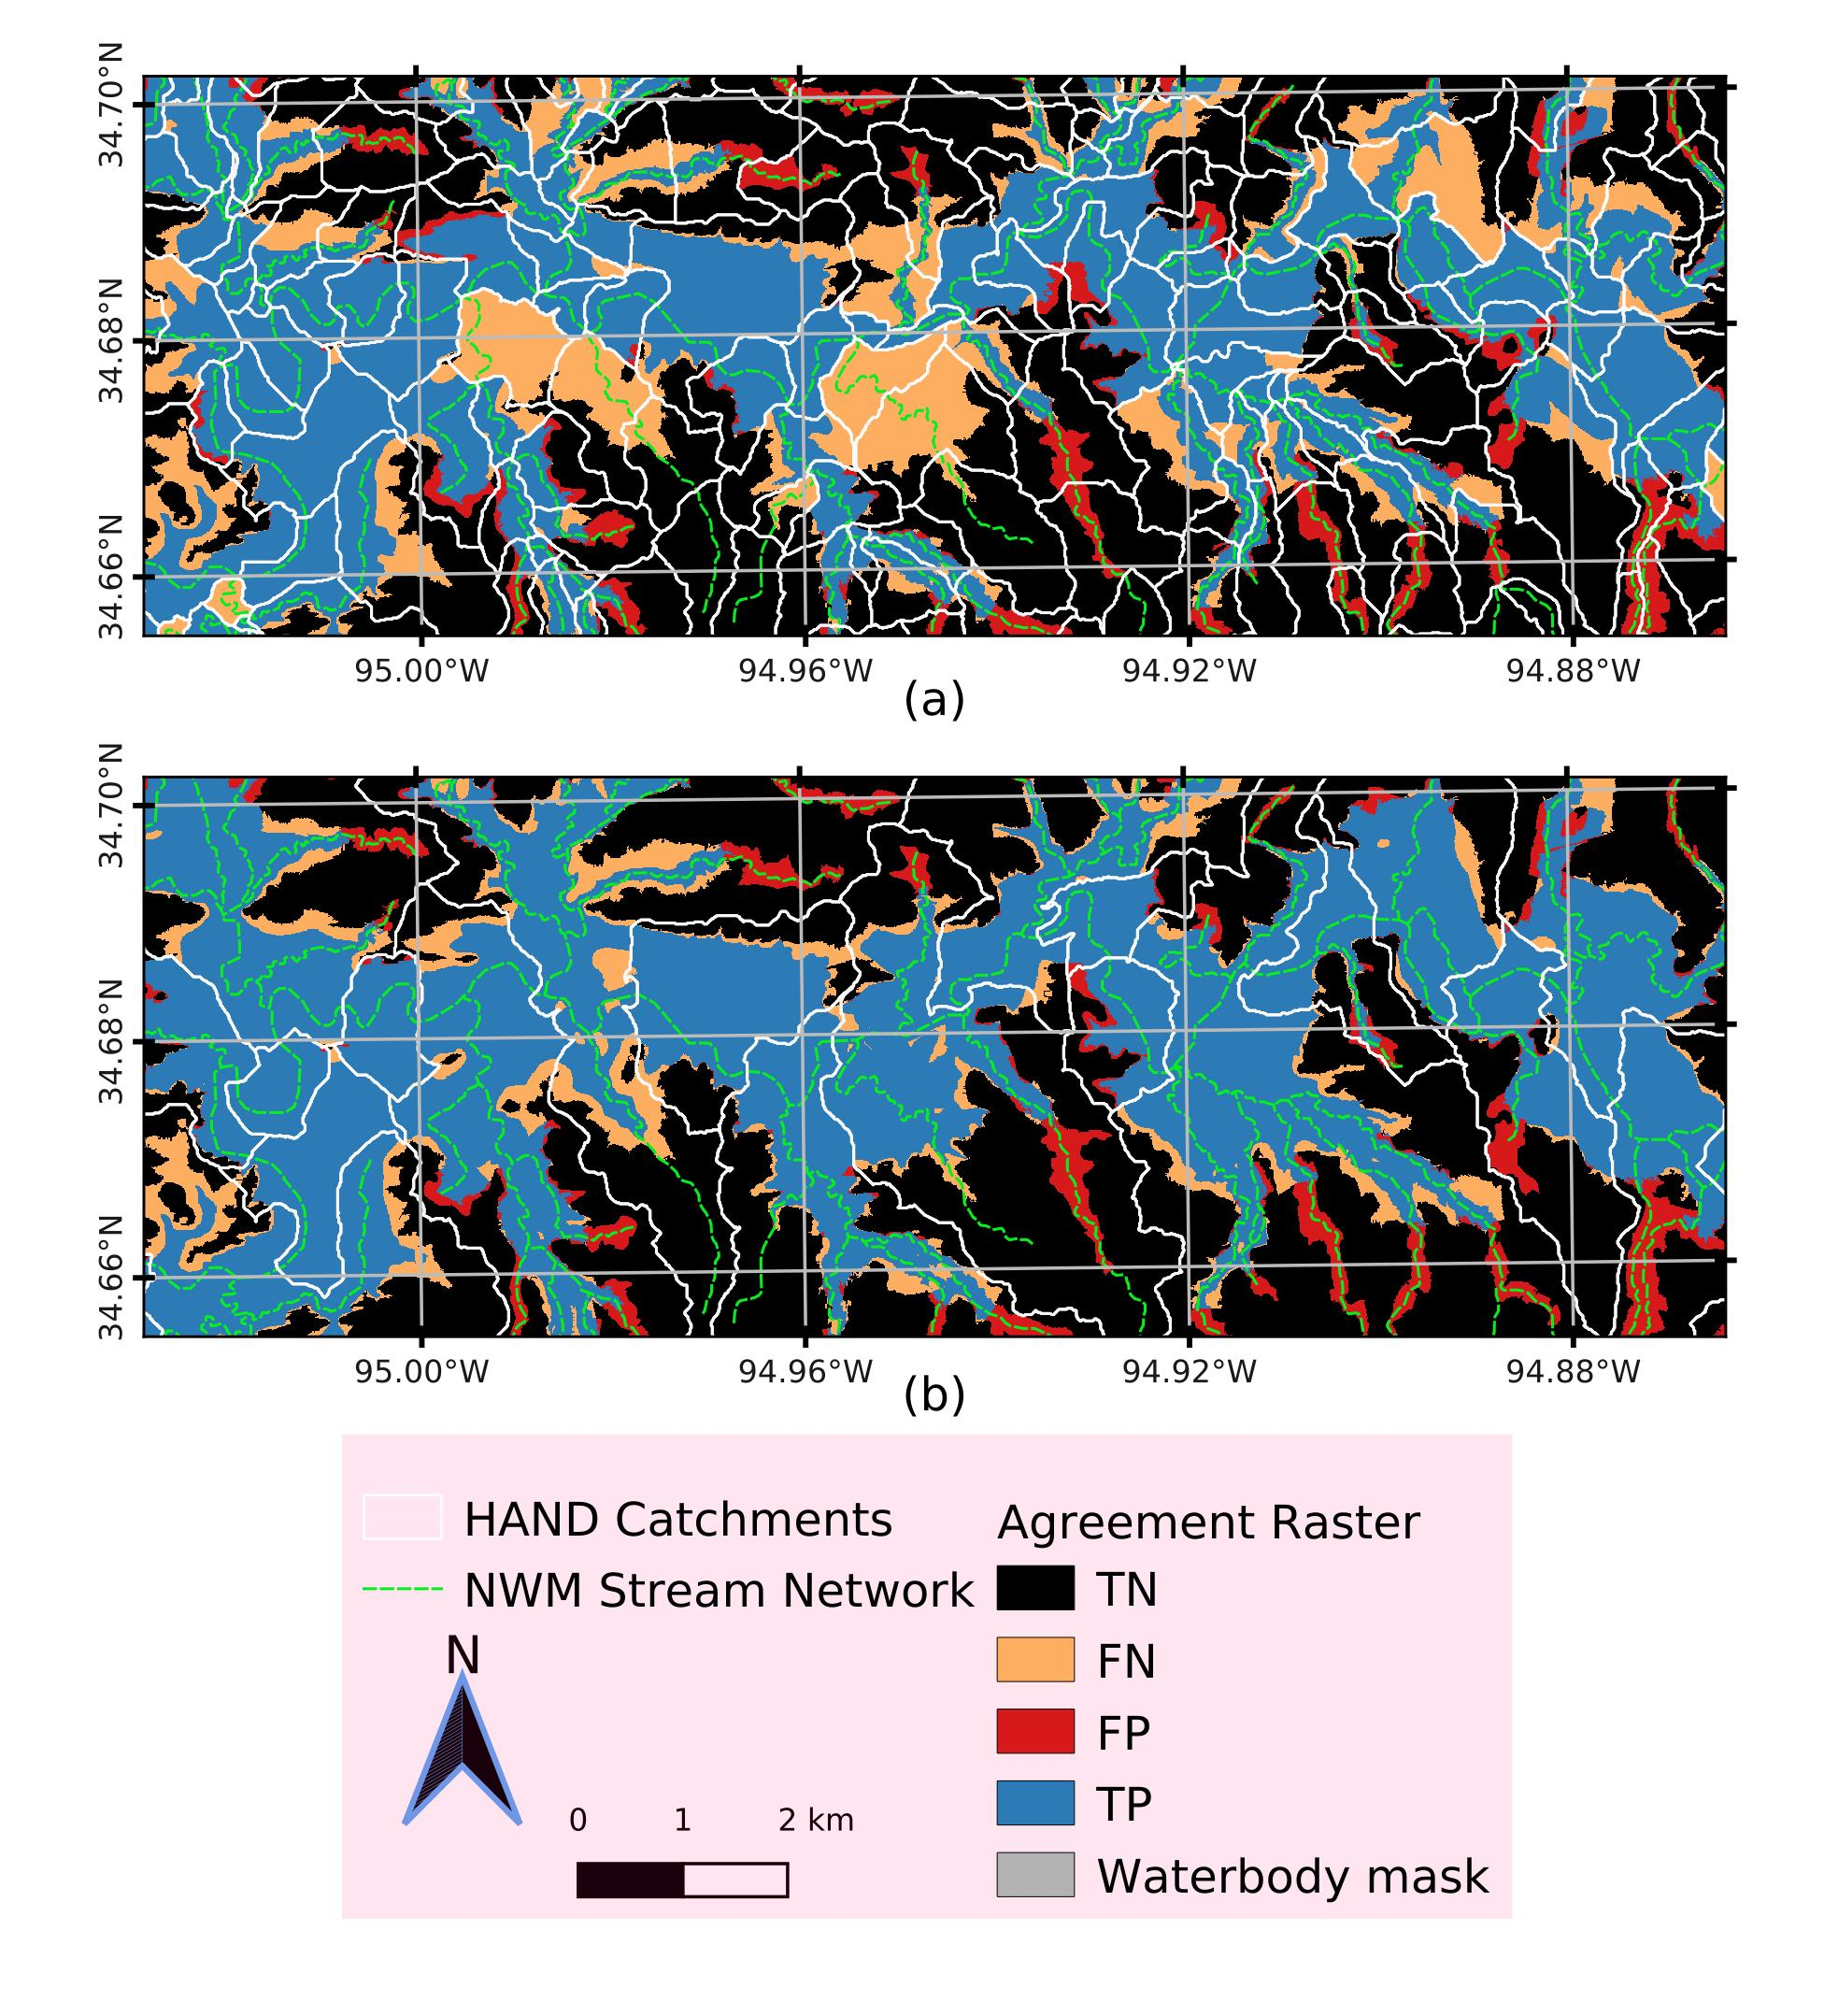
\includegraphics[scale=1.0]{figures/gms_enhancement.jpg}
\caption{OWP FIM inundation agreement, TP, FP, FN, and TN, with BLE HEC-RAS maps in HUC \DIFdelbeginFL \DIFdelFL{11140105.
}\DIFdelendFL \DIFaddbeginFL \DIFaddFL{11140105 at the 500 yr recurrence magnitude.
}\DIFaddendFL Catchment boundaries and stream lines are shown in white and dotted green, respectively.
Sub-figure (a) shows agreement of FR HAND denoting significant areas of under-prediction due to junctions and catchment boundaries.
Meanwhile, (b) shows the agreement for GMS and much larger catchments leading to much better inundation agreement for this given reach. 
Overall, this illustrates the benefits of stream order reduction for deriving HAND datasets.
}
\label{fig:gms_enhancement}
\end{figure}
%
 %
% Conclusions
\clearpage % this clears figures before references
%%%%%%%%%%%%%%%%%%%%%%%%%%%%%%%%%%%%%%%%%%%%%%%%%%%%%%%%
%%%%%%%%%%%%%%%%%%%%%%%%%%%%%%%%%%%%%%%%%%%%%%%%%%%%%%%%
\section{Conclusions}
\label{sec:conclusions}
%%%%%%%%%%%%%%%%%%%%%%%%%%%%%%%%%%%%%%%%%%%%%%%%%%%%%%%%
%%%%%%%%%%%%%%%%%%%%%%%%%%%%%%%%%%%%%%%%%%%%%%%%%%%%%%%%
%
Floods present a significant, under-served, and expanding risk to life, property, and resources.
Previous flood forecasting systems lacked the coverage to adequately inform society of these risks.
The National Water Model (NWM)\DIFaddbegin \DIFadd{, }\DIFaddend developed by the National Oceanic and Atmospheric Administration's \DIFaddbegin \DIFadd{(NOAA) }\DIFaddend Office of Water Prediction \DIFdelbegin \DIFdel{, along with partners, }\DIFdelend \DIFaddbegin \DIFadd{(OWP) and the National Center for Atmospheric Research (NCAR), }\DIFaddend provides increased spatial coverage and resolution as well as additional forecast time horizons on mostly hourly intervals.
Additional \DIFdelbegin \DIFdel{processing }\DIFdelend \DIFaddbegin \DIFadd{modeling }\DIFaddend is required to convert streamflows from the NWM to river stages and finally to flood inundation maps (FIM).
Height Above Nearest Drainage (HAND) is a means of detrending digital elevations maps (DEM) by normalizing elevation to the nearest relevant drainage point.
HAND coupled with the use of reach averaged synthetic rating curves (SRC) provide such a means of creating continental scale FIM capabilities at high resolutions (1/3 arc-second, 10 m) and high temporal frequencies (up to 1 hr).
Scalable, open-source software\DIFaddbegin \DIFadd{, known as OWP FIM, }\DIFaddend was developed to produce HAND and associated datasets (catchments, SRCs, and cross-walking data) for the NWM forecasting area including Hawaii and Puerto Rico \cite{inundationMapping2022}.
HAND is produced using the latest hydro-conditioning techniques to enforce monotonically decreasing elevations including stream burning, levee enforcement, pit-filling, stream channel excavation, thalweg breaching, headwater seeding, stream reach resampling, and more. 
Finally, we \DIFdelbegin \DIFdel{use }\DIFdelend \DIFaddbegin \DIFadd{used }\DIFaddend this implementation to investigate the skill of the FIMs by varying the scale of the processing units used to derive HAND.
\DIFaddbegin \DIFadd{FIM skill was evaluated over large spatial scales by comparison to HEC-RAS 1D models.
}

\DIFadd{The main contribution and conclusion of this work centers around a fundamental limitation in HAND based FIM which is a failure to account for multiple possible sources of fluvial inundation since HAND only considers inundation from the nearest drainage line.
}\DIFaddend We illustrate that reducing the Horton-Strahler stream order of a HAND processing unit down to one enhances skill by significantly reducing false negatives at junctions of major streams.
\DIFdelbegin \DIFdel{This }\DIFdelend \DIFaddbegin \DIFadd{In order to reduce stream order of the NWM stream network for HAND computation, we dissected the NWM network into two simpler units of singular Horton-Strahler stream order and mosaiced the resulting FIMs derived from each.
The NWM Mainstems (MS) stream network, which covers roughly 4-5\% of the NWM Full Resolution (FR) network, spans all established forecasting points in the Advanced Hydrologic Prediction System (AHPS) and downstream reaches.
The inundation from MS derived HAND is mosaiced together with the inundation of FR derived HAND.
Extending order reduction to the entire network, the Generalized Mainstem (GMS) technique discretizes the NWM FR network into level paths (LP) of unit stream order for HAND computation.
All LP based FIM derived from LP based HAND datasets are mosaiced together to form one seamless FIM.
Dissecting the stream network into regions of LPs with unit stream order is necessary because HAND has a ``nearest drainage'' limitation meaning it only accounts for riverine inundation sourced from the nearest drainage line.
In our evaluation of this technique, we observe that HAND based FIM improves in skill as we extend from nearest drainage inundation in FR to multiple drainage support in MS for only 4-5\% of the FR network.
Extending multiple drainage support to the entire FR network with GMS based HAND improves skill at around the same magnitude that MS improved upon FR.
Thus we conclude that deriving HAND with independent stream networks of unit Horton-Strahler stream order enhances the skill of FIM but offers diminishing returns as we extend from 4-5\% of the network with MS to 100\% of the network with GMS since deriving HAND and FIMs at these localized scale does add computational expense.
}

\DIFadd{This primary contribution }\DIFaddend also affects the parameters used to compute stage-discharge relationships \DIFdelbegin \DIFdel{biasing }\DIFdelend \DIFaddbegin \DIFadd{shifting }\DIFaddend discharge higher at given stages which reduced the rate of false positives.
\DIFdelbegin \DIFdel{FIM skill was evaluated over large spatial scales by comparsion to HEC-RAS 1D models.
Further investment in the SRC's is warranted by accounting for bathymetric errors inherited by the DEM and better accounting for localized friction values at varying flow magnitudes}\DIFdelend \DIFaddbegin \DIFadd{This shift in SRC behavior is driven by larger catchments that influence reach averaged geometric parameters in the Manning's equation.
Related to SRCs, we noted better results and more sensitivity to unit stream order networks with the higher Manning's n value of 0.12 when compared to 0.06 for high magnitude events at 1\% (100 year or yr) and 0.2\% (500 year or yr) recurrence intervals.
Additionally, we noted better performance for more intense 500 yr events which we attribute to a stronger influence of poor quality bathymetric data in 100 yr magnitude inundation extents.
While the AGREE DEM procedure is meant to add some bathymetry primarily motivated to enhance catchment and stream line delineation, it does introduce three parameters that have major implications in the quality of SRCs and the resulting FIMs}\DIFaddend .
Utilizing the highest resolution Lidar and bathymetric data should also improve the vertical accuracy of HAND and better account for fine grain features that greatly affect inundation extents.
\DIFaddbegin \DIFadd{We leave questions related to Manning's n localization as well as bathymetry integration, estimation, and/or calibration open for future research to answer.
Two other issues left open for improvement include the integration of higher resolution Lidar-based digital elevation maps (DEM) as well as the use of physics-based models for continental scale, high resolution forecasting applications.
}\DIFaddend Due to inherent limitations with HAND, scalable, physics-based methods are necessary to consider to provide a better representation of flood extent dynamics in steady and unsteady conditions.
 %
%DIF >  Open Research
\DIFaddbegin \clearpage
%DIF > %%%%%%%%%%%%%%%%%%%%%%%%%%%%%%%%%%%%%%%%%%%%%%%%%%%%%%%
%DIF > %%%%%%%%%%%%%%%%%%%%%%%%%%%%%%%%%%%%%%%%%%%%%%%%%%%%%%%
\section*{\DIFadd{Open Research}}
%DIF > \openresearch
%DIF > %%%%%%%%%%%%%%%%%%%%%%%%%%%%%%%%%%%%%%%%%%%%%%%%%%%%%%%
%DIF > %%%%%%%%%%%%%%%%%%%%%%%%%%%%%%%%%%%%%%%%%%%%%%%%%%%%%%%
\DIFaddend %
\DIFaddbegin \DIFadd{National Water Model (NWM) data used in this study includes the hydrofabric related datasets \mbox{%DIFAUXCMD
\cite{nwm2022hydrofabric} }\hskip0pt%DIFAUXCMD
including catchments, streamlines, and reservoirs \mbox{%DIFAUXCMD
\cite{nwm2022hydrofabric}}\hskip0pt%DIFAUXCMD
.
These are furnished by the National Oceanic and Atmospheric Administration (NOAA) Office of Water Prediction (OWP) via an Earth Science Information Partners (ESIP) Amazon Web Services (AWS) S3 Bucket \mbox{%DIFAUXCMD
\cite{esipData2022}}\hskip0pt%DIFAUXCMD
.
OWP Flood Inundation Mapping (FIM) capabilities rely extensively on the use of the National Hydrography Plus High Resolution (NHDPlusHR) datasets including BurnLineEvents \mbox{%DIFAUXCMD
\cite{nhdplus2022vectors}}\hskip0pt%DIFAUXCMD
, value-added attributes (VAA) \mbox{%DIFAUXCMD
\cite{nhdplus2022vectors}}\hskip0pt%DIFAUXCMD
, water boundaries (WBD) or hydrologic unit code (HUC) geometries \mbox{%DIFAUXCMD
\cite{nhdplus2022wbd}}\hskip0pt%DIFAUXCMD
, and digital elevation maps (DEM) \mbox{%DIFAUXCMD
\cite{nhdplus2022dems}}\hskip0pt%DIFAUXCMD
.
Some additional datasets for processing include the National Levee Database (NLD) furnished by the United States Army Core of Engineers (USACE) \mbox{%DIFAUXCMD
\cite{engineers2016national}}\hskip0pt%DIFAUXCMD
, Land-sea border from the Great Lakes Hydrography Dataset (GLHD) furnished by the Great Lakes Aquatic Habitat Framework (GLAHF) \mbox{%DIFAUXCMD
\cite{GreatLakesHydrographyDataset}}\hskip0pt%DIFAUXCMD
, and a Land-sea border provided by OpenStreetMap (OSM) \mbox{%DIFAUXCMD
\cite{osm2021landsea}}\hskip0pt%DIFAUXCMD
.
Evaluation data was furnished by Interagency Flood Risk Management (InFRM) consortium including cross-sections and flood depths \mbox{%DIFAUXCMD
\cite{fema2021base,fema2021estimated}}\hskip0pt%DIFAUXCMD
.
Additionally, some FIM hydrofabric data including HAND grids, catchments, streamlines, synthetic rating curves, and cross-walk tables are available on the ESIP bucket \mbox{%DIFAUXCMD
\cite{esipData2022}}\hskip0pt%DIFAUXCMD
.
}

\DIFadd{Software used in preprocessing data, producing FIM hydrofrabic, generating FIM, computing metrics, and conducting analysis is available from a publicly available Github repository called ``inundation-mapping'' from the ``NOAA-OWP'' organization \mbox{%DIFAUXCMD
\cite{inundationMapping2022}}\hskip0pt%DIFAUXCMD
.
 %DIF > 
%DIF >  Acknowledgments
}\clearpage %DIF >  this clears figures before references
%DIF > %%%%%%%%%%%%%%%%%%%%%%%%%%%%%%%%%%%%%%%%%%%%%%%%%%%%%%%
%DIF > %%%%%%%%%%%%%%%%%%%%%%%%%%%%%%%%%%%%%%%%%%%%%%%%%%%%%%%
%DIF >  Acknowledgments
\acknowledgments
%DIF > %%%%%%%%%%%%%%%%%%%%%%%%%%%%%%%%%%%%%%%%%%%%%%%%%%%%%%%
%DIF > %%%%%%%%%%%%%%%%%%%%%%%%%%%%%%%%%%%%%%%%%%%%%%%%%%%%%%%
%DIF > 
\DIFadd{This work was funded by the Office of Water Prediction (OWP) which is part of the National Oceanic and Atmospheric Administration's (NOAA) National Weather Service (NWS).
Lynker, under contract with OWP, facilitated this work and computational resources used in research and development.
We would like to thank some notable contributors of this work including Chief Scientist at OWP, Fred Ogden for his technical expertise.
Additionally, David Blodgett from the United States Geolgical Survey (USGS) Water Mission Area was instrumental in helping define level paths and other hydrographic work.
More information on code availability, usage, and data retrieval for OWP FIM is available on GitHub \mbox{%DIFAUXCMD
\cite{inundationMapping2022}}\hskip0pt%DIFAUXCMD
.
Thanks to the Earth and Space Science Informatics Partnership (ESIP) for storing data from this study for public use and dissemination helping to provide transparent datasets for further collaboration with the research community \mbox{%DIFAUXCMD
\cite{esipData2022}}\hskip0pt%DIFAUXCMD
.
 %DIF > 
%DIF >  Bibliography
}\clearpage %DIF >  this clears figures before references
\bibliography{bibliography/owp_fim4_2022}
%DIF > 
\DIFaddend %%

%  Numbered lines in equations:
%  To add line numbers to lines in equations,
%  \begin{linenomath*}
%  \begin{equation}
%  \end{equation}
%  \end{linenomath*}


%% Enter Figures and Tables near as possible to where they are first mentioned:
%
% DO NOT USE \psfrag or \subfigure commands.
%
% Figure captions go below the figure.
%\section{= enter section title =}
%Text here ===>>>
%\section{= enter section title =}
%Text here ===>>>
%%

%  Numbered lines in equations:
%  To add line numbers to lines in equations,
%  \begin{linenomath*}
%  \begin{equation}
%  \end{equation}
%  \end{linenomath*}



%% Enter Figures and Tables near as possible to where they are first mentioned:
%
% DO NOT USE \psfrag or \subfigure commands.
%
% Figure captions go below the figure.
% Table titles go above tables;  other caption information
%  should be placed in last line of the table, using
% \multicolumn2l{$^a$ This is a table note.}
%
%----------------
% EXAMPLE FIGURES
%
% \begin{figure}
% \includegraphics{example.png}
% \caption{caption}
% \end{figure}
%
% Giving latex a width will help it to scale the figure properly. A simple trick is to use \textwidth. Try this if large figures run off the side of the page.
% \begin{figure}
% \noindent\includegraphics[width=\textwidth]{anothersample.png}
%\caption{caption}
%\label{pngfiguresample}
%\end{figure}
%
%
% If you get an error about an unknown bounding box, try specifying the width and height of the figure with the natwidth and natheight options. This is common when trying to add a PDF figure without pdflatex.
% \begin{figure}
% \noindent\includegraphics[natwidth=800px,natheight=600px]{samplefigure.pdf}
%\caption{caption}
%\label{pdffiguresample}
%\end{figure}
%
%
% PDFLatex does not seem to be able to process EPS figures. You may want to try the epstopdf package.
%

%
% ---------------
% EXAMPLE TABLE
%
% \begin{table}
% \caption{Time of the Transition Between Phase 1 and Phase 2$^{a}$}
% \centering
% \begin{tabular}{l c}
% \hline
%  Run  & Time (min)  \\
% \hline
%   $l1$  & 260   \\
%   $l2$  & 300   \\
%   $l3$  & 340   \\
%   $h1$  & 270   \\
%   $h2$  & 250   \\
%   $h3$  & 380   \\
%   $r1$  & 370   \\
%   $r2$  & 390   \\
% \hline
% \multicolumn{2}{l}{$^{a}$Footnote text here.}
% \end{tabular}
% \end{table}

%% SIDEWAYS FIGURE and TABLE
% AGU prefers the use of {sidewaystable} over {landscapetable} as it causes fewer problems.
%
% \begin{sidewaysfigure}
% \includegraphics[width=20pc]{figsamp}
% \caption{caption here}
% \label{newfig}
% \end{sidewaysfigure}
%
%  \begin{sidewaystable}
%  \caption{Caption here}
% \label{tab:signif_gap_clos}
%  \begin{tabular}{ccc}
% one&two&three\\
% four&five&six
%  \end{tabular}
%  \end{sidewaystable}

%% If using numbered lines, please surround equations with \begin{linenomath*}...\end{linenomath*}
%\begin{linenomath*}
%\begin{equation}
%y|{f} \sim g(m, \sigma),
%\end{equation}
%\end{linenomath*}

%%% End of body of article

%%%%%%%%%%%%%%%%%%%%%%%%%%%%%%%%
%% Optional Appendix goes here
%
% The \appendix command resets counters and redefines section heads
%
% After typing \appendix
%
%\section{Here Is Appendix Title}
% will show
% A: Here Is Appendix Title
%
%\appendix
%\section{Here is a sample appendix}

%%%%%%%%%%%%%%%%%%%%%%%%%%%%%%%%%%%%%%%%%%%%%%%%%%%%%%%%%%%%%%%%
%
% Optional Glossary, Notation or Acronym section goes here:
%
%%%%%%%%%%%%%%
% Glossary is only allowed in Reviews of Geophysics
%  \begin{glossary}
%  \term{Term}
%   Term Definition here
%  \term{Term}
%   Term Definition here
%  \term{Term}
%   Term Definition here
%  \end{glossary}

%
%%%%%%%%%%%%%%
% Acronyms
%   \begin{acronyms}
%   \acro{Acronym}
%   Definition here
%   \acro{EMOS}
%   Ensemble model output statistics
%   \acro{ECMWF}
%   Centre for Medium-Range Weather Forecasts
%   \end{acronyms}

%
%%%%%%%%%%%%%%
% Notation
%   \begin{notation}
%   \notation{$a+b$} Notation Definition here
%   \notation{$e=mc^2$}
%   Equation in German-born physicist Albert Einstein's theory of special
%  relativity that showed that the increased relativistic mass ($m$) of a
%  body comes from the energy of motion of the body—that is, its kinetic
%  energy ($E$)—divided by the speed of light squared ($c^2$).
%   \end{notation}




%%%%%%%%%%%%%%%%%%%%%%%%%%%%%%%%%%%%%%%%%%%%%%%%%%%%%%%%%%%%%%%%
%
%  ACKNOWLEDGMENTS
%
% The acknowledgments must list:
%
% >>>>	A statement that indicates to the reader where the data
% 	supporting the conclusions can be obtained (for example, in the
% 	references, tables, supporting information, and other databases).
%
% 	All funding sources related to this work from all authors
%
% 	Any real or perceived financial conflicts of interests for any
%	author
%
% 	Other affiliations for any author that may be perceived as
% 	having a conflict of interest with respect to the results of this
% 	paper.
%
%
% It is also the appropriate place to thank colleagues and other contributors.
% AGU does not normally allow dedications.
\DIFdelbegin %DIFDELCMD < 

%DIFDELCMD < \acknowledgments
%DIFDELCMD < %%%
\DIFdel{This work was funded by the OWP which is part of NOAA's National Weather Service.
Lynker, under contract with OWP, facilitated this work and computational resources used in research and development.
We would like to thank some notable contributors of this work including Chief Scientist at OWP, Fred Ogden for his technical expertise.
Additionally, David Blodgett from the USGS Water Mission Area was instrumental in helping define level paths and other hydrographic work.
More information on code availability, usage, and data retrieval for OWP FIM is available on GitHub \mbox{%DIFAUXCMD
\cite{inundationMapping2022}}\hskip0pt%DIFAUXCMD
.
Thanks to the Earth and Space Science Informatics Partnership (ESIP) for storing data from this study for public use and dissemination helping to provide transparent datasets for further collaboration with the research community \mbox{%DIFAUXCMD
\cite{esipData2022}}\hskip0pt%DIFAUXCMD
.
%DIF < The [type of data] data used for [brief context, description] in the study are available at [repository, source name] via [DOI, persistent identifier link] with  [license, access conditions] [optional in-text citation in References]
%DIF < [Version number] of the [software name] used for [brief context, description of what the software was used for] is preserved at [DOI, persistent identifier link], available via [license type, access conditions] and developed openly at [software development platform link].* [optional in-text citation in References].
}%DIFDELCMD < 

%DIFDELCMD < %%%
\DIFdelend %% ------------------------------------------------------------------------ %%
%% References and Citations

%%%%%%%%%%%%%%%%%%%%%%%%%%%%%%%%%%%%%%%%%%%%%%%
%
% \bibliography{<name of your .bib file>} don't specify the file extension
%
% don't specify bibliography style
%%%%%%%%%%%%%%%%%%%%%%%%%%%%%%%%%%%%%%%%%%%%%%%
%
\DIFdelbegin %DIFDELCMD < \clearpage %%%
%DIF <  this clears figures before references
%DIFDELCMD < \bibliography{bibliography/owp_fim4_2022}
%DIFDELCMD < %%%
\DIFdelend %
%Reference citation instructions and examples:
%
% Please use ONLY \cite and \citeA for reference citations.
% \cite for parenthetical references
% ...as shown in recent studies (Simpson et al., 2019)
% \citeA for in-text citations
% ...Simpson et al. (2019) have shown...
%
%
%...as shown by \citeA{jskilby}.
%...as shown by \citeA{lewin76}, \citeA{carson86}, \citeA{bartoldy02}, and \citeA{rinaldi03}.
%...has been shown \cite{jskilbye}.
%...has been shown \cite{lewin76,carson86,bartoldy02,rinaldi03}.
%... \cite <i.e.>[]{lewin76,carson86,bartoldy02,rinaldi03}.
%...has been shown by \cite <e.g.,>[and others]{lewin76}.
%
% apacite uses < > for prenotes and [ ] for postnotes
% DO NOT use other cite commands (e.g., \citet, \citep, \citeyear, \nocite, \citealp, etc.).
%



\end{document}



%%%% More Information and Advice:

%% ------------------------------------------------------------------------ %%
%
%  SECTION HEADS
%
%% ------------------------------------------------------------------------ %%

% Capitalize the first letter of each word (except for
% prepositions, conjunctions, and articles that are
% three or fewer letters).

% AGU follows standard outline style; therefore, there cannot be a section 1 without
% a section 2, or a section 2.3.1 without a section 2.3.2.
% Please make sure your section numbers are balanced.
% ---------------
% Level 1 head
%
% Use the \section{} command to identify level 1 heads;
% type the appropriate head wording between the curly
% brackets, as shown below.
%
%An example:
%\section{Level 1 Head: Introduction}
%
% ---------------
% Level 2 head
%
% Use the \subsection{} command to identify level 2 heads.
%An example:
%\subsection{Level 2 Head}
%
% ---------------
% Level 3 head
%
% Use the \subsubsection{} command to identify level 3 heads
%An example:
%\subsubsection{Level 3 Head}
%
%---------------
% Level 4 head
%
% Use the \subsubsubsection{} command to identify level 3 heads
% An example:
%\subsubsubsection{Level 4 Head} An example.
%
%% ------------------------------------------------------------------------ %%
%
%  IN-TEXT LISTS
%
%% ------------------------------------------------------------------------ %%
%
% Do not use bulleted lists; enumerated lists are okay.
% \begin{enumerate}
% \item
% \item
% \item
% \end{enumerate}
%
%% ------------------------------------------------------------------------ %%
%
%  EQUATIONS
%
%% ------------------------------------------------------------------------ %%

% Single-line equations are centered.
% Equation arrays will appear left-aligned.

Math coded inside display math mode \[ ...\]
 will not be numbered, e.g.,:
 \[ x^2=y^2 + z^2\]

 Math coded inside \begin{equation} and \end{equation} will
 be automatically numbered, e.g.,:
 \begin{equation}
 x^2=y^2 + z^2
 \end{equation}


% To create multiline equations, use the
% \begin{eqnarray} and \end{eqnarray} environment
% as demonstrated below.
\begin{eqnarray}
  x_{1} & = & (x - x_{0}) \cos \Theta \nonumber \\
        && + (y - y_{0}) \sin \Theta  \nonumber \\
  y_{1} & = & -(x - x_{0}) \sin \Theta \nonumber \\
        && + (y - y_{0}) \cos \Theta.
\end{eqnarray}

%If you don't want an equation number, use the star form:
%\begin{eqnarray*}...\end{eqnarray*}

% Break each line at a sign of operation
% (+, -, etc.) if possible, with the sign of operation
% on the new line.

% Indent second and subsequent lines to align with
% the first character following the equal sign on the
% first line.

% Use an \hspace{} command to insert horizontal space
% into your equation if necessary. Place an appropriate
% unit of measure between the curly braces, e.g.
% \hspace{1in}; you may have to experiment to achieve
% the correct amount of space.


%% ------------------------------------------------------------------------ %%
%
%  EQUATION NUMBERING: COUNTER
%
%% ------------------------------------------------------------------------ %%

% You may change equation numbering by resetting
% the equation counter or by explicitly numbering
% an equation.

% To explicitly number an equation, type \eqnum{}
% (with the desired number between the brackets)
% after the \begin{equation} or \begin{eqnarray}
% command.  The \eqnum{} command will affect only
% the equation it appears with; LaTeX will number
% any equations appearing later in the manuscript
% according to the equation counter.
%

% If you have a multiline equation that needs only
% one equation number, use a \nonumber command in
% front of the double backslashes (\\) as shown in
% the multiline equation above.

% If you are using line numbers, remember to surround
% equations with \begin{linenomath*}...\end{linenomath*}

%  To add line numbers to lines in equations:
%  \begin{linenomath*}
%  \begin{equation}
%  \end{equation}
%  \end{linenomath*}



